% Options for packages loaded elsewhere
\PassOptionsToPackage{unicode}{hyperref}
\PassOptionsToPackage{hyphens}{url}
%
\documentclass[
  12pt,
]{article}
\usepackage{amsmath,amssymb}
\usepackage{lmodern}
\usepackage{iftex}
\ifPDFTeX
  \usepackage[T1]{fontenc}
  \usepackage[utf8]{inputenc}
  \usepackage{textcomp} % provide euro and other symbols
\else % if luatex or xetex
  \usepackage{unicode-math}
  \defaultfontfeatures{Scale=MatchLowercase}
  \defaultfontfeatures[\rmfamily]{Ligatures=TeX,Scale=1}
\fi
% Use upquote if available, for straight quotes in verbatim environments
\IfFileExists{upquote.sty}{\usepackage{upquote}}{}
\IfFileExists{microtype.sty}{% use microtype if available
  \usepackage[]{microtype}
  \UseMicrotypeSet[protrusion]{basicmath} % disable protrusion for tt fonts
}{}
\makeatletter
\@ifundefined{KOMAClassName}{% if non-KOMA class
  \IfFileExists{parskip.sty}{%
    \usepackage{parskip}
  }{% else
    \setlength{\parindent}{0pt}
    \setlength{\parskip}{6pt plus 2pt minus 1pt}}
}{% if KOMA class
  \KOMAoptions{parskip=half}}
\makeatother
\usepackage{xcolor}
\IfFileExists{xurl.sty}{\usepackage{xurl}}{} % add URL line breaks if available
\IfFileExists{bookmark.sty}{\usepackage{bookmark}}{\usepackage{hyperref}}
\hypersetup{
  pdftitle={Factors affecting inferences on natural mortality and associated environmental effects},
  pdfauthor={Timothy J. Miller1; Andrew Applegate; Greg Britten; Elizabeth N. Brooks; Gavin Fay; Alex Hansell; Christopher M. Legault; Brandon Muffley; Brian C. Stock; John Wiedenmann},
  hidelinks,
  pdfcreator={LaTeX via pandoc}}
\urlstyle{same} % disable monospaced font for URLs
\usepackage[margin=1in]{geometry}
\usepackage{graphicx}
\makeatletter
\def\maxwidth{\ifdim\Gin@nat@width>\linewidth\linewidth\else\Gin@nat@width\fi}
\def\maxheight{\ifdim\Gin@nat@height>\textheight\textheight\else\Gin@nat@height\fi}
\makeatother
% Scale images if necessary, so that they will not overflow the page
% margins by default, and it is still possible to overwrite the defaults
% using explicit options in \includegraphics[width, height, ...]{}
\setkeys{Gin}{width=\maxwidth,height=\maxheight,keepaspectratio}
% Set default figure placement to htbp
\makeatletter
\def\fps@figure{htbp}
\makeatother
\setlength{\emergencystretch}{3em} % prevent overfull lines
\providecommand{\tightlist}{%
  \setlength{\itemsep}{0pt}\setlength{\parskip}{0pt}}
\setcounter{secnumdepth}{5}
\newlength{\cslhangindent}
\setlength{\cslhangindent}{1.5em}
\newlength{\csllabelwidth}
\setlength{\csllabelwidth}{3em}
\newlength{\cslentryspacingunit} % times entry-spacing
\setlength{\cslentryspacingunit}{\parskip}
\newenvironment{CSLReferences}[2] % #1 hanging-ident, #2 entry spacing
 {% don't indent paragraphs
  \setlength{\parindent}{0pt}
  % turn on hanging indent if param 1 is 1
  \ifodd #1
  \let\oldpar\par
  \def\par{\hangindent=\cslhangindent\oldpar}
  \fi
  % set entry spacing
  \setlength{\parskip}{#2\cslentryspacingunit}
 }%
 {}
\usepackage{calc}
\newcommand{\CSLBlock}[1]{#1\hfill\break}
\newcommand{\CSLLeftMargin}[1]{\parbox[t]{\csllabelwidth}{#1}}
\newcommand{\CSLRightInline}[1]{\parbox[t]{\linewidth - \csllabelwidth}{#1}\break}
\newcommand{\CSLIndent}[1]{\hspace{\cslhangindent}#1}
\usepackage{url}
\usepackage{setspace}
%\singlespacing
%\onehalfspacing
%\doublespacing
\usepackage{lineno}
%\linenumbers
\usepackage[belowskip=0pt,aboveskip=0pt]{caption}
\usepackage{relsize}
\newcommand{\Fmsy}{\ensuremath{F_{\text{MSY}}}\xspace}
\newcommand{\Fspr}[1]{\ensuremath{F_{\text{{#1}\%}}}\xspace}
\newcommand{\afrb}{Alaska Fishery Research Bulletin\xspace}
\newcommand{\ajms}{African Journal of Marine Science\xspace}
\newcommand{\amb}{Advances in Marine Biology\xspace}
\newcommand{\bms}{Bulletin of Marine Science\xspace}
\newcommand{\bjssf}{Bulletin of the Japanese Society of Scientific Fisheries\xspace}
\newcommand{\cb}{Conservation Biology\xspace}
\newcommand{\cjfas}{Canadian Journal of Fisheries and Aquatic Sciences\xspace}
\newcommand{\ea}{Ecological Applications\xspace}
\newcommand{\eer}{Evolutionary Ecology Research\xspace}
\newcommand{\elet}{Ecology Letters\xspace}
\newcommand{\emod}{Ecological Modelling\xspace}
\newcommand{\ebf}{Environmental Biology of Fishes\xspace}
\newcommand{\ff}{Fish and Fisheries\xspace}
\newcommand{\fo}{Fisheries Oceanography\xspace}
\newcommand{\fr}{Fisheries Research\xspace}
\newcommand{\fb}{Fishery Bulletin\xspace}
\newcommand{\ijms}{ICES Journal of Marine Science\xspace}
\newcommand{\iccat}{Collective Volume of Scientific Papers ICCAT\xspace}
\newcommand{\jae}{Journal of Animal Ecology\xspace}
\newcommand{\jai}{Journal of Applied Ichthyology\xspace}
\newcommand{\jdc}{Journal Du Conseil International Pour L'exploration De La Mer\xspace}
\newcommand{\jdcp}{Journal Du Conseil Permanent International Pour L'exploration De La Mer\xspace}
\newcommand{\jembe}{Journal of Experimental Marine Biology and Ecology\xspace}
\newcommand{\jfb}{Journal of Fish Biology\xspace}
\newcommand{\jsr}{Journal of Sea Research\xspace}
\newcommand{\jtb}{Journal of Theoretical Biology\xspace}
\newcommand{\jfrbc}{Journal of the Fisheries Research Board of Canada\xspace}
\newcommand{\jnwafs}{Journal of Northwest Atlantic Fisheries Science\xspace}
\newcommand{\mcf}{Marine and Coastal Fisheries: Dynamics, Management, and Ecosystem Science\xspace}
\newcommand{\mb}{Marine Biology\xspace}
\newcommand{\meps}{Marine Ecology Progress Series\xspace}
\newcommand{\mfr}{Marine Fisheries Review\xspace}
\newcommand{\mpb}{Marine Pollution Bulletin\xspace}
\newcommand{\najfm}{North American Journal of Fisheries Management\xspace}
\newcommand{\nzjmfr}{New Zealand Journal of Marine and Freshwater Research\xspace}
\newcommand{\pnas}{Proceedings of the National Academy of Sciences USA\xspace}
\newcommand{\rpvrciemm}{Rapports et Proc\`es-Verbaux des R\'eunions. Conseil Internationale pour l'Exploration de la Mer\xspace}
\newcommand{\rpvrcpiemm}{Rapports et Proc\`es-Verbaux des R\'eunions. Conseil Permanent Internationale pour l'Exploration de la Mer\xspace}
\newcommand{\rfbf}{Reviews in Fish Biology and Fisheries\xspace}
\newcommand{\sajms}{South African Journal of Marine Science\xspace}
\newcommand{\tafs}{Transactions of the American Fisheries Society\xspace}

\newcommand{\anzjs}{Australian \& New Zealand Journal of Statistics\xspace}
\newcommand{\as}{Applied Statistics\xspace}
\newcommand{\csda}{Computational Statistics \& Data Analysis\xspace}
\newcommand{\ees}{Environmental and Ecological Statistics\xspace}
\newcommand{\jas}{Journal of Applied Statistics\xspace}
\newcommand{\jabes}{Journal of Agricultural, Biological, and Environmental Statistics\xspace}
\newcommand{\jasa}{Journal of the American Statistical Association\xspace}
\newcommand{\jrssb}{Journal of the Royal Statistical Society. Series B\xspace}
\newcommand{\sm}{Statistics in Medicine}

\usepackage{xspace}
\usepackage{bm}
\usepackage{caption,graphics}
\usepackage{graphicx}
\usepackage{makecell}
\renewcommand\figurename{Fig.}
\captionsetup{labelsep=period, singlelinecheck=false}
\newcommand{\changesize}[1]{\fontsize{#1pt}{#1pt}\selectfont}
\renewcommand{\arraystretch}{1.5}
\renewcommand\theadfont{}
\usepackage{booktabs}
\usepackage{longtable}
\usepackage{array}
\usepackage{multirow}
\usepackage{wrapfig}
\usepackage{float}
\usepackage{colortbl}
\usepackage{pdflscape}
\usepackage{tabu}
\usepackage{threeparttable}
\usepackage{threeparttablex}
\usepackage[normalem]{ulem}
\usepackage{makecell}
\usepackage{xcolor}
\ifLuaTeX
  \usepackage{selnolig}  % disable illegal ligatures
\fi
\usepackage[]{natbib}
\bibliographystyle{cjfas2.bst}

\title{Factors affecting inferences on natural mortality and associated
environmental effects}
\author{Timothy J. Miller\textsuperscript{1} \and Andrew
Applegate \and Greg Britten \and Elizabeth N. Brooks \and Gavin
Fay \and Alex Hansell \and Christopher M. Legault \and Brandon
Muffley \and Brian C. Stock \and John Wiedenmann}
\date{}

\begin{document}
\maketitle

\(^1\)corresponding author:
\href{mailto:timothy.j.miller@noaa.gov}{\nolinkurl{timothy.j.miller@noaa.gov}},
Northeast Fisheries Science Center, Woods Hole Laboratory, 166 Water
Street, Woods Hole, MA 02543 USA\\

\pagebreak

\hypertarget{summaryabstract}{%
\subsection*{Summary/Abstract}\label{summaryabstract}}
\addcontentsline{toc}{subsection}{Summary/Abstract}

We completed a large scale simulation study with 288 operating models
with 12 estimated models fit to each. The factors defining operating
model configuration inlcuded the source of process error on the
population (recruitment, recruitment and survival, recruitment and
natural mortality), the degree of temporal variation and autocorrelation
of the environmental covariate, the uncertainty in the observation of
the covariate, the uncertainty in indices and age composition
observations, fishing history, and the magnitude of the effect of the
covariate on natural mortality.

We found convergence of all estimation models was generally best when
operating models assumed process errors in recruitment and survival,
constant fishing rate, greater contrast in the true environmental
covariate, and lower uncertainty in corresponding observations. Reliable
convergence of all estimating models also occurred with the same process
errors in the operating model and a step-change in fishing, but this
also required lower uncertainty in index and age composition
observations. Estimating models with process errors on recruitment and
survival were unlikely to converge when the process errors in the
operating model did not match whereas estimating models with process
errors in recruitment and natural mortality converged for operating
models without this match in certain cases. Probability of convergence
generally decreased when the mean natural mortality rate parameter was
estimated.

AIC paragraph

Bias paragraph

These results suggest that models with covariate effects on M will be
most reliable when R+S is true, large contrast in the Recommendations
\#\#\# Keywords \{-\}

\pagebreak

\hypertarget{introduction}{%
\section*{Introduction}\label{introduction}}
\addcontentsline{toc}{section}{Introduction}

Here we conduct a simulation study with operating models varying by
degree of observation error uncertainty, sources of process error (M or
survival), fishing history, temporal variation in environmental
covariates, and magnitude of the effect of the covariate on natural
mortality. The simulations from these operating models are fitted with
estimating models that make alternative assumptions for sources of
process error, and whether (mean) M is estimated. We evaluate effects of
these factors on convergence of fitted models, whether AIC can correctly
determine the correct source of process error and correct assumption
about covariate effects on natural mortality, and the degree of bias in
relevant parameters and outputs of the assessment model.

\hypertarget{methods}{%
\section*{Methods}\label{methods}}
\addcontentsline{toc}{section}{Methods}

We used the WHAM package
\citep[][version 1.0.7, commit 77bbd94]{millerstock20,stockmiller21} to
configure all operating models and estimation models. This packages has
also been used to configure operating and estimating models for closed
loop simulations evaluating index-based assessment methods
\citep{legaultetal23} and is used for management of GB haddock,
butterfish, plaice, bluefish, and Atlantic cod stocks in the Northeast
US.

We completed a simulation study with a number of operating models. Many
of the characteristics of the operating models are the same as those
used by \citet{milleretal_project0_wp}. The factors defining the
configuration of each operating model which are described in detail in
subsequent sections include

\begin{itemize}
\item two configurations of fishing histories, 
\item two configurations of index and age composition observation error, 
\item four configurations of latent environmental covariate process errors, 
\item two configurations of environmental covariate observation uncertainty, 
\item three levels of covariate effects on natural mortality, and 
\item three configurations of sources of process errors for temporal changes in abundances at age. 
\end{itemize}

The full factorial of the levels of each factor results in 288 different
operating models. We simulated 100 data sets for each operating model
that included simulations of process errors.

For each simulated data set we fit a set of 12 estimating models. The
factors defining the configuration or each estimating model which are
also described in detail below include

\begin{itemize}
\item three configurations of sources of process errors for temporal changes in abundances at age, 
\item whether the (mean) natural mortality rate was estimated or assumed known at the true value, and
\item whether the effect of the environmental covariate on natural mortality was estimated.
\end{itemize}

We did not use the bias-correction feature for process errors or
observations described by \citet{stockmiller21} for operating and
estimating models. Simulations were all carried out on the University of
Massachusetts Green High-Performance Computing Cluster. Code for
completing the simulations and summarization of results can be found at
github.com/timjmiller/SSRTWG/ecov\_study/mortality.

\hypertarget{operating-models}{%
\subsection*{Operating models}\label{operating-models}}
\addcontentsline{toc}{subsection}{Operating models}

\hypertarget{population}{%
\subsubsection*{Population}\label{population}}
\addcontentsline{toc}{subsubsection}{Population}

The population model tracks 10 age classes: ages 1 to 10+ and we assume
spawning occurs 1/4 of the way through the year. The maturity at age was
a logistic curve with a50 = 2.89 and slope = 0.88 and assumed known in
all estimation models (Figure \ref{om_maturity}).

Weight at age was generated with a LVB growth function \[
L_a = L_{\infty}\left(1 - e^{-k(a - t_0)}\right)
\] where \(t_0 = 0\), \(L_\infty = 85\), and \(k = 0.3\), and a L-W
relationship such that \[
W_a = \theta_1 L_a^{\theta_2}
\] where \(\theta_1 = e^{-12.1}\) and \(\theta_2 = 3.2\) (Figure
\ref{om_waa}).

We assumed a Beverton-Holt stock recruit function with constant
pre-recruit mortality parameters (i.e., \(\alpha\) and \(\beta\)) for
all operating models. All post-recruit productivity components are
constant in the NAA and survey selectivity process error operating
models. Therefore steepness and unfished recruitment are also constant
over the time period for those operating models \citep{millerbrooks21}.
We specified unfished recruitment = \(R_0 = e^{10}\) and
\(\Fmsy = \Fspr[40] = 0.348\) equated to a steepness of 0.69 and
\(\alpha=0.60\) and \(\beta = 2.4 \times 10^{-5}\) for the \[
N_{1,y} = \frac{\alpha \text{SSB}_{y-1}}{1 + \beta \text{SSB}_{y-1}} 
\] Beverton-Holt parameterization (Figure \ref{om_sr}). For OMs without
process errors on natural mortality we assumed the rate was assumed 0.2.
For OMs with process errors on natural mortality the mean rate was 0.2.

Two alternative fishing histories were used for operating models. In the
first scenario, the stock experiences overfishing for the first 20 years
and fishing at \Fmsy for the last 20 years. In the second scenario, the
stock is fished at \Fmsy for the entire time period. The magnitude of
the overfishing assumptions is based on average estimates of overfishing
for NE groundfish stocks from \citet{wiedenmannetal19}.
\Citet{legaultetal23} also used similar approaches to defining fishing
mortality histories for operating models.

Initial population was configured at the equilibrium distribution
fishing at either \(F = 2.5\times \Fmsy\) or \(F = \Fmsy\) for the two
alternative fishing histories. That is for a deterministic model, the
age composition would not change over time when the fishing mortality
was constant at the respective level.

For operating models with time-varying random effects or covariate
effects on M, steepness is not constant, but we used the same alpha and
beta parameters as other operating models this equates to a steepness
and \(R_0\) at the mean of the time series process for M. For operating
models with time-varying random effects for fishery selectivity,
\Fmsy is also not constant however we use the same F history as other
operating models which corresponds to \Fmsy at the mean selectivity
parameters.

\hypertarget{environmental-covariate}{%
\subsubsection*{Environmental covariate}\label{environmental-covariate}}
\addcontentsline{toc}{subsubsection}{Environmental covariate}

In the WHAM model, environmental covariates are assumed to be described
as state-space processes with annual observations of the true latent
covariate. The latent covariate is assumed to be Gaussian AR1 \[
E_y|E_{y-1} \sim \text{N}\left(\mu_\text{Ecov}\left(1-\rho_\text{Ecov}\right) + \rho_\text{Ecov} E_{y-1}, \left(1-\rho_\text{Ecov}^2\right)\sigma^2_\text{Ecov}\right)
\] with marginal mean \(\mu_\text{Ecov}=0\) and variance
\(\sigma^2_\text{Ecov}\). The configuration of the latent environmental
covariate in the operating models have one of two alternate assumptions
about the marginal standard deviation and autocorrelation parameter:

\begin{itemize}
\item marginal standard deviation $\sigma_\text{Ecov} \in \{0.1, 0.5\}$
\item AR1 correlation $\rho_\text{Ecov} \in \{0, 0.5\}$
\end{itemize}

The observations of the latent environmental covariate are assumed to be
unbiased and Gaussian \[
\text{ecov}_y|E_y \sim \text{N}\left(E_y,\sigma^2_\text{ecov}\right)
\] The standard deviation of the environmental observations in the
operating models is one of two values:

\begin{itemize}
\item standard deviation $\in \{0.1, 0.5\}$
\end{itemize}

Figure \ref{om_ecov_example} provides example simulations of the latent
process and observations under the alternative configurations.

\hypertarget{random-effects-on-recruitment-survival-and-natural-mortality}{%
\subsubsection*{Random effects on recruitment, survival, and natural
mortality}\label{random-effects-on-recruitment-survival-and-natural-mortality}}
\addcontentsline{toc}{subsubsection}{Random effects on recruitment,
survival, and natural mortality}

Internally, WHAM treats natural mortality as a log-transformed parameter
\[
\log M_y = \beta_M + \beta_{\text{Ecov}} E_y + \varepsilon_{M,y}
\] that is a linear combination of a mean \(\beta_M\) and any annual
covariate \(\beta_{\text{Ecov}}\) and random effects marginally
distributed as \(\epsilon_{M,y} \sim \text{N}\left(0,\sigma_M^2\right)\)
\citep{stockmiller21}. For operating models with natural mortality
random effects, we assume the same standard deviation
\(\sigma_M = 0.3\).

The covariate effect is one of 3 alternative values in the operating
models:

\begin{itemize}
\item $\beta_\text{Ecov} \in \{0,0.25,0.5\}$
\end{itemize}

The parameters defining the simulated covariate time series, size of the
covariate effect, and any natural mortality random effects result in a
range of different levels of variation in annual natural mortality rates
(Figure \ref{M_example}).

As described by \citet{stockmiller21}, the model for process errors on
abundance at age in WHAM is \begin{equation}
  \text{log}N_{a,y}=\left\{
    \begin{array}{@{}lll@{}}
      \text{log} \left( f(SSB_{y-1}) \right) + \varepsilon_{1,y}, & \text{if}\ a = 1 \\
      \text{log} \left( N_{a-1,y-1} \right) - Z_{a-1,y-1} + \varepsilon_{a,y}, & \text{if}\ 1 < a < A \\
      \text{log} \left( N_{A-1,y-1} e^{-Z_{A-1,y-1}} + N_{A,y-1} e^{-Z_{A,y-1}} \right) + \varepsilon_{A,y}, & \text{if}\ a = A
    \end{array}\right.
\end{equation} We assume the the standard deviation of recruitment
deviations is
\(\text{SD}\left(\varepsilon_{1,y}\right) = \sigma_R = 0.5\) for all
operating models. For operating models with survival devations for older
ages, we assume the same standard deviations for all older ages
\(\text{SD}\left(\varepsilon_{a,y}\right) = \sigma_{2+} = 0.3\).

The alternative configurations of random effects on recruitment,
survival, and natural mortality are

\begin{itemize}
\item uncorrelated random effects on recruitment only ($\sigma_R = 0.5$) (R),
\item uncorrelated random effects on recruitment ($\sigma_R = 0.5$) and survival of older age classes ($\sigma_{2+} = 0.3$) (R+S), and
\item uncorrelated random effects on R ($\sigma_R = 0.5$) and log-natural mortality ($\sigma_M = 0.3$) (R+M).
\end{itemize}

\hypertarget{fleets}{%
\subsubsection*{Fleets}\label{fleets}}
\addcontentsline{toc}{subsubsection}{Fleets}

We assumed a single fleet operating year round for catch observations
with logistic selectivity for the fleet with \(a_{50} = 5\) and slope =
1 (Figure \ref{om_mean_selectivity}). This selectivity was used to
define \Fmsy, \Fspr[40], and steepness for the Beverton-Holt stock
recruitment parameters above. We assumed a logistic-normal distribution
for the age-composition observations associated with the fleet where
errors in the multivariate normal transformation are independent. The
standard deviation parameter is also constant across ages.

\hypertarget{indices}{%
\subsubsection*{Indices}\label{indices}}
\addcontentsline{toc}{subsubsection}{Indices}

Two time series of surveys are assumed and observed in numbers rather
than biomass for the entire 40 year period with one occurring in the
spring (0.25 way through the year) and one in the fall (0.75 way through
the year). Catchability of both surveys are assumed to be 0.1. We
assumed the same selectivity and age composition distribution as the
fleet for both indices.

\hypertarget{observation-uncertainty}{%
\subsubsection*{Observation Uncertainty}\label{observation-uncertainty}}
\addcontentsline{toc}{subsubsection}{Observation Uncertainty}

Standard deviation for log-aggregate catch was 0.1. There were two
levels of observation error variance for indices and age composition for
both indices and fleet catch. A low uncertainty specification assumed
standard deviation of both series of log-aggregate index observations
was 0.1 and the standard deviation of the logistic-normal for age
composition observations was 0.3. In the high uncertainty specification
the standard deviation for log-aggregate indices was 0.4 and that for
the age composition observations was 1.5. For all estimating models,
standard deviation for log-aggregate observations was assumed known
whereas that for the logistic-normal age composition observations was
estimated.

\hypertarget{estimating-models}{%
\subsection*{Estimating models}\label{estimating-models}}
\addcontentsline{toc}{subsection}{Estimating models}

For each data set simulated from an operating model 12 estimating models
were fit. There were three factors defining the configuration of each
estimating model

\begin{itemize}
\item whether the mean natural mortality $\beta_M$ was estimated or assumed known ($\log 0.2$)
\item whether an environmental effect $\beta_\text{Ecov}$ was estimated or not (fixed at 0)
\item whether the process errors were just on recruitment (R), on recruitment and survival (R+S) or on recruitment and natural mortality (R+M)
\end{itemize}

The configuration of the process errors in the estimating models matched
the corresponding options in the operating models. For example, if
uncorrelated R+S was assumed for both the estimating and operating
model, the assumptions about process errors matched. The environmental
covariate observations were included in all estimation models to ensure
comparability of information criteria. All fixed effects parameters for
selectivity, catchability, fully-selected fishing mortality, mean
recruitment, initial abundance at age, and variances for logistic-normal
age composition distributions were estimated. Any process error variance
parameters for recruitment, survival, and natural mortality were also
estimated. The observation error variance of the environmental
observations and aggregate catch and indices were all assumed known at
the true values.

\hypertarget{measures-of-reliability}{%
\subsection*{Measures of reliability}\label{measures-of-reliability}}
\addcontentsline{toc}{subsection}{Measures of reliability}

\hypertarget{convergence}{%
\subsubsection*{Convergence}\label{convergence}}
\addcontentsline{toc}{subsubsection}{Convergence}

The first measure of reliability we investigated was frequency of
convergence when fitting each estimating model to the simulated data
sets. There are various ways to assess convergence of the fit. We
summarized 5 alternative categories of convergence:

\begin{enumerate}
\item Did the optimization routine (stats::nlminb) complete without error?
\item Did the stats::nlminb convergence flag = 0 indicate successful convergence?
\item Was the maximum absolute value of the gradient of the log-likelihood < $1\times10^{-6}$?
\item Did TMB::sdreport provide non-NA values for all fixed effects standard errors?
\item Did TMB::sdreport provide all standard errors < 100?
\end{enumerate}

The first convergence criterion assesses whether the model crashes. The
third is a measure that assesses how flat the likelihood is at the
optimized point of the likelihood surface. The fourth and fifth criteria
are specific to the hessian-based standard error reporting provided by
TMB. the TMB::sdreport function will sometimes return standard error
estimates even when the calculated hessian is not invertible (fourth
criterion). It will also provide large standard errors for some
parameters that are not estimated well or are near bounds on the
transformed scale that is of primary interest. For example, variance
parameters for random effects can often be estimated near 0 when the fit
suggests no variation in the random effects or, equivalently, that the
model without random effects is better.

\hypertarget{aic-for-model-selection}{%
\subsubsection*{AIC for model selection}\label{aic-for-model-selection}}
\addcontentsline{toc}{subsubsection}{AIC for model selection}

We measured the frequency of correct model selection using marginal AIC.
For a given operating model the set of models that were considered all
made the same assumptions on whether or not to estimate (mean) natural
mortality rate or it is assumed at the true value
\(\beta_M = log(0.2)\). For model \(m\), the marginal AIC is a function
of the marginal log-likelihood maximized with respect to the fixed
effects in the model \(\boldsymbol{\theta}\) and the number of fixed
effects \(n\left(\boldsymbol{\theta}\right)\) estimated, \[
\text{AIC}_m = -2\left[{\text{argmax}}_{\boldsymbol{\theta}} \log L_m\left({\boldsymbol{\theta}}\right) - n\left({\boldsymbol{\theta}}\right)\right].
\]

\hypertarget{bias}{%
\subsubsection*{Bias}\label{bias}}
\addcontentsline{toc}{subsubsection}{Bias}

We calculated median relative errors of

\begin{itemize}
\item $\beta_\text{Ecov}$, the effect of environmental covariates on natural mortality, 
\item $\beta_M$, the mean log-natural mortality rate,
\item annual natural mortality rate,
\item annual spawning stock biomass, and
\item annual fully-selected fishing mortality rate.
\end{itemize}

Results for fishing mortality rate are provided in the Supplementary
Materials. For the \(i\)th simulated data the relative error for a
parameter \(\theta\) provided from the fitted estimation model is \[
{\text{RE}_i}\left(\theta\right) = \frac{\widehat \theta_i - \theta_i}{\theta_i}
\] and measured bias as the median relative error and constructed 95\%
confidence intervals using the binomial distribution approach as in
\citet{stockmiller21}. If the confidence interval contains zero we do
not have evidence of bias from the simulation study. We used estimates
from all simulations that satisfied the first type of convergence
described above. We were not concerned about more restrictive types of
convergence because some estimation models would not be expected to
satisfy these criteria because of mis-specified structures. For example,
an estimation model that includes survival random effects fitted to a
set of observations simulated without survival random effects should
have trouble estimating variance of the survival random effects, but the
estimates of the parameters and derived output described above, might be
reliable.

For natural mortality rate, SSB, and fully-selected fishing mortality
rate, we summarized results for each of the annual values, but we
present results only for estimates from the first year (start), year 21
(middel), and the last year (end), because there were no appreciable
differences between the results for these three years and those for the
other years.

\hypertarget{results}{%
\section*{Results}\label{results}}
\addcontentsline{toc}{section}{Results}

\hypertarget{convergence-performance}{%
\subsection*{Convergence performance}\label{convergence-performance}}
\addcontentsline{toc}{subsection}{Convergence performance}

We focused on the fourth convergence criteria, that the hessian of the
negative-marginal log-likelihood at the optimized parameters was
invertible. When the (mean) natural mortality rate was assumed at the
true value, corresponding to usual practice in application of assessment
models, good convergence for all EMs was observed for R+S operating
models with \Fmsy fishing history, more variation in the latent
environmental covariate (\(\sigma_\text{Ecov} = 0.5\)), and lower error
in the associated observations \(\sigma_\text{ecov} = 0.1\) (Figure
\ref{convergence_M_fixed}). Good convergence for all EMs was also
observed for R+S OMs with the step change in fishing history, but with
low error in indices and age comp observations.

EMs that assumed no survival or natural mortality random effects (R
OMS), nearly always converged across all operating models that assumed
more variation in the latent environmental covariate
(\(\sigma_\text{Ecov} = 0.5\)) and lower error in the associated
observations \(\sigma_\text{ecov} = 0.1\). EMs that assumed recruitment
and survival random effects (R+S OMS), had poor converge probability
when the OMs had alternative process errors (R or R+M). The R+S EMs
showed best convergence for the R+S OMs where there was lower error in
the environmental observations \(\sigma_\text{ecov} = 0.1\) or higher
error in environmental observations of latent true environmental
covariates with greater temporal variation. EMs that assumed recruitment
and natural mortality random effects (R+M OMs), had poor convergence
probability for all OMs that had a step change in fishing history and
higher uncertainty in indices and age composition.

When the OMs and EMs both assume process errors only on recruitment (R)
or on recruitment and survival (R+S), convergence was worst with less
variation in the true environmental covariate and larger uncertainty in
associated observations. When the OMs and EMs both assume process errors
on recruitment and natural mortality (R+M) convergence was problematic
for all OMs with the step-change in fishing history. The best
convergence was observed with this match between OMs and EMs was when
the fishing history was constant and there was low uncertainty in
environmental observations.

As might be expected, there was an overall drop in the probability of
convergence when the mean natural mortality rate was estimated rather
than assumed at the true value (Figure \ref{convergence_M_estimated}).
Otherwise, general trends described above with mean natural mortality
fixed, apply when estimated.

\hypertarget{aic-performance}{%
\subsection*{AIC performance}\label{aic-performance}}
\addcontentsline{toc}{subsection}{AIC performance}

When estimating models assumed the mean natural mortality rate was
known, the best accuracy of AIC for model selection occurred for models
with R+S process errors. R+S estimating models ranked best with very low
frequency for R or R+M operating models and with very high frequency for
R+S operating models (Figure \ref{aic_rank_M_fixed}). R estimating
models were determined best with high frequency for R operating models,
but also for R+M operating models. R+M estimating models were rarely
determined best for any operating models including those where the
process errors matched.

AIC was conservative for determining whether the environmental covariate
affected natural mortality. AIC was highly accurate in determining no
effect when there was no effect in the operating model, but AIC ranked
the null model best with high frequency even when there was an effect in
the operating model in many cases. However the accuracy of AIC improved
in certain operating models. Increased effect size, increased temporal
contrast in the covariate, and lower uncertainty in all observations
types lead to increased accuracy of determining covariate effects.

Relative to the assumption that the mean natural mortality rate was
known, estimating the mean natural mortality rate had small effects on
the accuracy of AIC in selecting the appropriate process error and
whether the covariate affect natural mortality (Figure
\ref{aic_rank_M_estimated}). Where there were differences there were
small decreases in accuracy for determining the appropriate process
error and determining a covariate effect when there was one.

\hypertarget{bias-1}{%
\subsection*{Bias}\label{bias-1}}
\addcontentsline{toc}{subsection}{Bias}

\hypertarget{environmental-effect}{%
\subsubsection*{Environmental effect}\label{environmental-effect}}
\addcontentsline{toc}{subsubsection}{Environmental effect}

When the EMs assumed the mean natural mortality rate was known, we
observed generally accurate estimation of environmental effects across
all EM and OM process error assumptions and all true covariate effect
sizes, when ther was low uncertainty in environmental observations and
larger temporal contrast in the simulated true environmental covariate
(Figure \ref{Ecov_beta_bias_M_fixed}). We observed a negative trend in
bias of the environmental effect with increased effect size when
temporal variation in the covariate was lower and/or uncertainty in the
covariate observations was higher. When the OMs had R+S process errors
with low temporal variation in the true environmental covariate and
lower uncertainty in the indices age age composition, estimated
covariate effects were highly variable. In most cases the relative error
of \(\beta_\text{Ecov}\) did not depend on the source of process error
assumed in the EM. When there was an effect of the EM process error
assumption it was when OMs had R+S process errors. The worst bias was
observed when OMs assumed R+S process errors, high uncertainty in
covariate observations, low variability in the covariate, and low
uncertainty in index and age composition observations.

When the mean natural mortality rate was estimated in the EM, results
were similar except estimated effects were even more variable for data
simulated with R+S process errors (Figure
\ref{Ecov_beta_bias_M_estimated}). There was also more separation of
reliability of the estimation of the effect among EMs with different
process error assumptions. The separation was most apparent when OMs
simulated R+S process errors and larger variability in the environmental
covariate wehere EMs with process errors other than R+S showing more
bias than when the mean natural mortality rate was assumed known.

\hypertarget{mean-natural-mortality-rate}{%
\subsubsection*{Mean natural mortality
rate}\label{mean-natural-mortality-rate}}
\addcontentsline{toc}{subsubsection}{Mean natural mortality rate}

We found high accuracy for estimation of the mean natural mortality rate
parameter (\(\beta_M\)) for all EM process errors assumptions when OMs
had step changes in fishing mortality, lower uncertainty in index and
age composition observations, and either R or R+M process errors (Figure
\ref{mean_M_bias}). The most variation in estimates occurred when
fishing and Higher uncertainty in index and age composition
observations. For OMs with R+S process errors, the most reliable
estimation of \(\beta_M\) was obtained when the EM also assumed R+S
process errors across all other factors. For OMs with R+M process
errors, the matching assumption for the EM only showed the best
reliability when there was low uncertainty in index and age composition
observations and fishing mortality was constant.

\hypertarget{annual-natural-morality-rate}{%
\subsubsection*{Annual natural morality
rate}\label{annual-natural-morality-rate}}
\addcontentsline{toc}{subsubsection}{Annual natural morality rate}

We present results for error in annual natural mortality rate
conditional on three alternative EM configurations for the natural
mortality parameters: 1) mean natural mortality rate parameter is fixed
at the true value (\(\beta_M = log(0.2)\)) and no covariate effect is
assmed (\(\beta_\text{Ecov} = 0\)), 2) \(\beta_M = log(0.2)\) and
\(\beta_\text{Ecov}\) is estimated, and 3) both \(\beta_M\) and
\(\beta_\text{Ecov}\) are estimated.

When OMs and EMs assume \(\beta_M = log(0.2)\) and
\(\beta_\text{Ecov} = 0\), there is no annual variation in natural
mortality for OMs with R or R+S process errors simulated or assumed in
the EM and, therefore, estimation bias is not possible (Figure
\ref{annual_M_bias_M_fixed_beta_fixed}). We also observe little or no
evidence of bias (confidence intervals include 0) for R or R+S EMs for
any OMs even when the OMs included an effect of the covariate on natural
mortality (\(\beta_\text{Ecov} > 0\)). Including process error on M
(R+M) produces more variability in errors for R and R+S EMs than
including increased level of effect of the covariate on M. For R and R+S
OMs, errors in annual M for R+S EMs were less variable than those for R
EMs.

R+M EMs fit to R OMs with constant fishing mortality, or a step change
in fishing mortality and lower uncertainty in index and age composition
observations exhibited no bias in annual estimation of M indicating that
the variance of the estimated random effects for M in these EMs
collapsed to 0. R+M EMs were the only EMs to exhibit differences in the
sign of the median errors across the time series. When OMs had a step
change in fishing mortality and higher uncertainty in index and age
composition observations, we observed positive median errrors at the
beginning of the time series and lower median errors in later years.
However, whether there was evidence of bias, depended on the uncertainty
in covariate observations and the degree of variability in the latent
covariate. We observed negative median relative errors in annual M
estimates for R+M EMs fit to R+S OMs with lower uncertainty in index and
age composition observations across all levels of simulated effects of
the covariate, but evidence of bias was strongest at the beginning of
the time series.

When \(\beta_\text{Ecov}\) was estimated, R EMs performed worse for R+S
OMs with evidence of negative bias for OMs with cosntant fishing
mortality, lower uncertainty in index and age composition observations,
the largest covariate effect size, lower variability in the latent
covariate, and larger uncertainty in the covariate observations (Figure
\ref{annual_M_bias_M_fixed_beta_estimated}). There was little difference
in the results for R+S EMs whether \(\beta_\text{Ecov}\) was estimated
or not. The results for R+M EMs were generally similar to those when
\(\beta_\text{Ecov}=0\) was assumed, except that the differences between
the estimates at the beginning of the time series and later years for
certain OM configurations did not occur.

Allowing the EMs to estimate \(\beta_M\) resulted in very large
variability in estimates for all EMs for R and R+M OMs with constant
fishing mortality and higher uncertainty in index and age composition
observations (Figure \ref{annual_M_bias_M_estimated_beta_estimated}).
The same varibilities occurred for R+S OMs, but strong bias was
estimated for R and R+M EMs. Annual M estimation was most reliable when
OMs had step changes in fishing mortality and lower uncertainty in index
and age composition observations. For R and R+M OMs with those
characteristics, all EMs generally provided accurate estimation of
annual M, but only R+S EMs provided accurate estimation for R+S OMs.
Little or no bias in annual M estimation was observed for R+S EMs across
all OM process error assumptions as long as there was a step change in
fishing mortality and lower uncertainty in indices and age composition.

\hypertarget{spawning-stock-biomass}{%
\subsubsection*{Spawning stock biomass}\label{spawning-stock-biomass}}
\addcontentsline{toc}{subsubsection}{Spawning stock biomass}

Like natural mortality, we present results for error in spawning biomass
conditional on three alternative EM configurations for the natural
mortality parameters: 1) mean natural mortality rate parameter is fixed
at the true value (\(\beta_M = log(0.2)\)) and no covariate effect is
assmed (\(\beta_\text{Ecov} = 0\)), 2) \(\beta_M = log(0.2)\) and
\(\beta_\text{Ecov}\) is estimated, and 3) both \(\beta_M\) and
\(\beta_\text{Ecov}\) are estimated.

When EMs assume \(\beta_M = log(0.2)\) and \(\beta_\text{Ecov} = 0\),
there is little evidence of bias for R and R+M OMs except when there is
a step change in fishing mortality and higher uncertainty in index and
age composition observations, particularly at the end of the time series
(Figure \ref{SSB_bias_M_fixed_beta_fixed}). We observed a similar trend
in median relative error for R+S OMs, but there was more evidence of
positive bias at the beginning of the time series whereas the confidence
intervals for the negative median errors at the end of the time series
often included 0. However, there was more indication of positive bias of
the incorrect process error assumption of the EMs for the R+S OMs. For
R+S EMs fit to R+S OMs, there was indication of small positive bias at
the beginning of the time series when there was constant fishing
mortality and higher uncertainty in index and age composition
observations.

When EMs assume \(\beta_M = log(0.2)\), but estimate
\(\beta_\text{Ecov}\), the median errors for SSB for R and and R+M OMs
are similar to those when \(\beta_\text{Ecov} = 0\) (Figure
\ref{SSB_bias_M_fixed_beta_estimated}). For R+S OMs, the median errors
for EMs that also assume R+S process errors are also similar to those
with no covariate effect assumed. However, for R and R+M EMs fit to R+S
OMs with constant fishing mortality rate and lower uncertainty in
indices and age composition observations, we observed evidences of
negative bias when higher covariate observation uncertainty and lower
variation in the latent covariate was simulated and positive bias for
other configurations of the covariate and corresponding observation
uncertainty. When R+S OMs had constant fishing mortality rate and higher
uncertainty in indices and age composition observations or step changes
in fishing mortality and lower uncertainty in indices and age
composition, R and R+M EMs often provided positively biased SSB
estimates when there was lower uncertainty in covariate observations.

When EMs estimated both \(\beta_M\) and \(\beta_\text{Ecov}\), we
observed large variation in the errors in SSB under the same OM
configurations where we observed large variation in errors for annual
natural mortality rates (Figure
\ref{SSB_bias_M_estimated_beta_estimated}). Similarly, we observed
little or no bias in SSB estimation for R+S EMs across all OM process
error assumptions as long as there was a step change in fishing
mortality and lower uncertainty in indices and age composition.

\hypertarget{discussion}{%
\section*{Discussion}\label{discussion}}
\addcontentsline{toc}{section}{Discussion}

The estimating models assumed variances of aggregate catch and index
observations was known. This approximation may be appropriate for
indices where we have a reliable estimate of uncertainty based on the
survey design (), but there may be better approaches for the aggregate
catch such as an informed prior on the standard errors with realistic
bounds.

We found EMs with R+M process errors were rarely determined as the
appropriate model when OMs simulated R+M process errors. This was
unexpected but is likely due to the size of the variance assumed for
those process errors (\(\sigma_M = 0.3\)) relative to the variances
assumed for index and age composition observations. This is related to
the difficulty in separately estimating observation and process error
variances when the ratio of process to observation uncertainty is low.

Note that the results for bias of covariate effect all assume ecov beta
is estimated. The lack of bias in certain situations might suggest
including the effect even if AIC says it isn't better at least when
contrast in Ecov is high.

The bias in natural mortality estimation resulted in biased estimation
of stock size and likely harvest rates, but it will also propagate into
biological reference points and possibly stock status.

The lack of bias observed for annual M, using R+S EMs when no effect was
assumed must be due to the annual M being equal to the assumed value
(0.2) on average across simulations because the simulated environmental
covariate has mean 0. However, if one were to condition on the covariate
time series we would expect biased estimation of annual M when there was
a covariate effect.

\hypertarget{conclusions}{%
\section*{Conclusions}\label{conclusions}}
\addcontentsline{toc}{section}{Conclusions}

As we would expect, reliable detection of covariate effects requires
informative data. AIC preferred simpler models than the true model when
information content in data and contrast in covariates and abundance
were low. Null model for environmental covariate effect (no covariate
effect) was selected when contrast in the time series was low and/or
uncertainty in observations was high.

When there was process error in recruitment and M (R+M), models with
process error only in recruitment were preferred. This could be because
the variation in the M random effects was small relative to observation
variability. The marginal variance for log M random effects was 0.3.

Null selection likely decreases with strength of the effect on M. We
only examined two non-zero effect sizes: 0.25, and 0.5, but our results
suggest larger effect sizes, with the same observation error and
contrast in time series, would allow better AIC performance for
determining covariate effects.

Covariate effect estimation can be robust to process error assumptions
(For R+M OMs) with contrast in covariate and low observation error.

Reliable estimation of environmental effect on M regardless of the
process error assumed by the EM as long as the contrast in the covariate
is sufficient and the uncertainty in the observations is low.

\hypertarget{acknowledgements}{%
\section*{Acknowledgements}\label{acknowledgements}}
\addcontentsline{toc}{section}{Acknowledgements}

This work was funded by NOAA Fisheries Northeast Fisheries Science
Center.

\pagebreak

\bibliography{paper}

\hypertarget{refs}{}
\begin{CSLReferences}{0}{0}
\end{CSLReferences}

\pagebreak

\begin{figure}
\caption{The proportion mature at age assumed for the population in all operating and estimating models.}\label{om_maturity}
\begin{center}
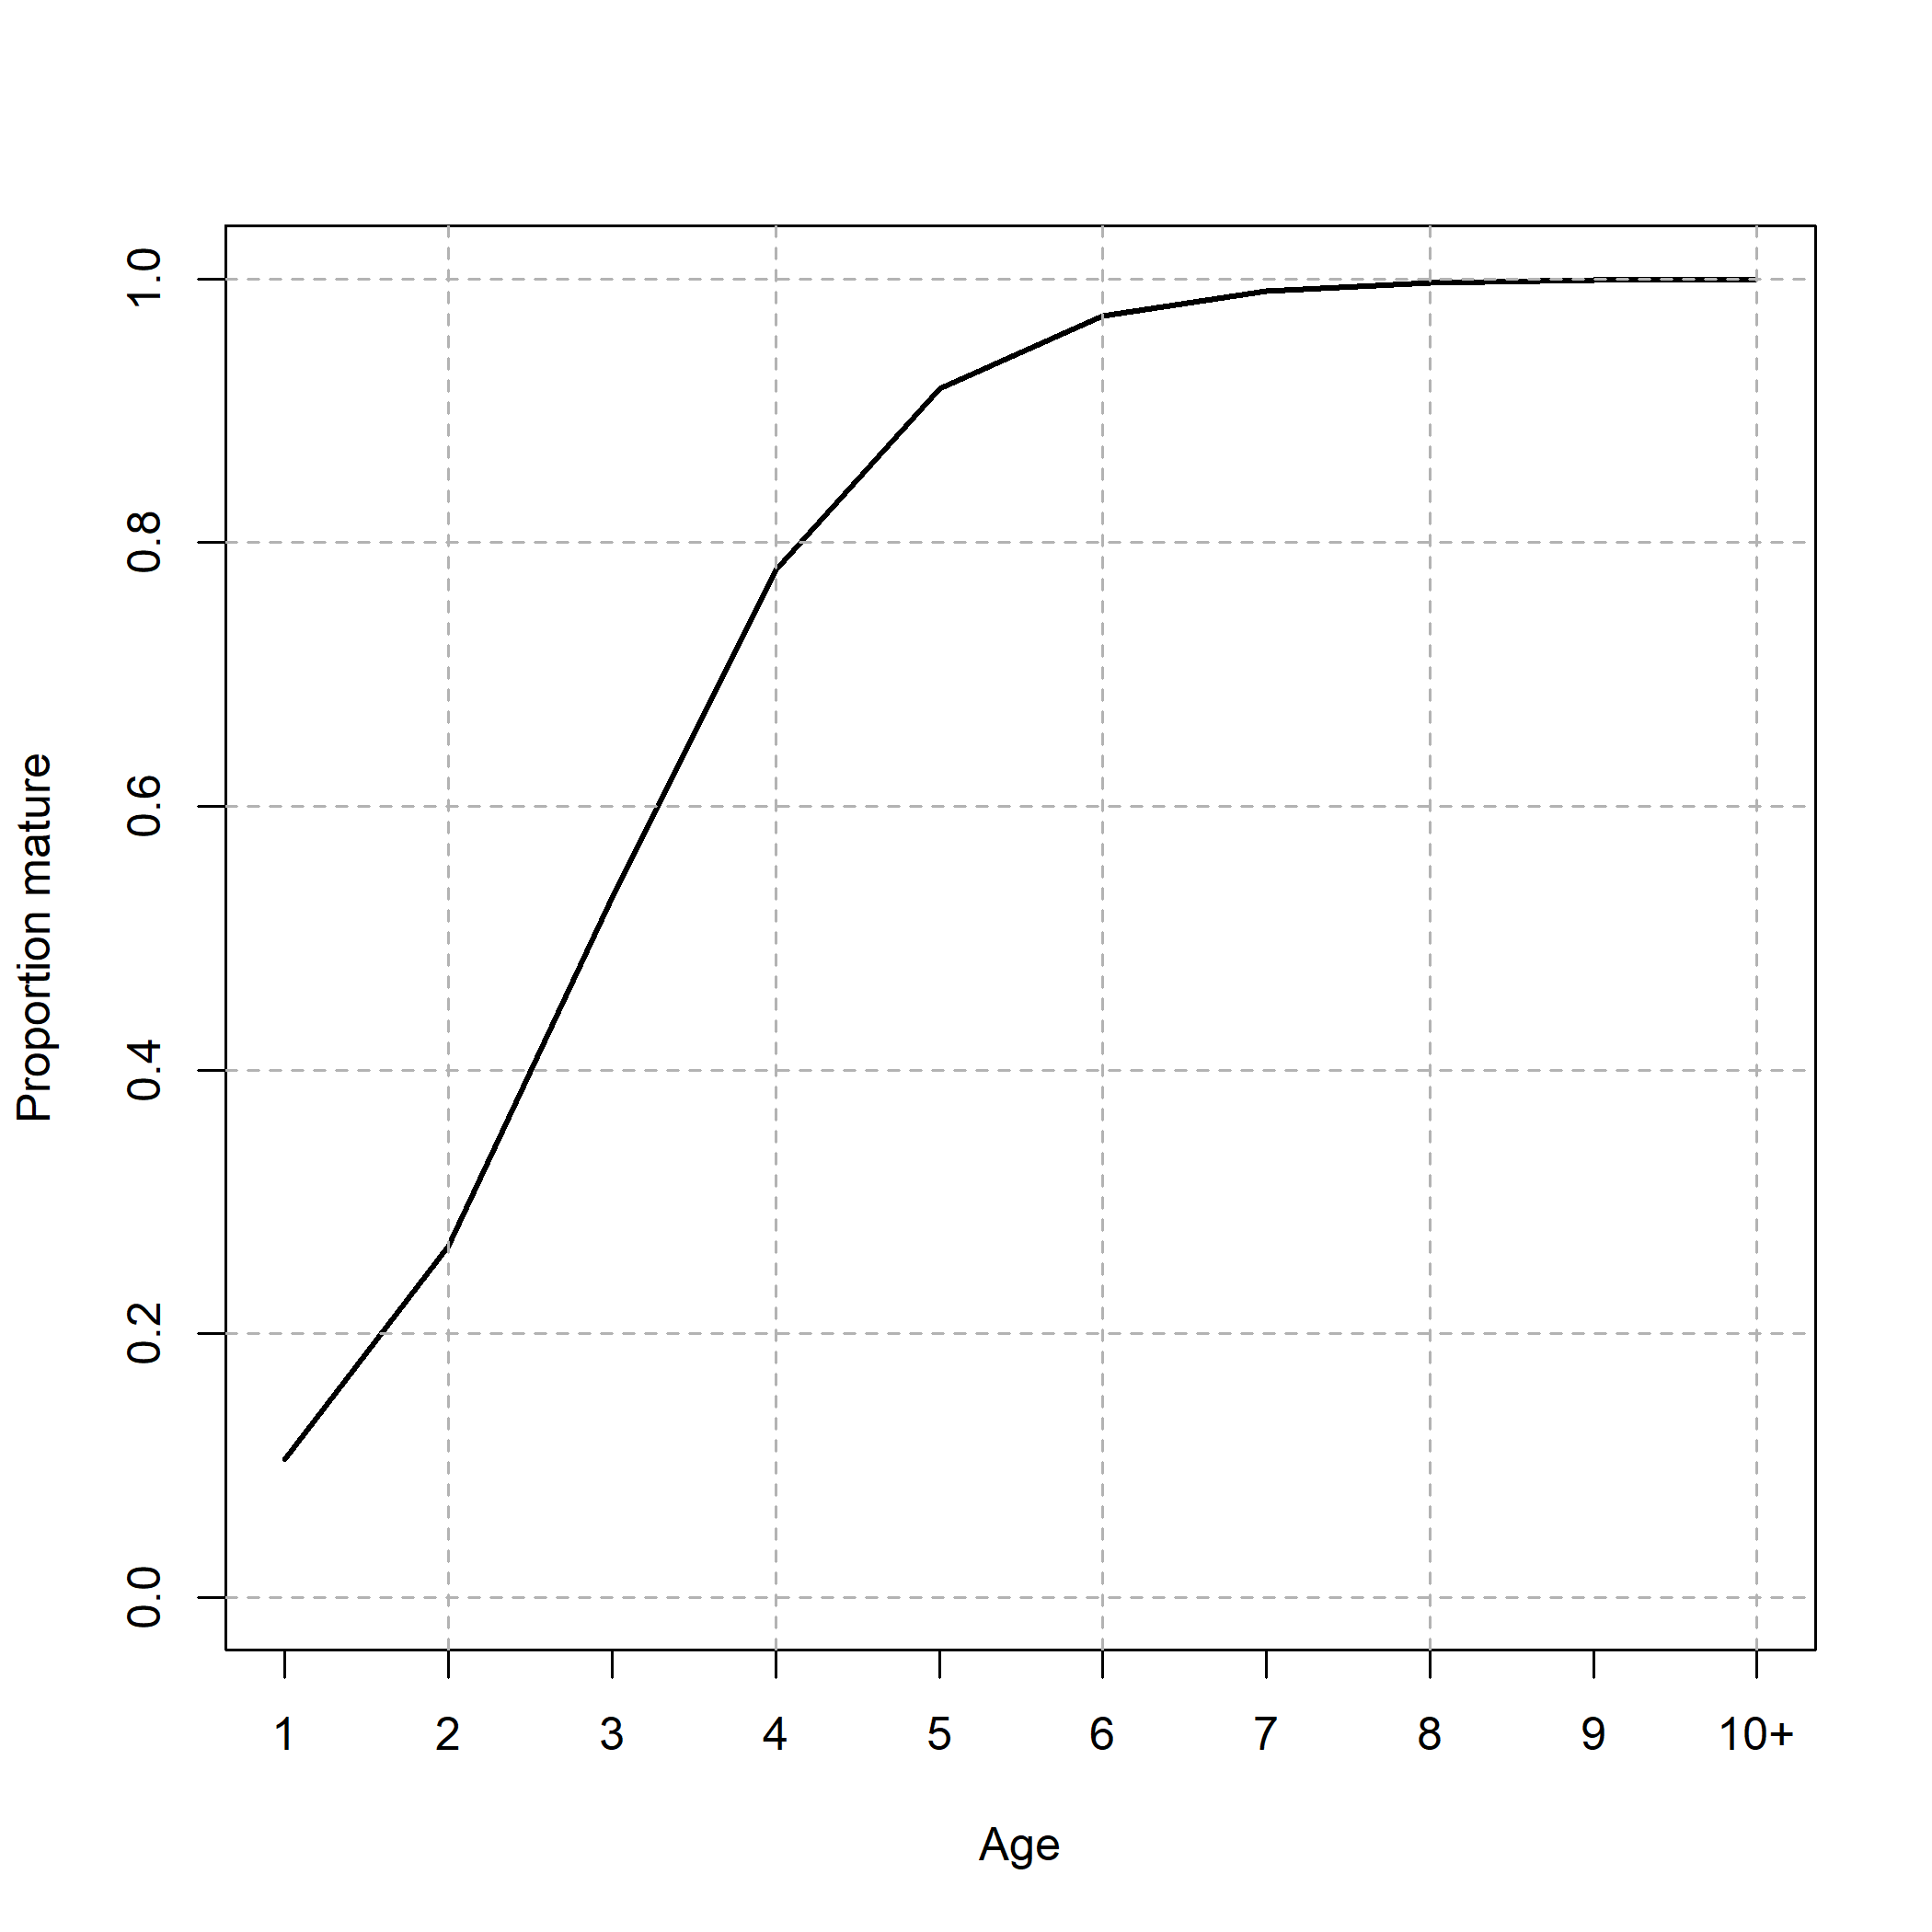
\includegraphics[width = \textwidth]{om_maturity.png}
\end{center}
\end{figure}

\begin{figure}
\caption{The weight at age assumed for the population in all operating and estimating models.}\label{om_waa}
\begin{center}
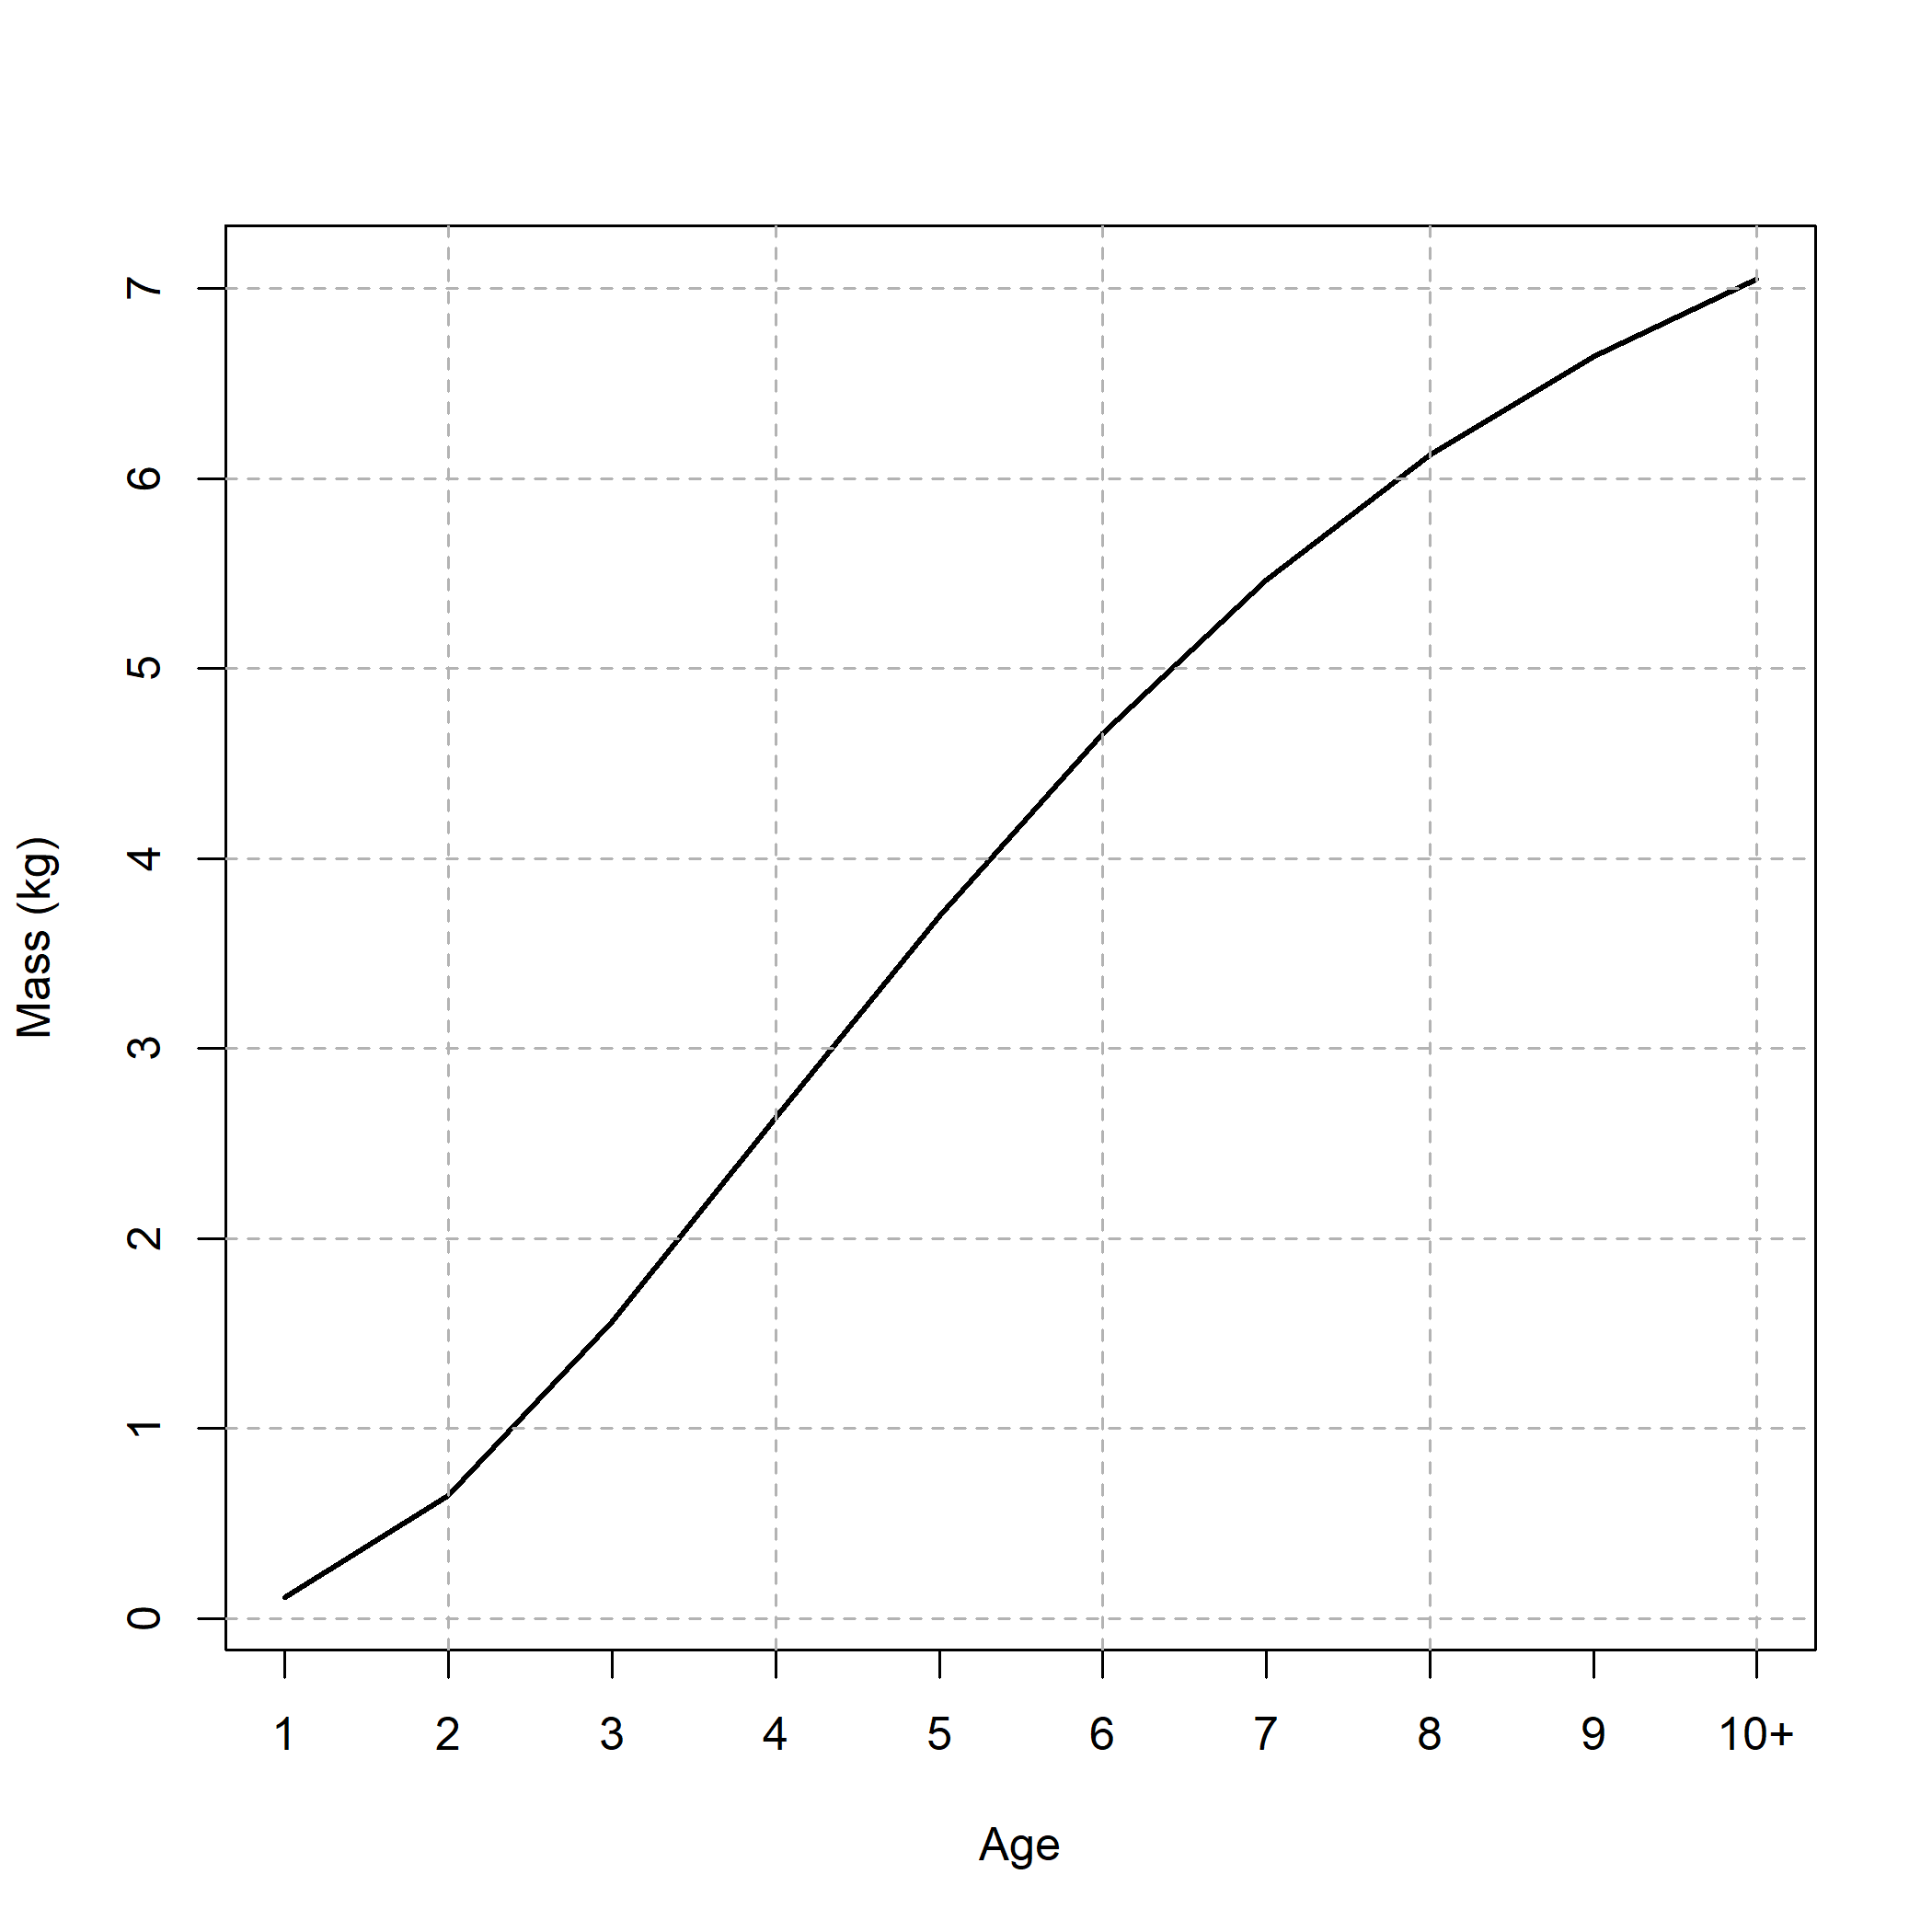
\includegraphics[width = \textwidth]{om_waa.png}
\end{center}
\end{figure}

\begin{figure}
\caption{The Beverton-Holt stock recruit relationship assume for all operating models.}\label{om_sr}
\begin{center}
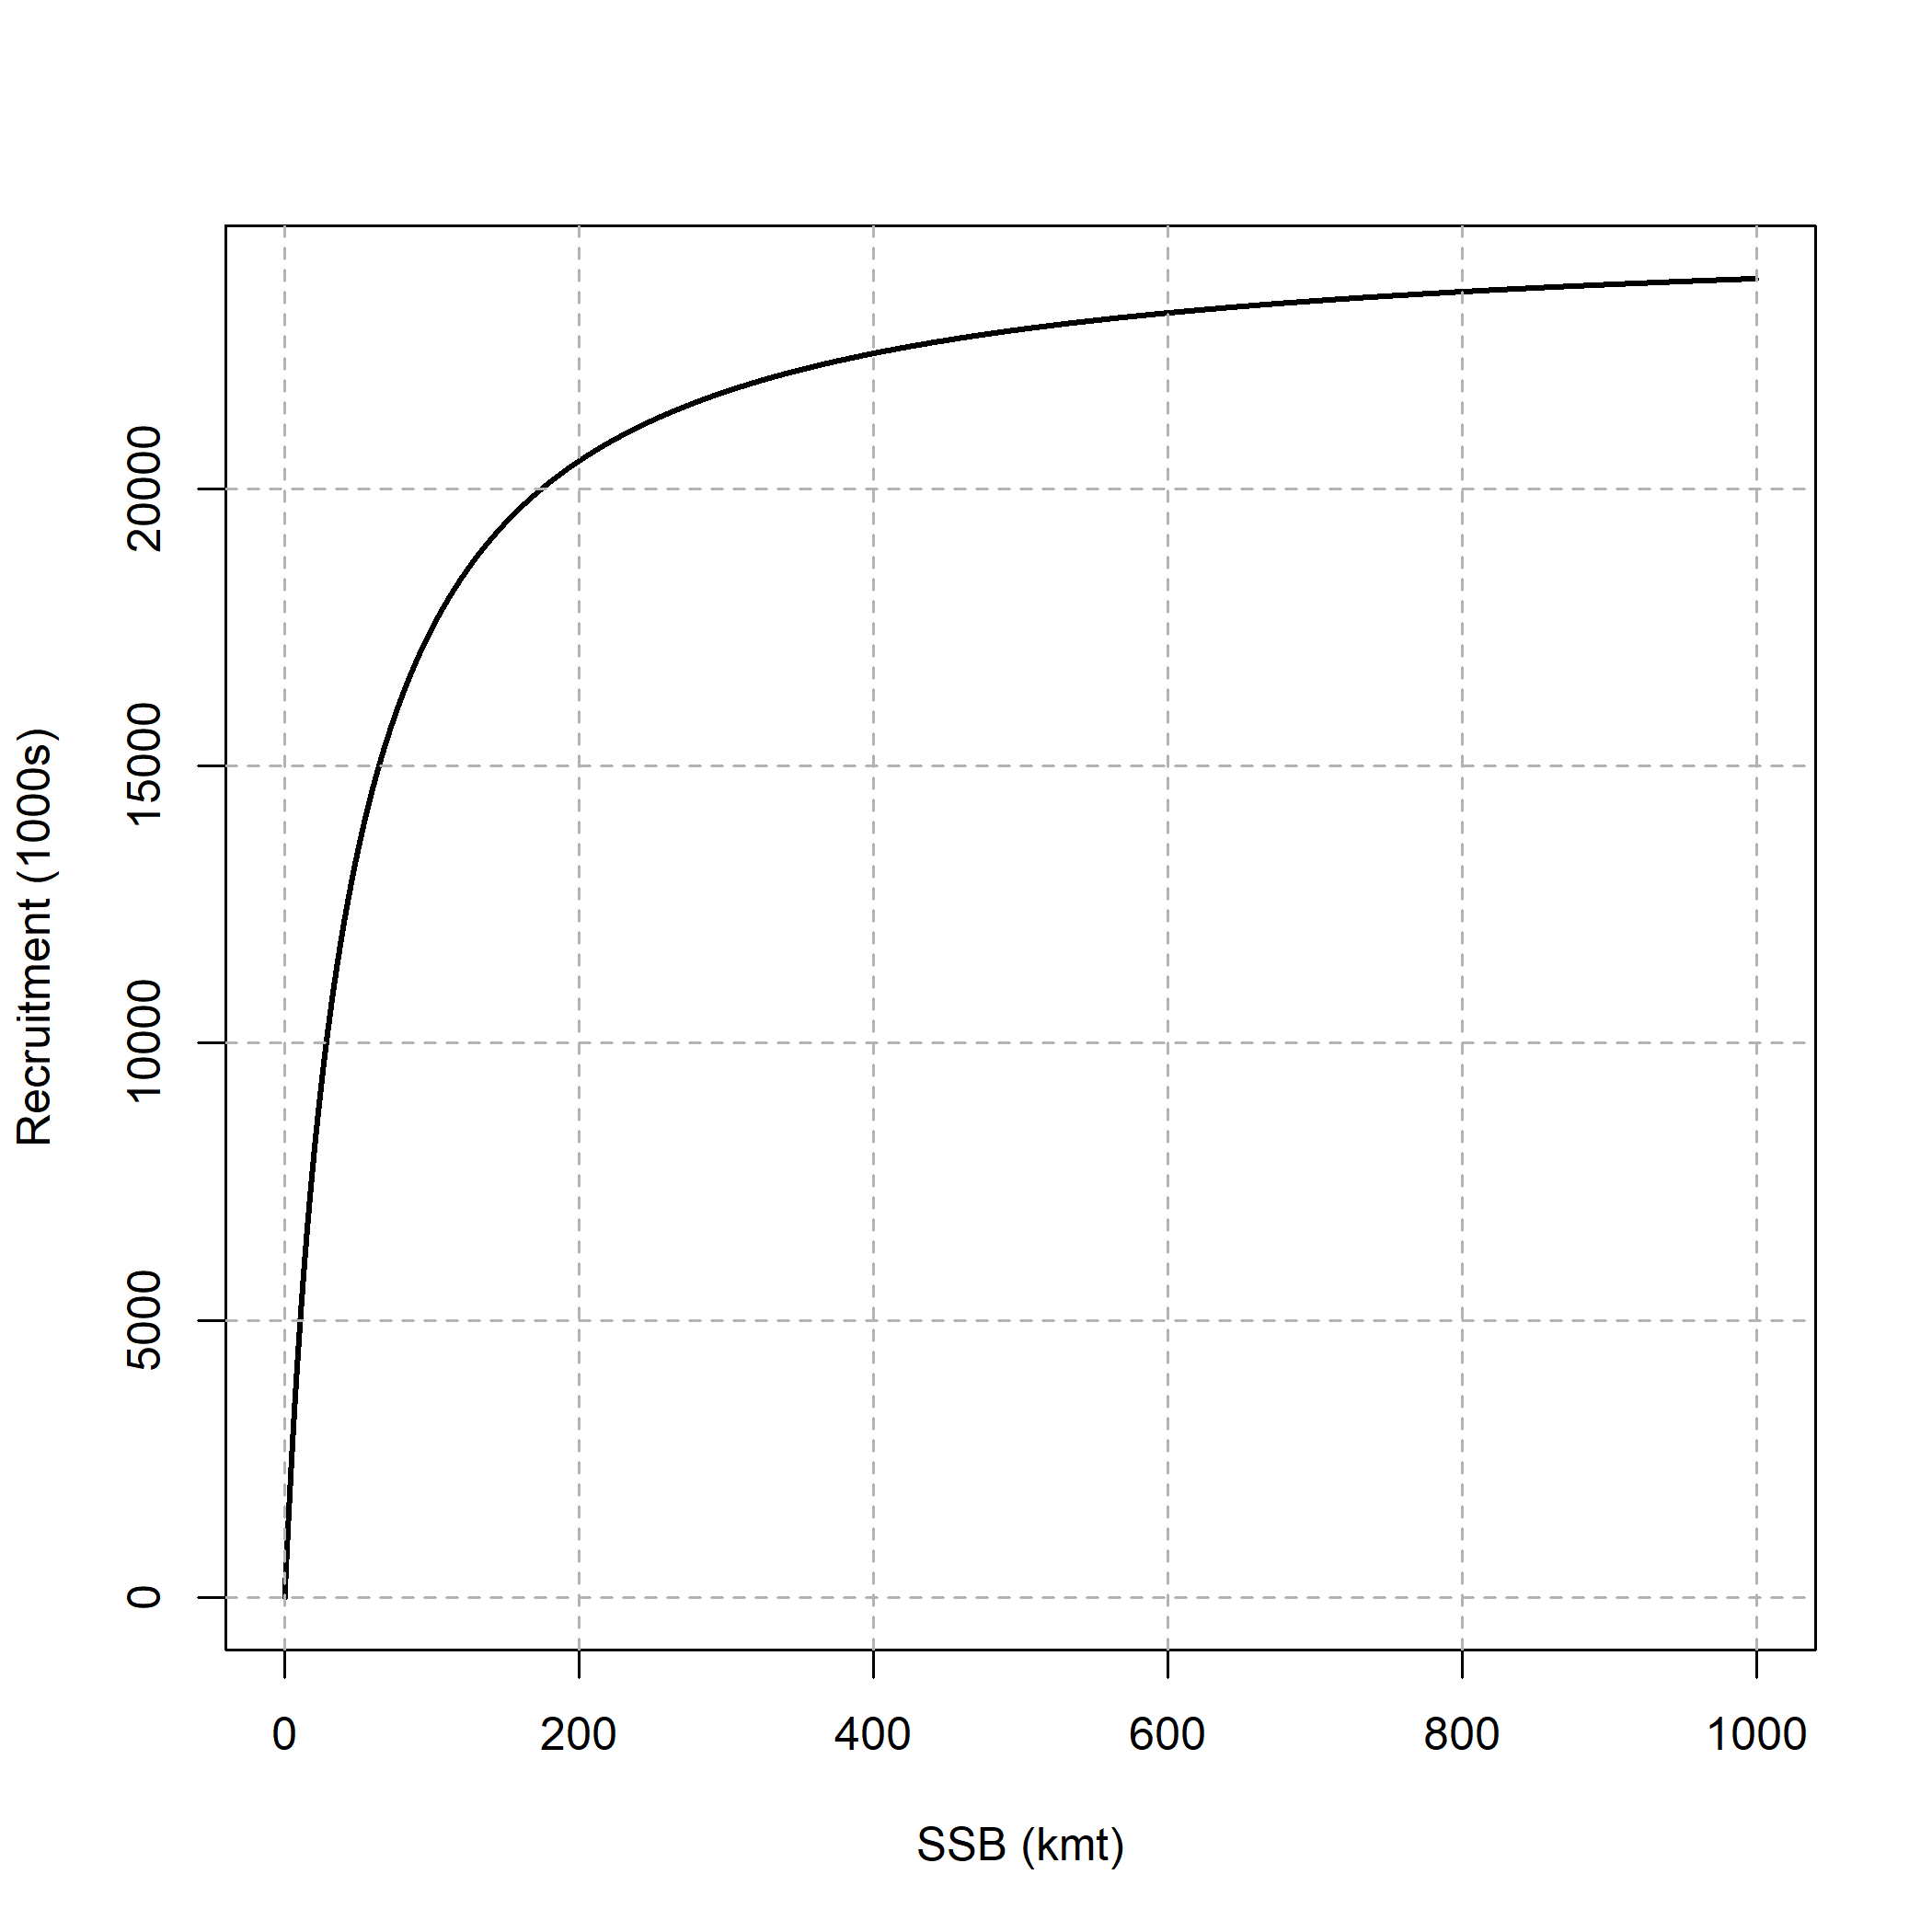
\includegraphics[width = \textwidth]{om_sr.png}
\end{center}
\end{figure}

\begin{figure}
\caption{Example simulations of environmental covariate latent processes and observations with different levels of observation error, and different assumptions about variability of the latent process.}\label{om_ecov_example}
\begin{center}
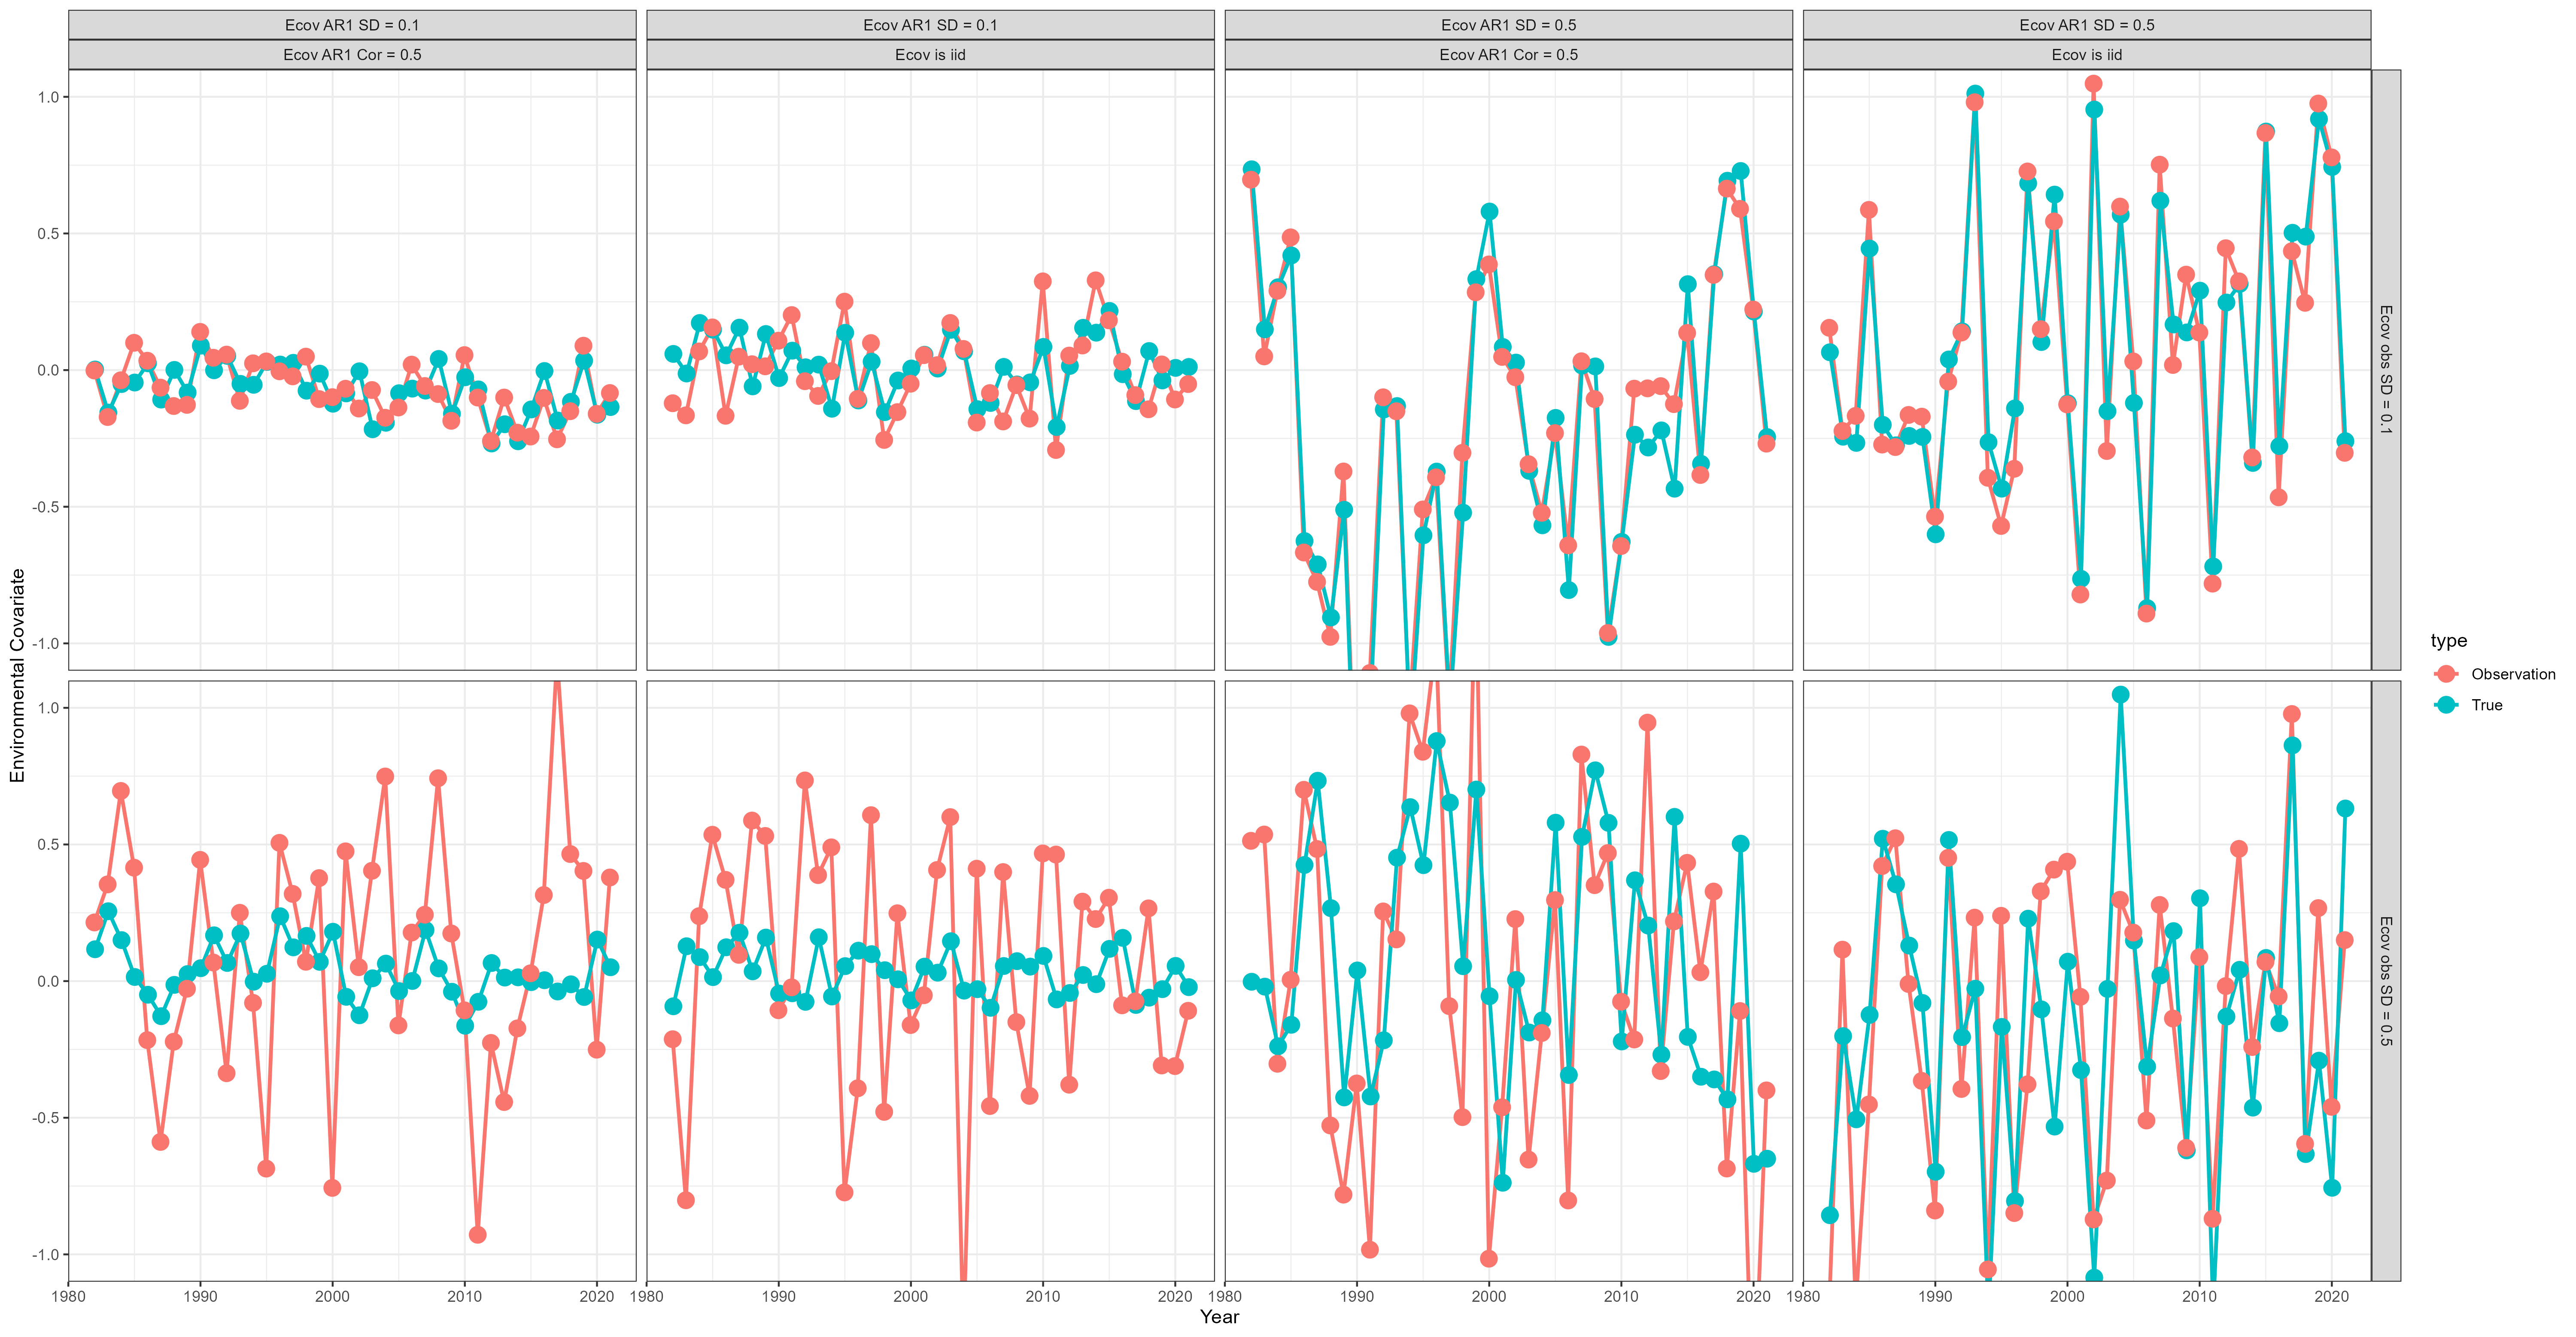
\includegraphics[width = \textwidth]{Ecov_true_obs_example.png}
\end{center}
\end{figure}

\begin{landscape}
\begin{figure}
\caption{Example simulations of annual natural mortality rates that may be a function of a temporally varying environmental covariate and autoregressive random effects.}\label{M_example}
\begin{center}
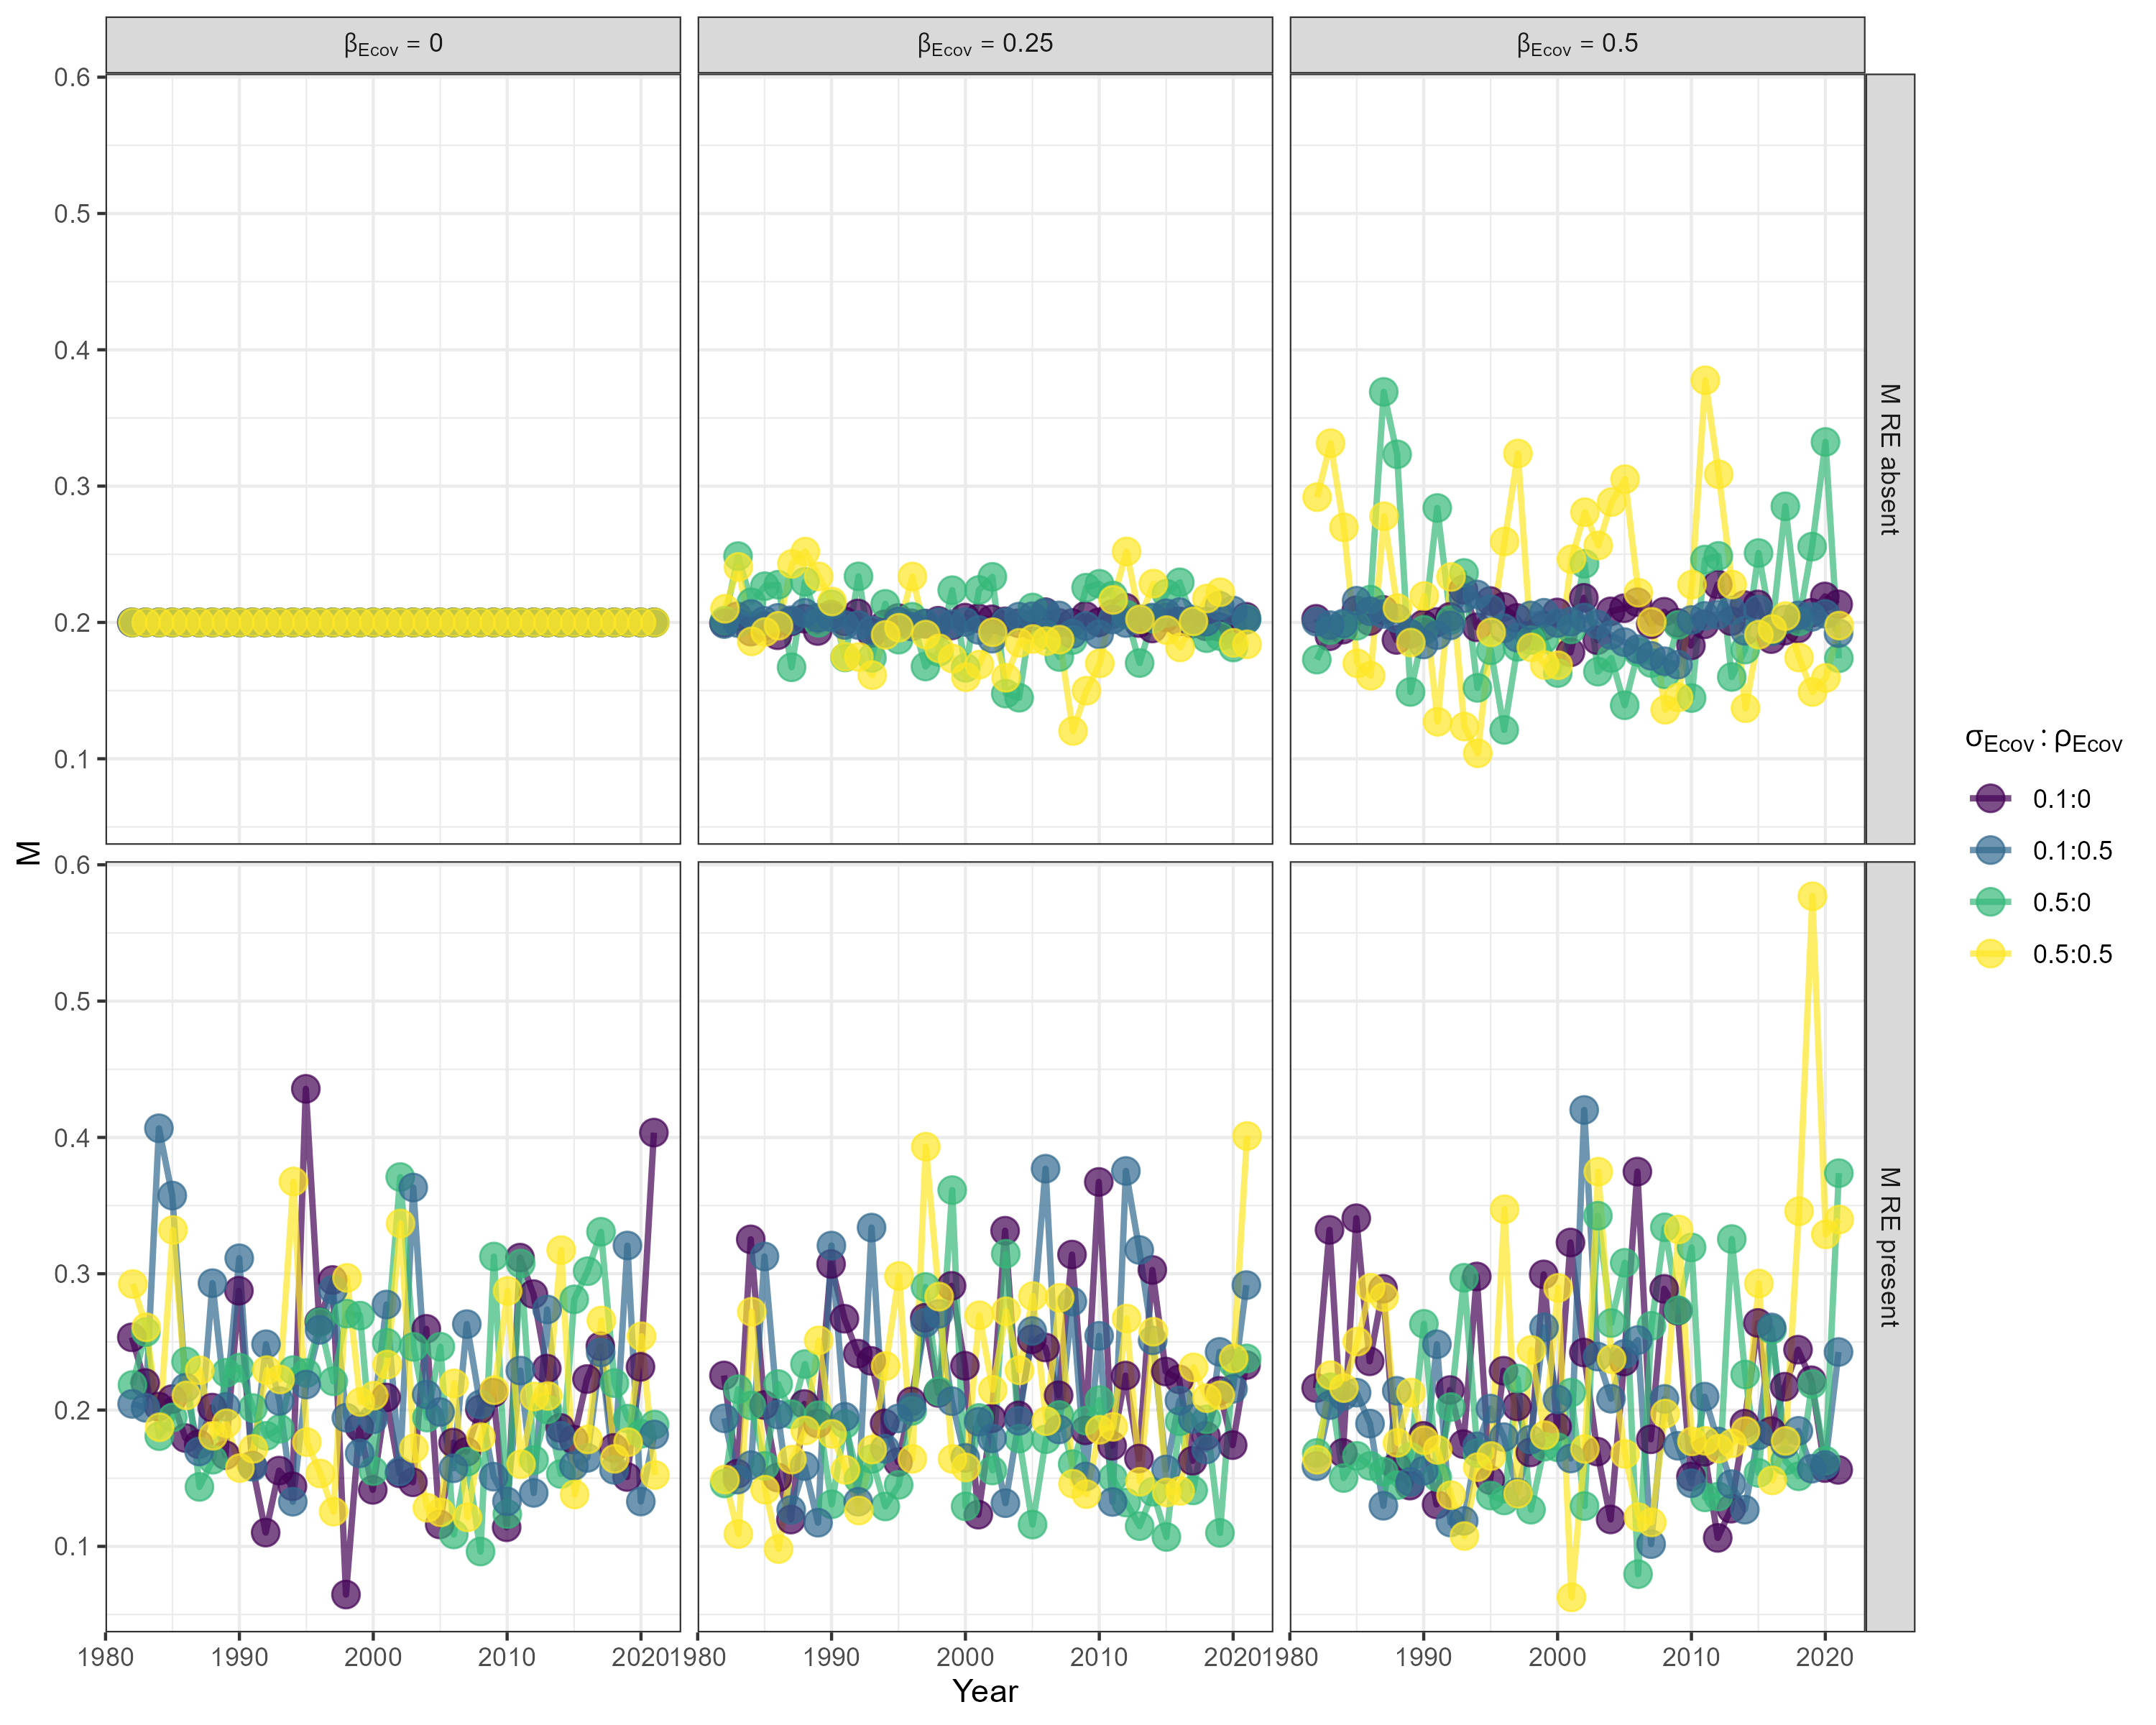
\includegraphics[width = \textwidth]{M_example.png}
\end{center}
\end{figure}
\end{landscape}

\begin{figure}
\caption{The selectivity at age assumed for the fishing fleet in operating models without selectivity random effects. The mean selectivity at age across time for the fishing fleet in operating models with selectivity random effects.}\label{om_mean_selectivity}
\begin{center}
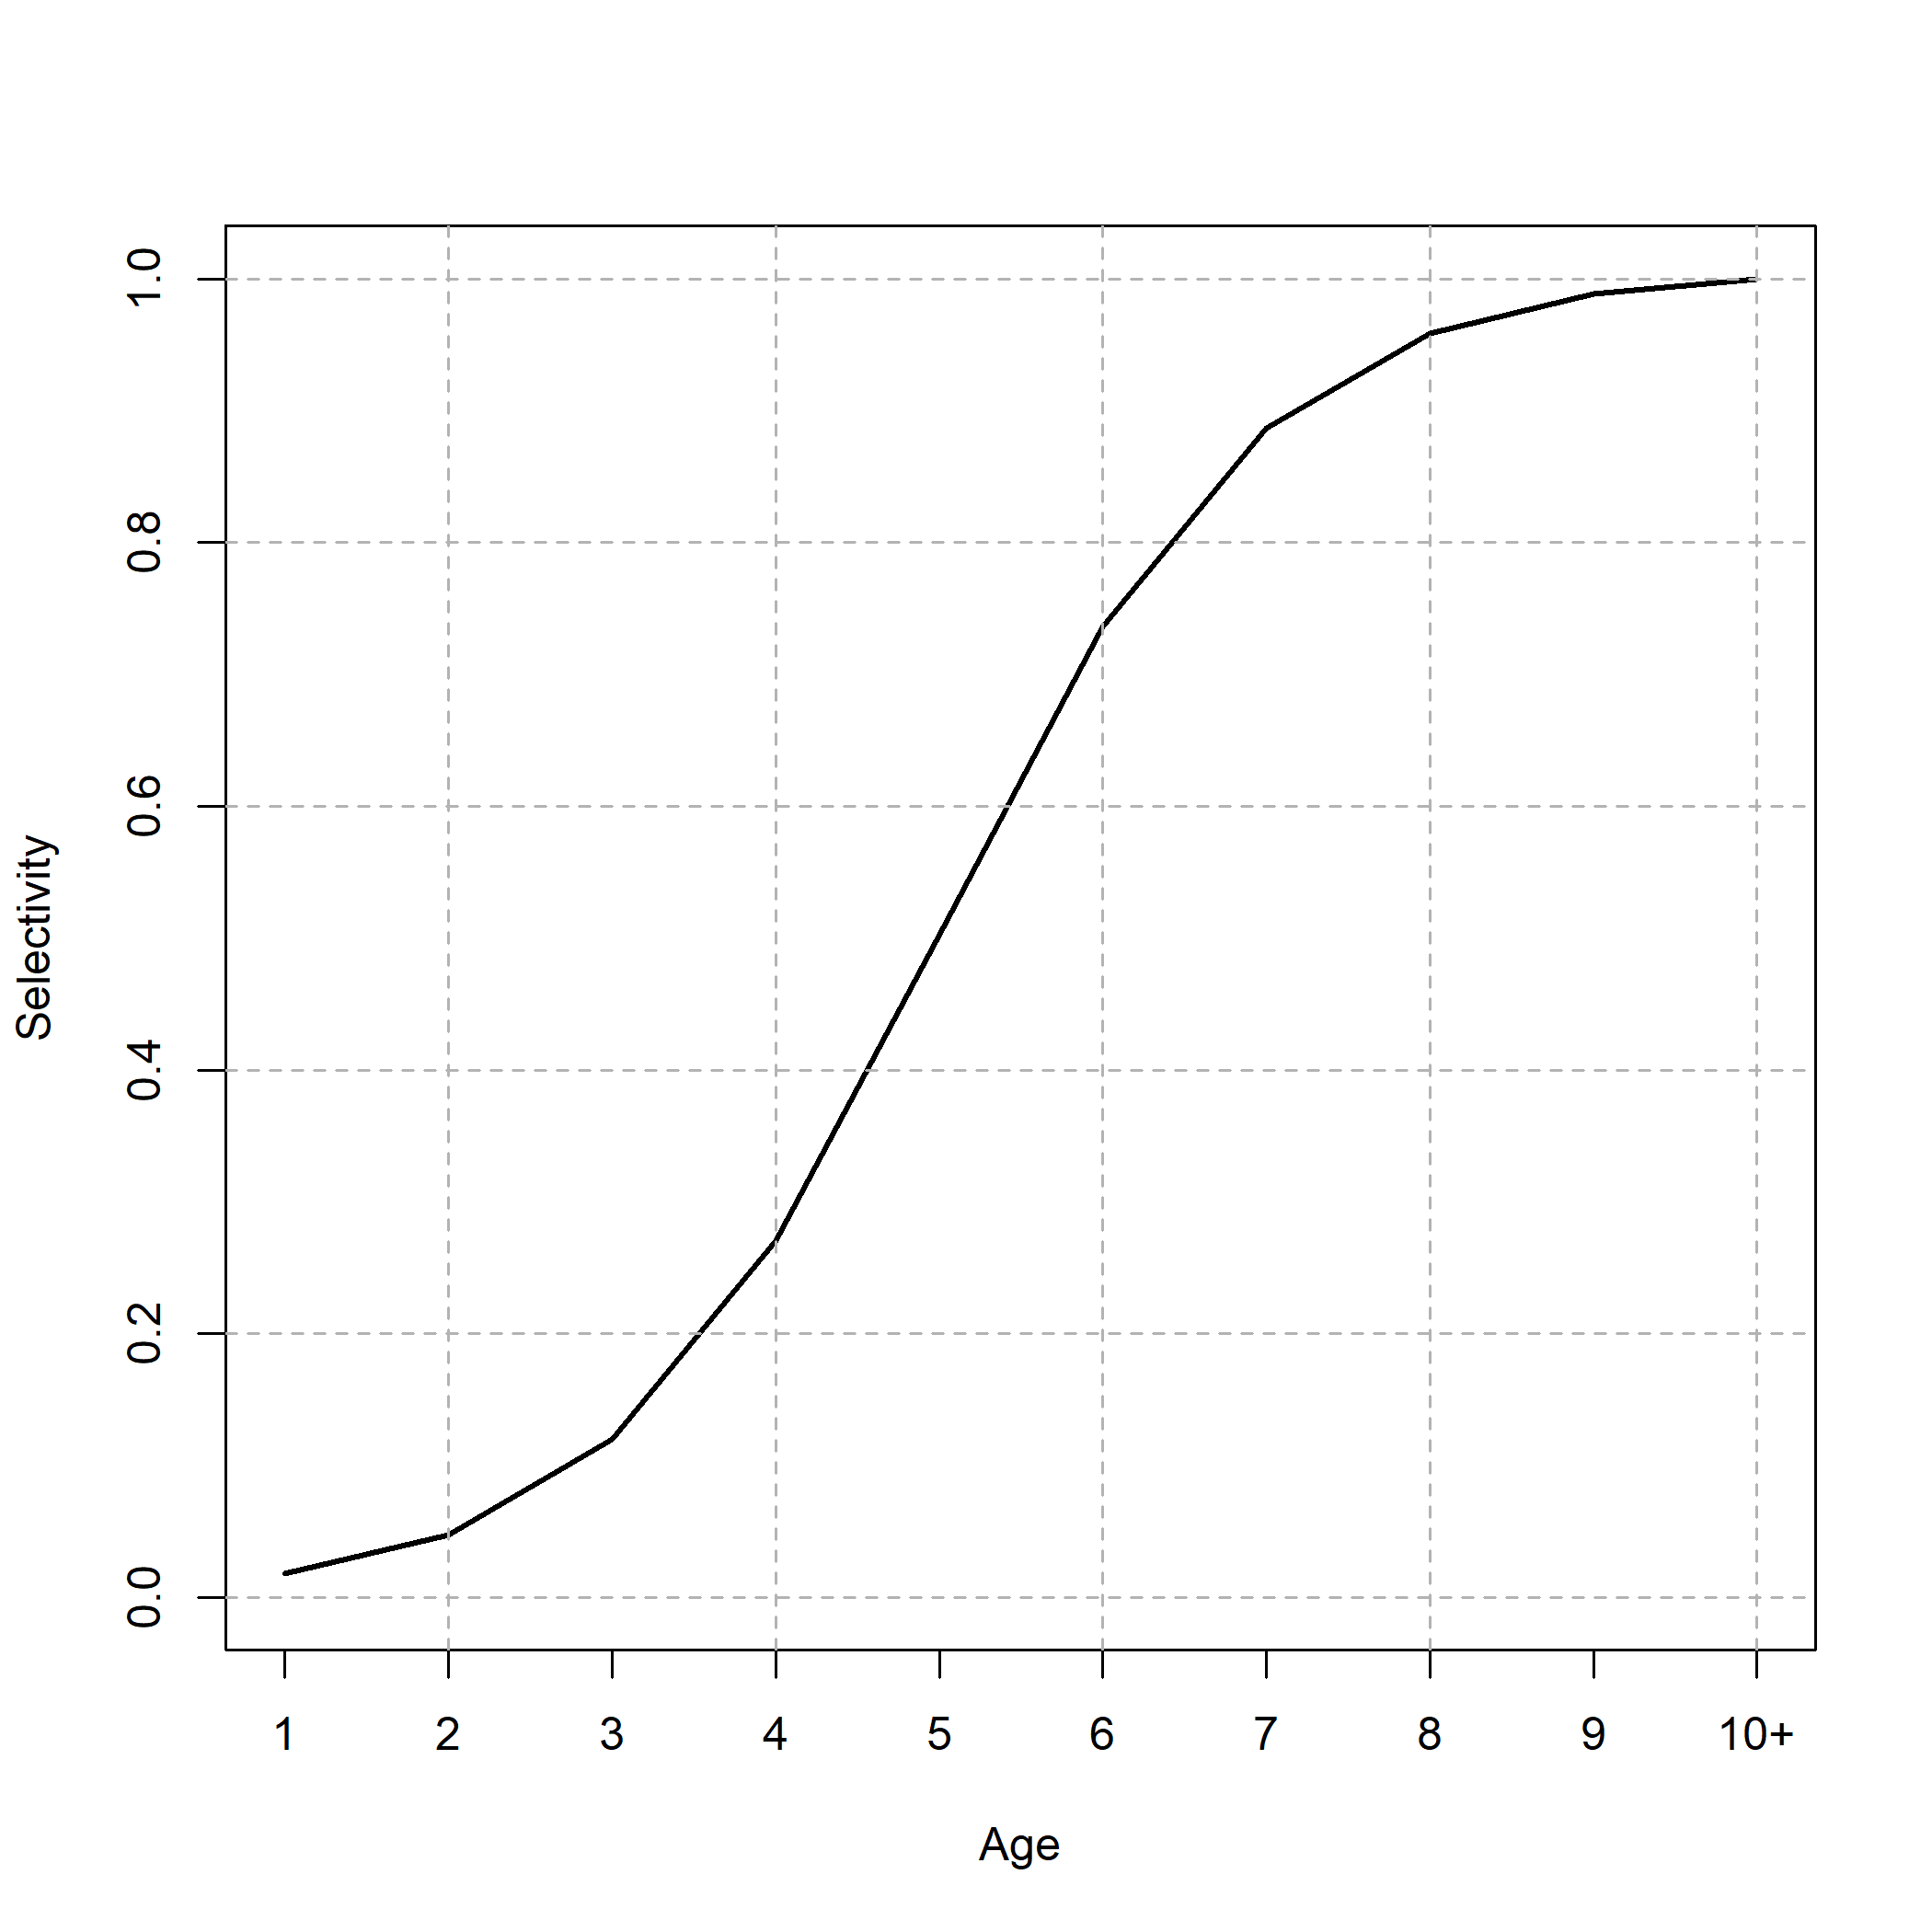
\includegraphics[width = \textwidth]{om_mean_selectivity.png}
\end{center}
\end{figure}

\begin{landscape}
\begin{figure}
\caption{Probability of convergence of estimating models with alternative process error assumptions fit to simulated populations and data sets from operating models. The convergence criterion is an invertible hessian providing standard error estimates for all fixed effects parameters. Vertical lines represent 95\% confidence intervals. All estimating models estimate environmental covariate effects on natural mortality but assume the mean mortality parameter $\beta_\text{M} = \log 0.2$.}\label{convergence_M_fixed}
\begin{center}
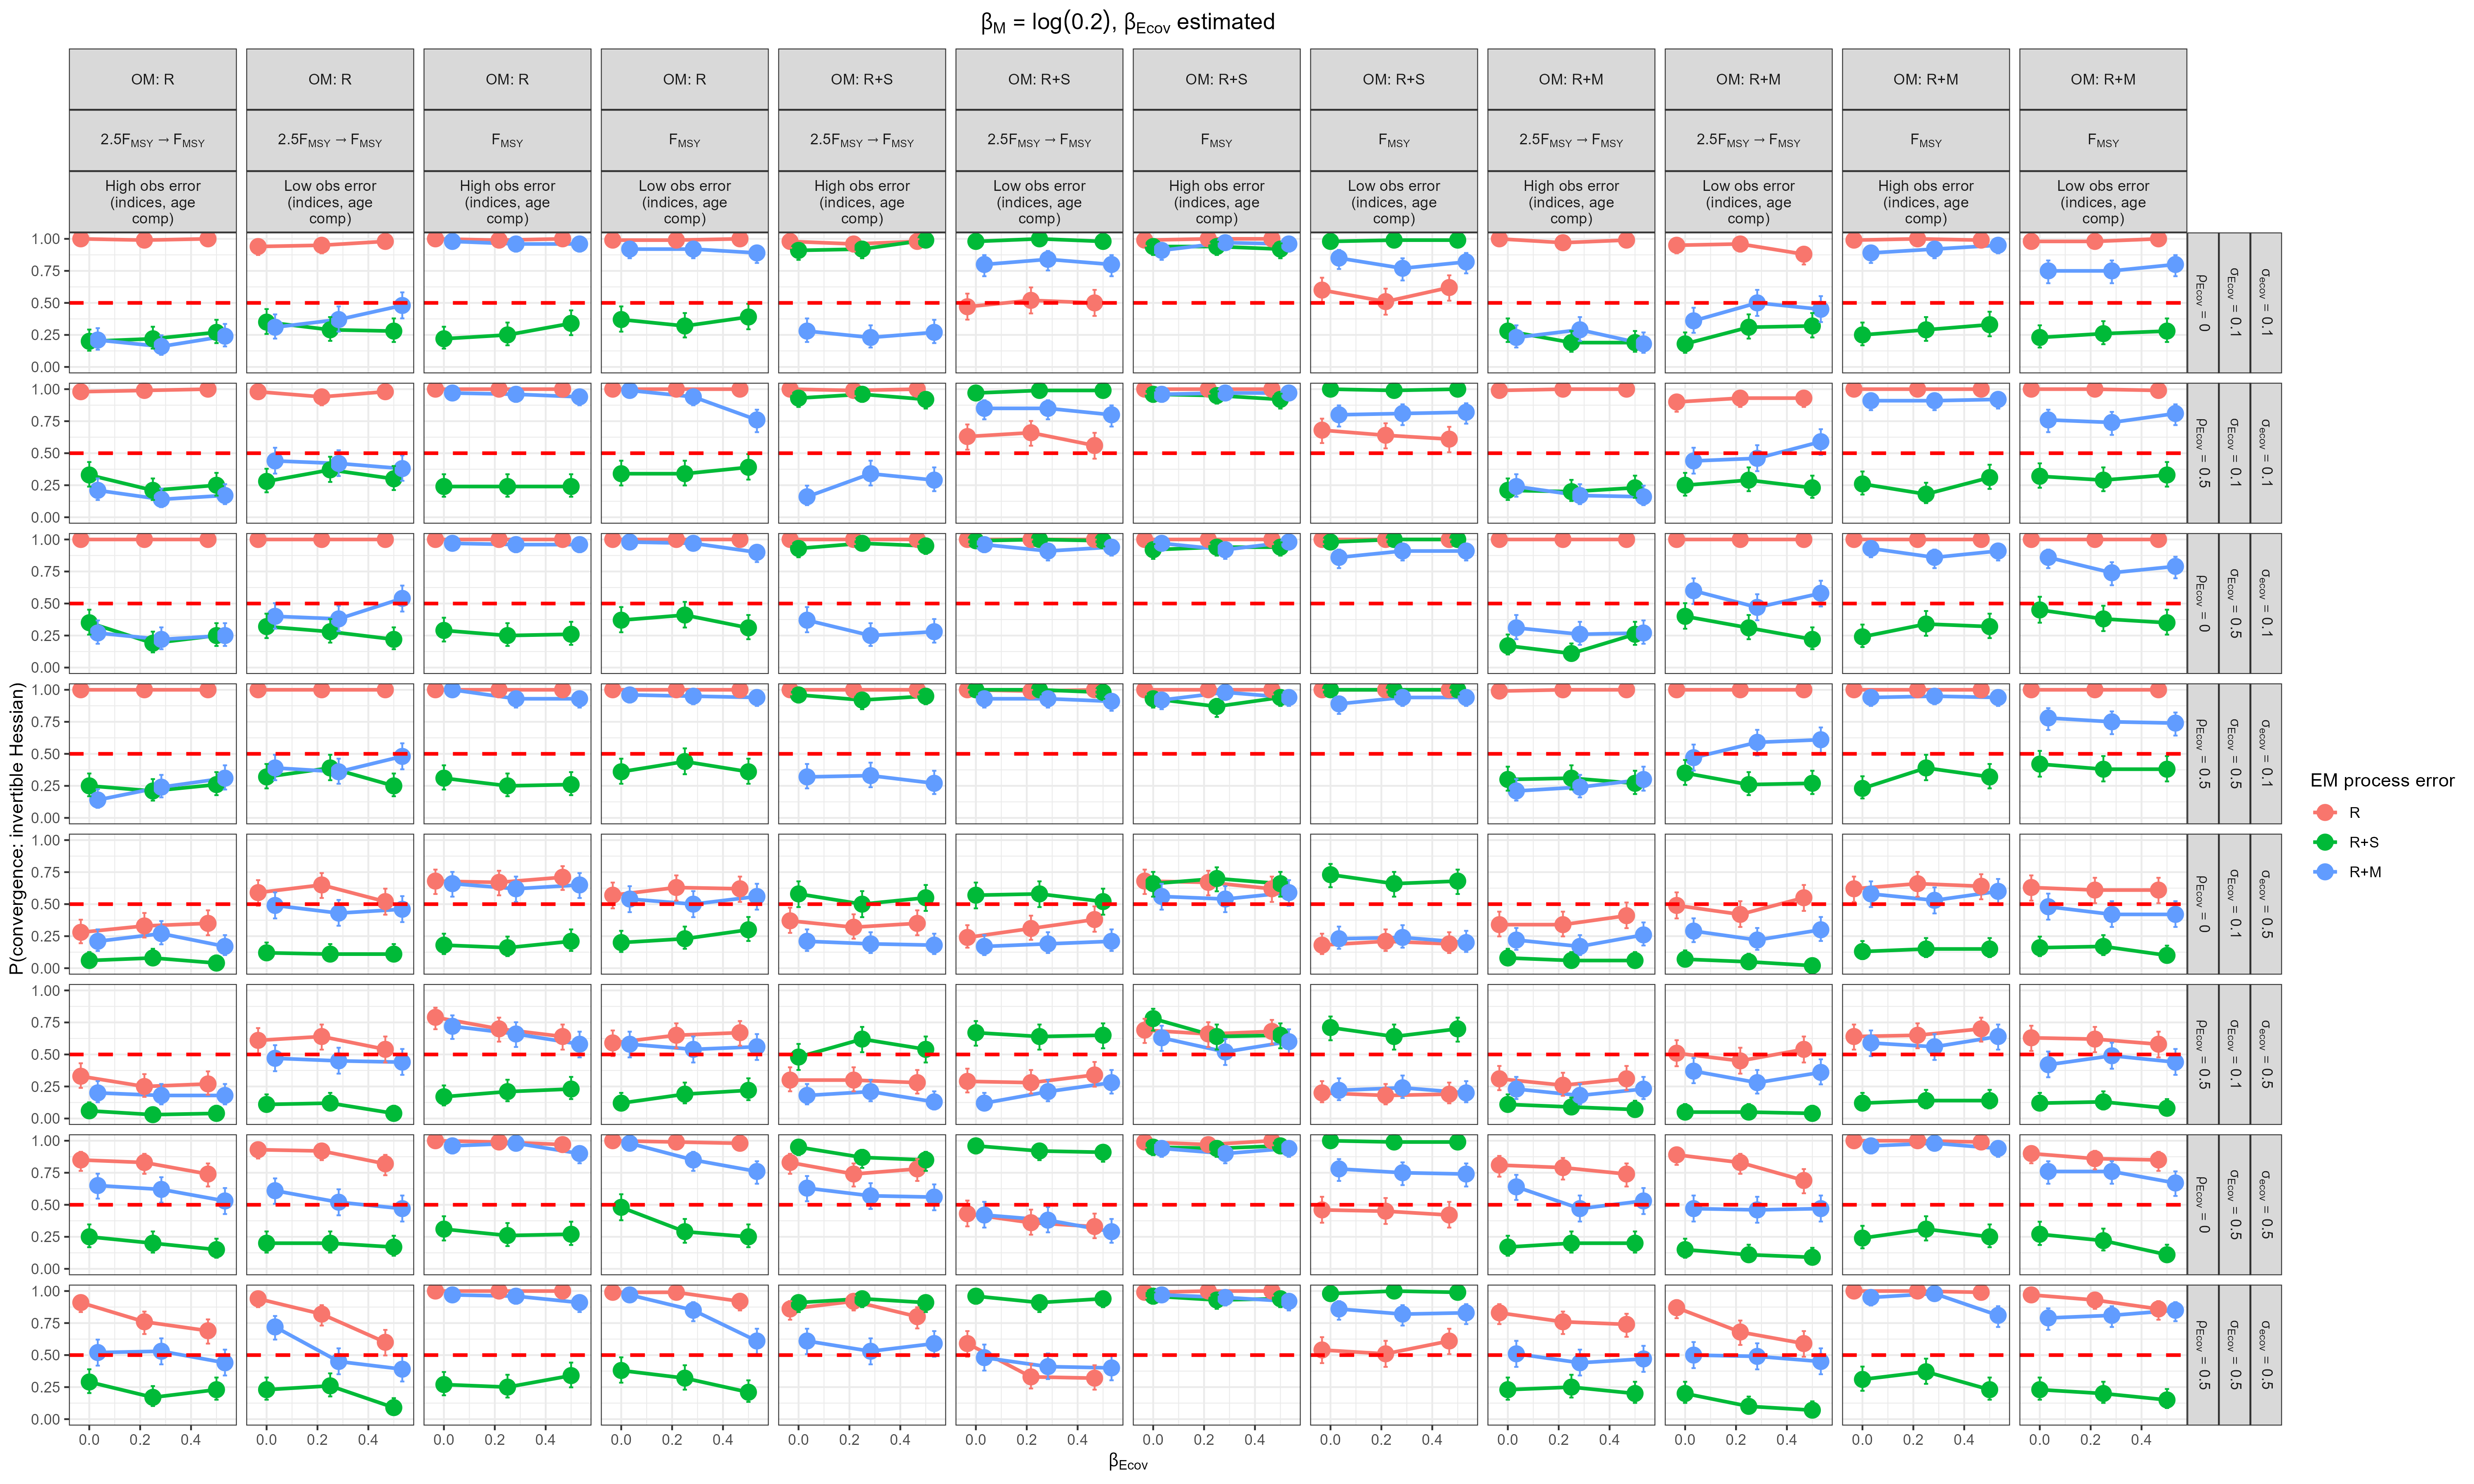
\includegraphics[height = \textheight]{proportion_good_hessian_ecov_effect_est_M_fixed.png}
\end{center}
\end{figure}
\end{landscape}

\begin{landscape}
\begin{figure}
\caption{Probability of convergence of estimating models with alternative process error assumptions fit to simulated populations and data sets from operating models. The convergence criterion is an invertible hessian providing standard error estimates for all fixed effects parameters. Vertical lines represent 95\% confidence intervals. All estimating models estimate environmental covariate effects on natural mortality and the mean mortality parameter $\beta_\text{M}$.}\label{convergence_M_estimated}
\begin{center}
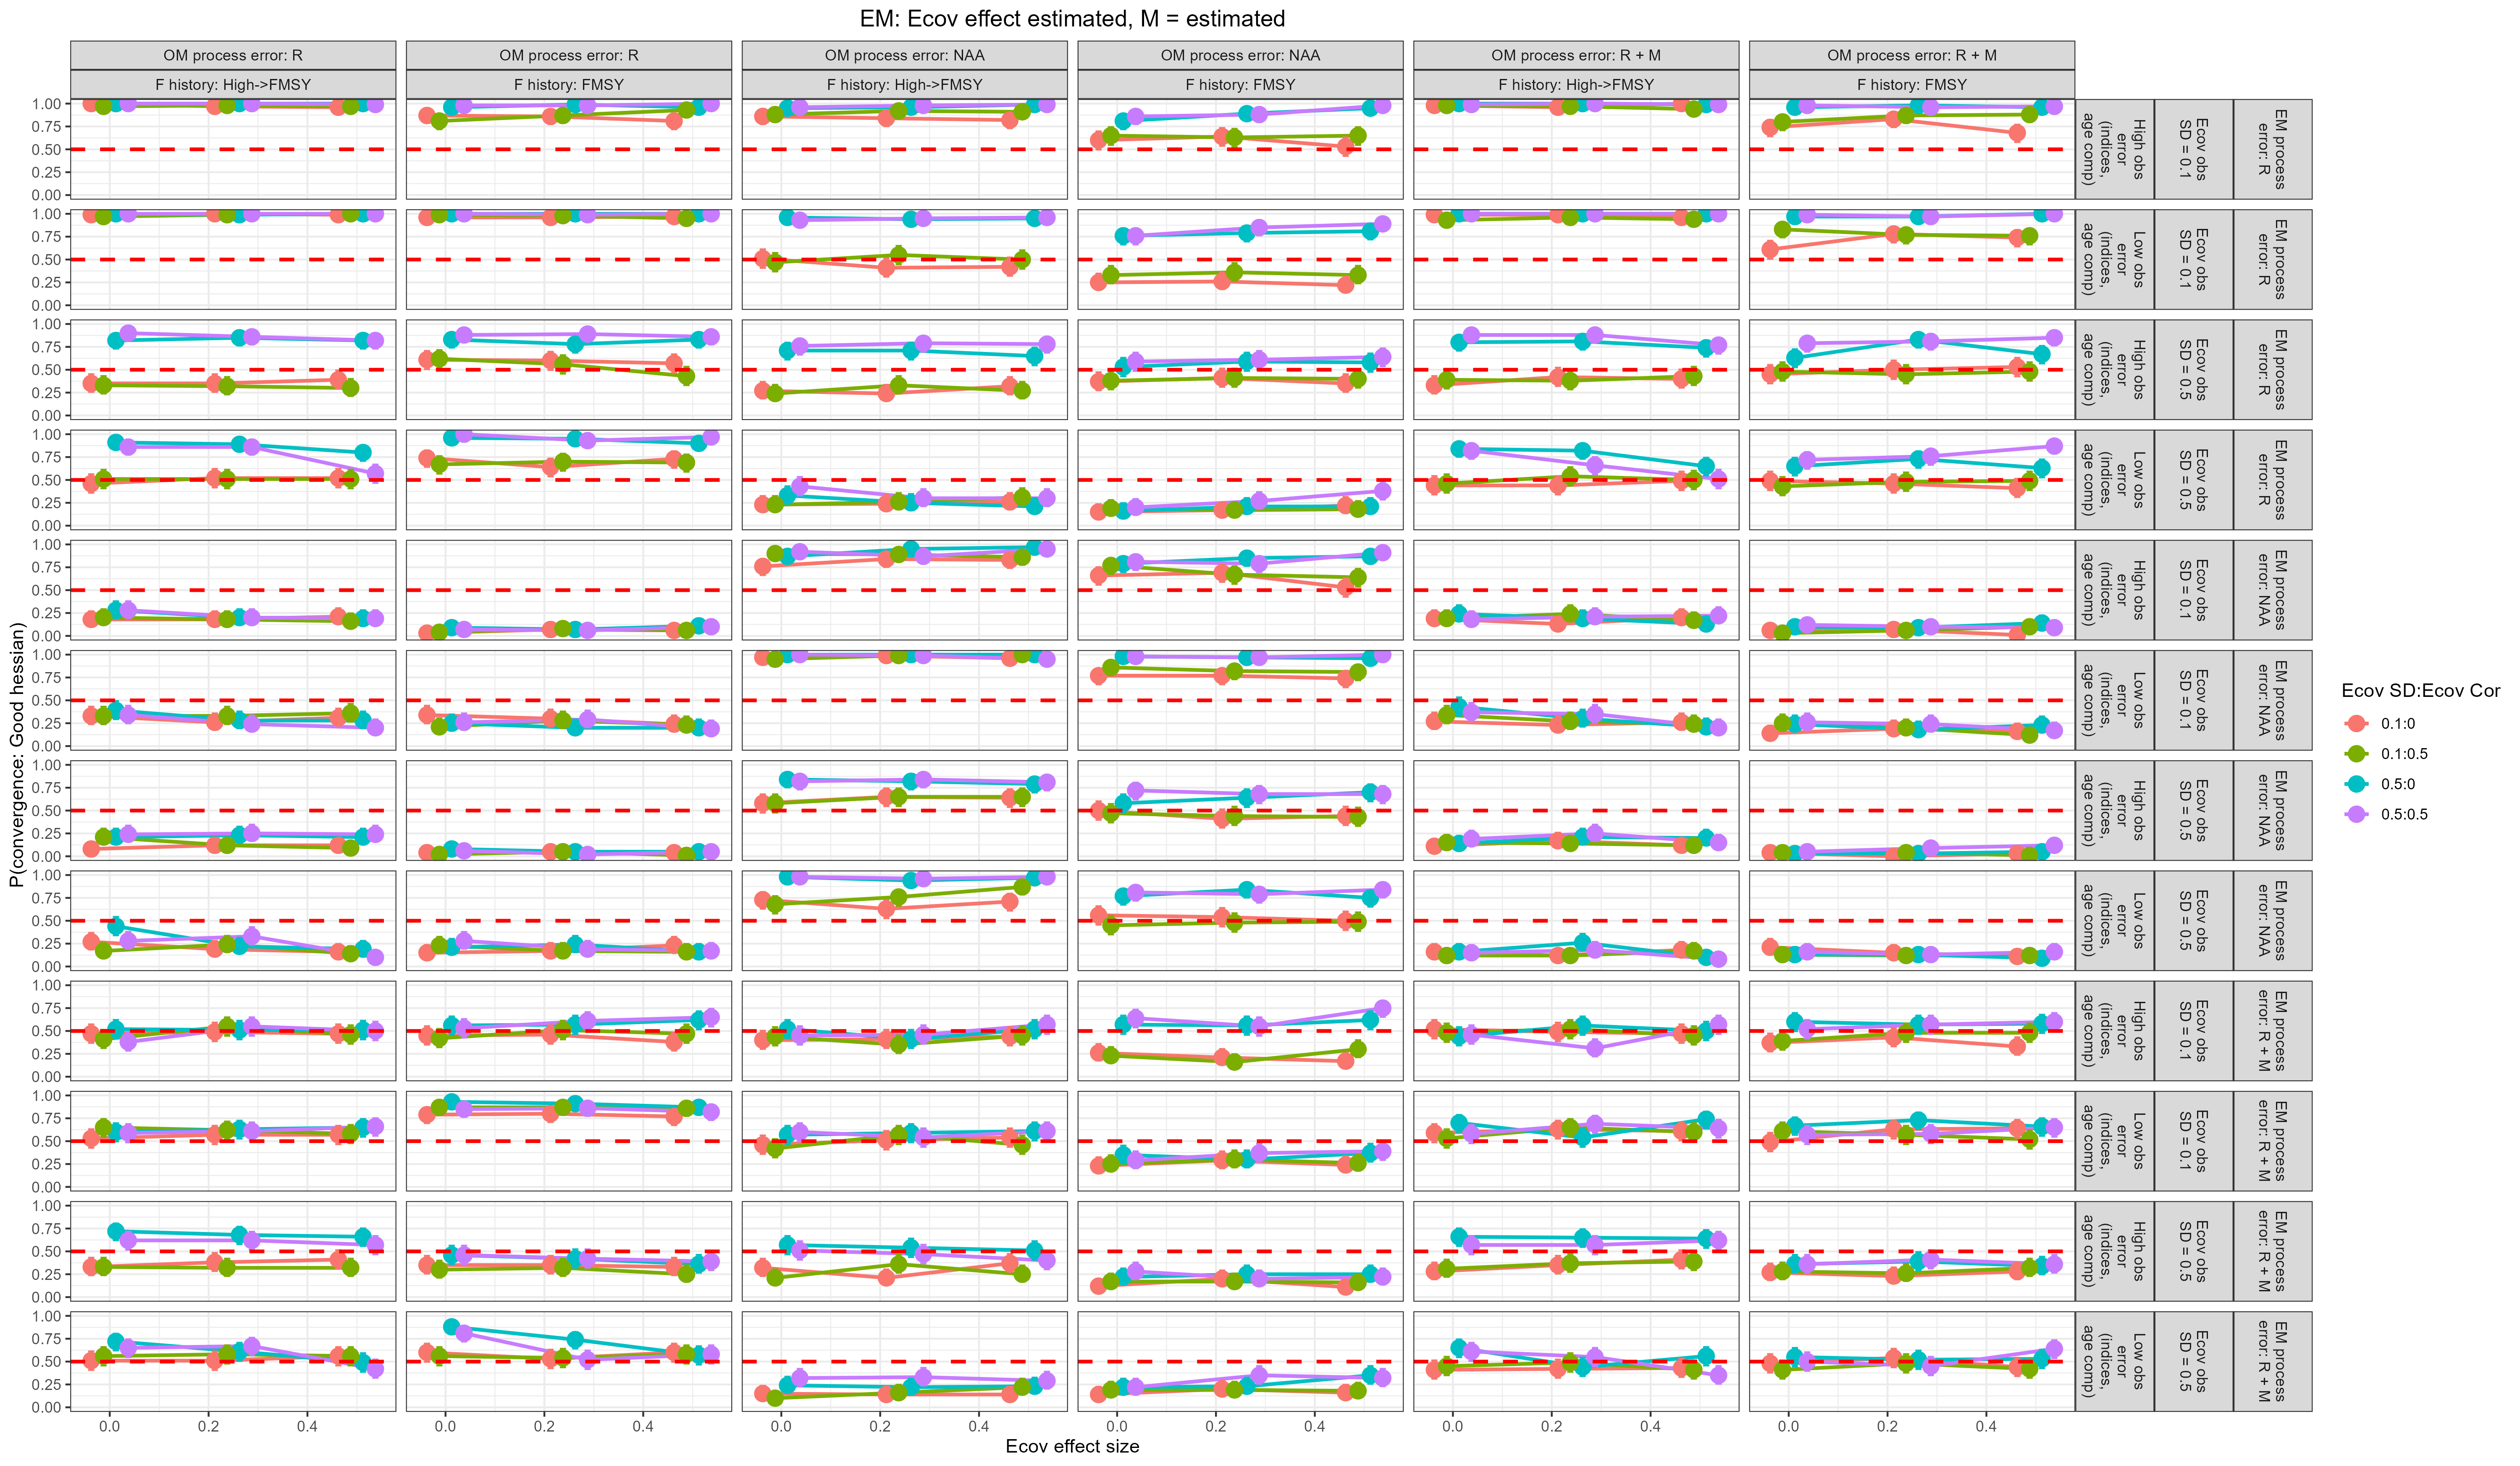
\includegraphics[height = \textheight]{proportion_good_hessian_ecov_effect_est_M_est.png}
\end{center}
\end{figure}
\end{landscape}

\begin{landscape}
\begin{figure}
\caption{Proportion of simulated data sets for each operating model where the estimation model type (process error and covariate effect assumptions) had the lowest AIC. All estimating models assumed the mean mortality parameter $\beta_\text{M} = \log 0.2$.}\label{aic_rank_M_fixed}
\begin{center}
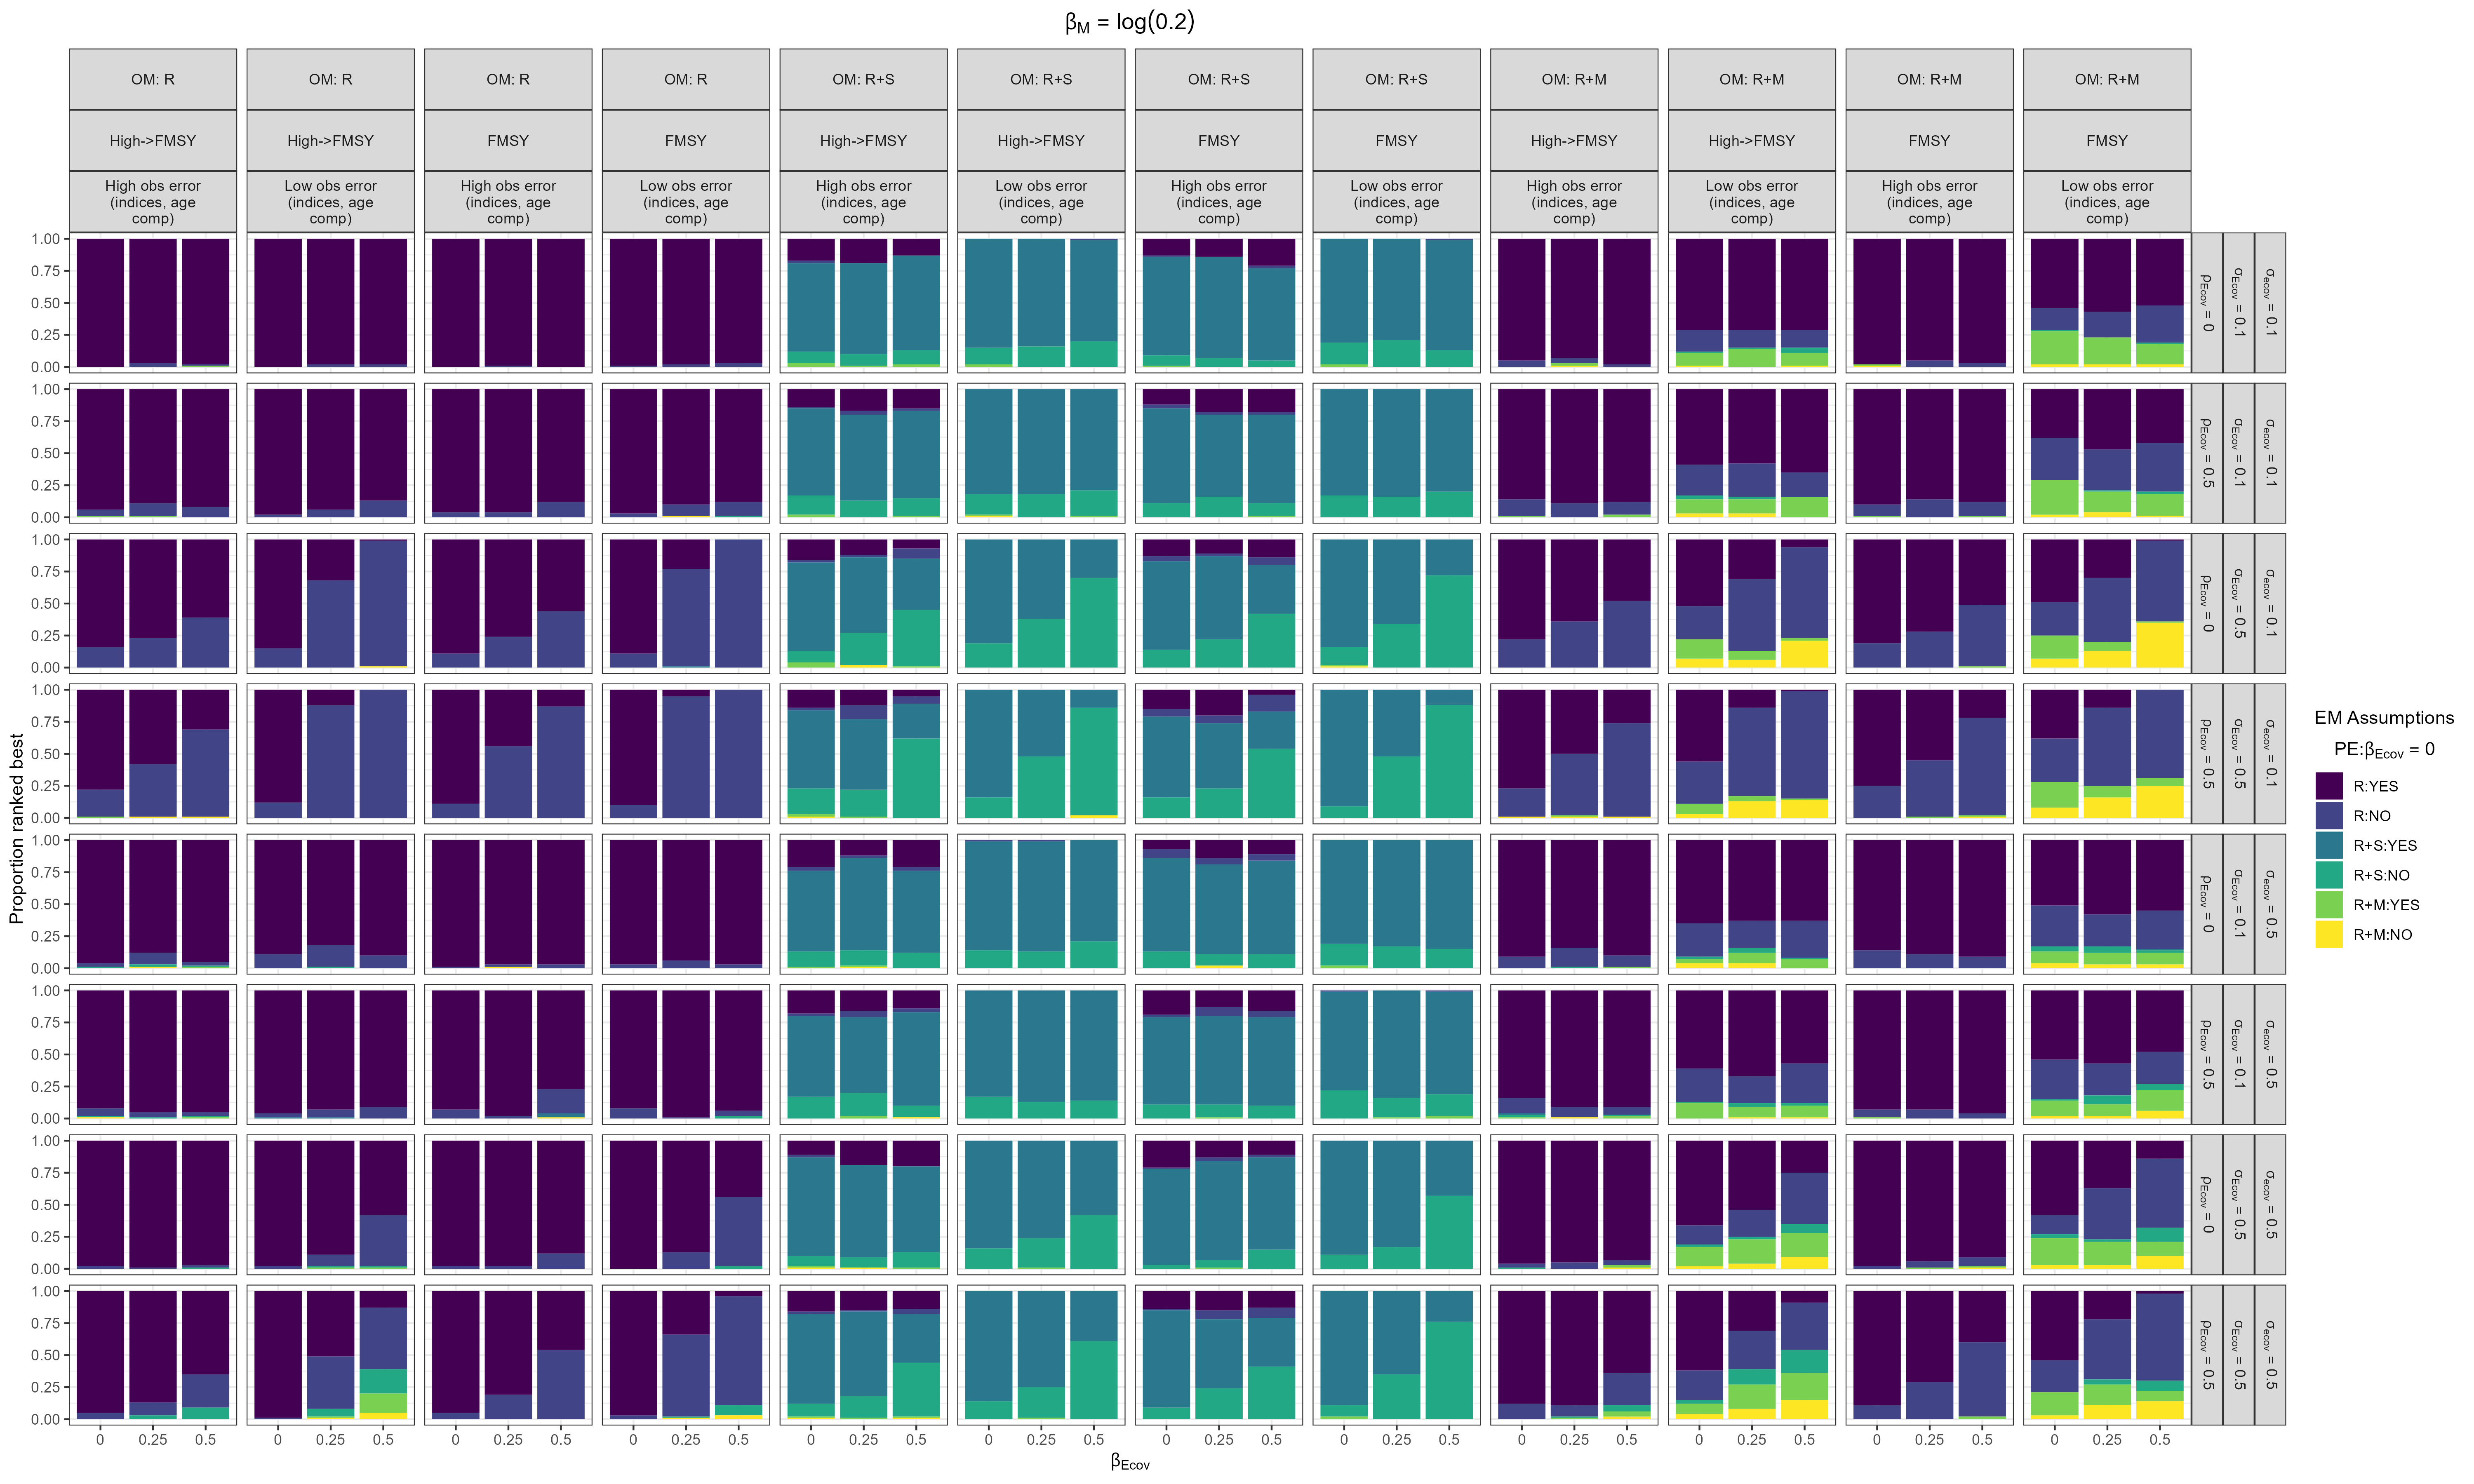
\includegraphics[height = \textheight]{proportion_best_AIC_M_fixed.png}
\end{center}
\end{figure}
\end{landscape}

\begin{landscape}
\begin{figure}
\caption{Proportion of simulated data sets for each operating model where the estimation model type (process error and covariate effect assumptions) had the lowest AIC. All estimating models assumed the mean mortality parameter $\beta_\text{M} = \log 0.2$.}\label{aic_rank_M_estimated}
\begin{center}
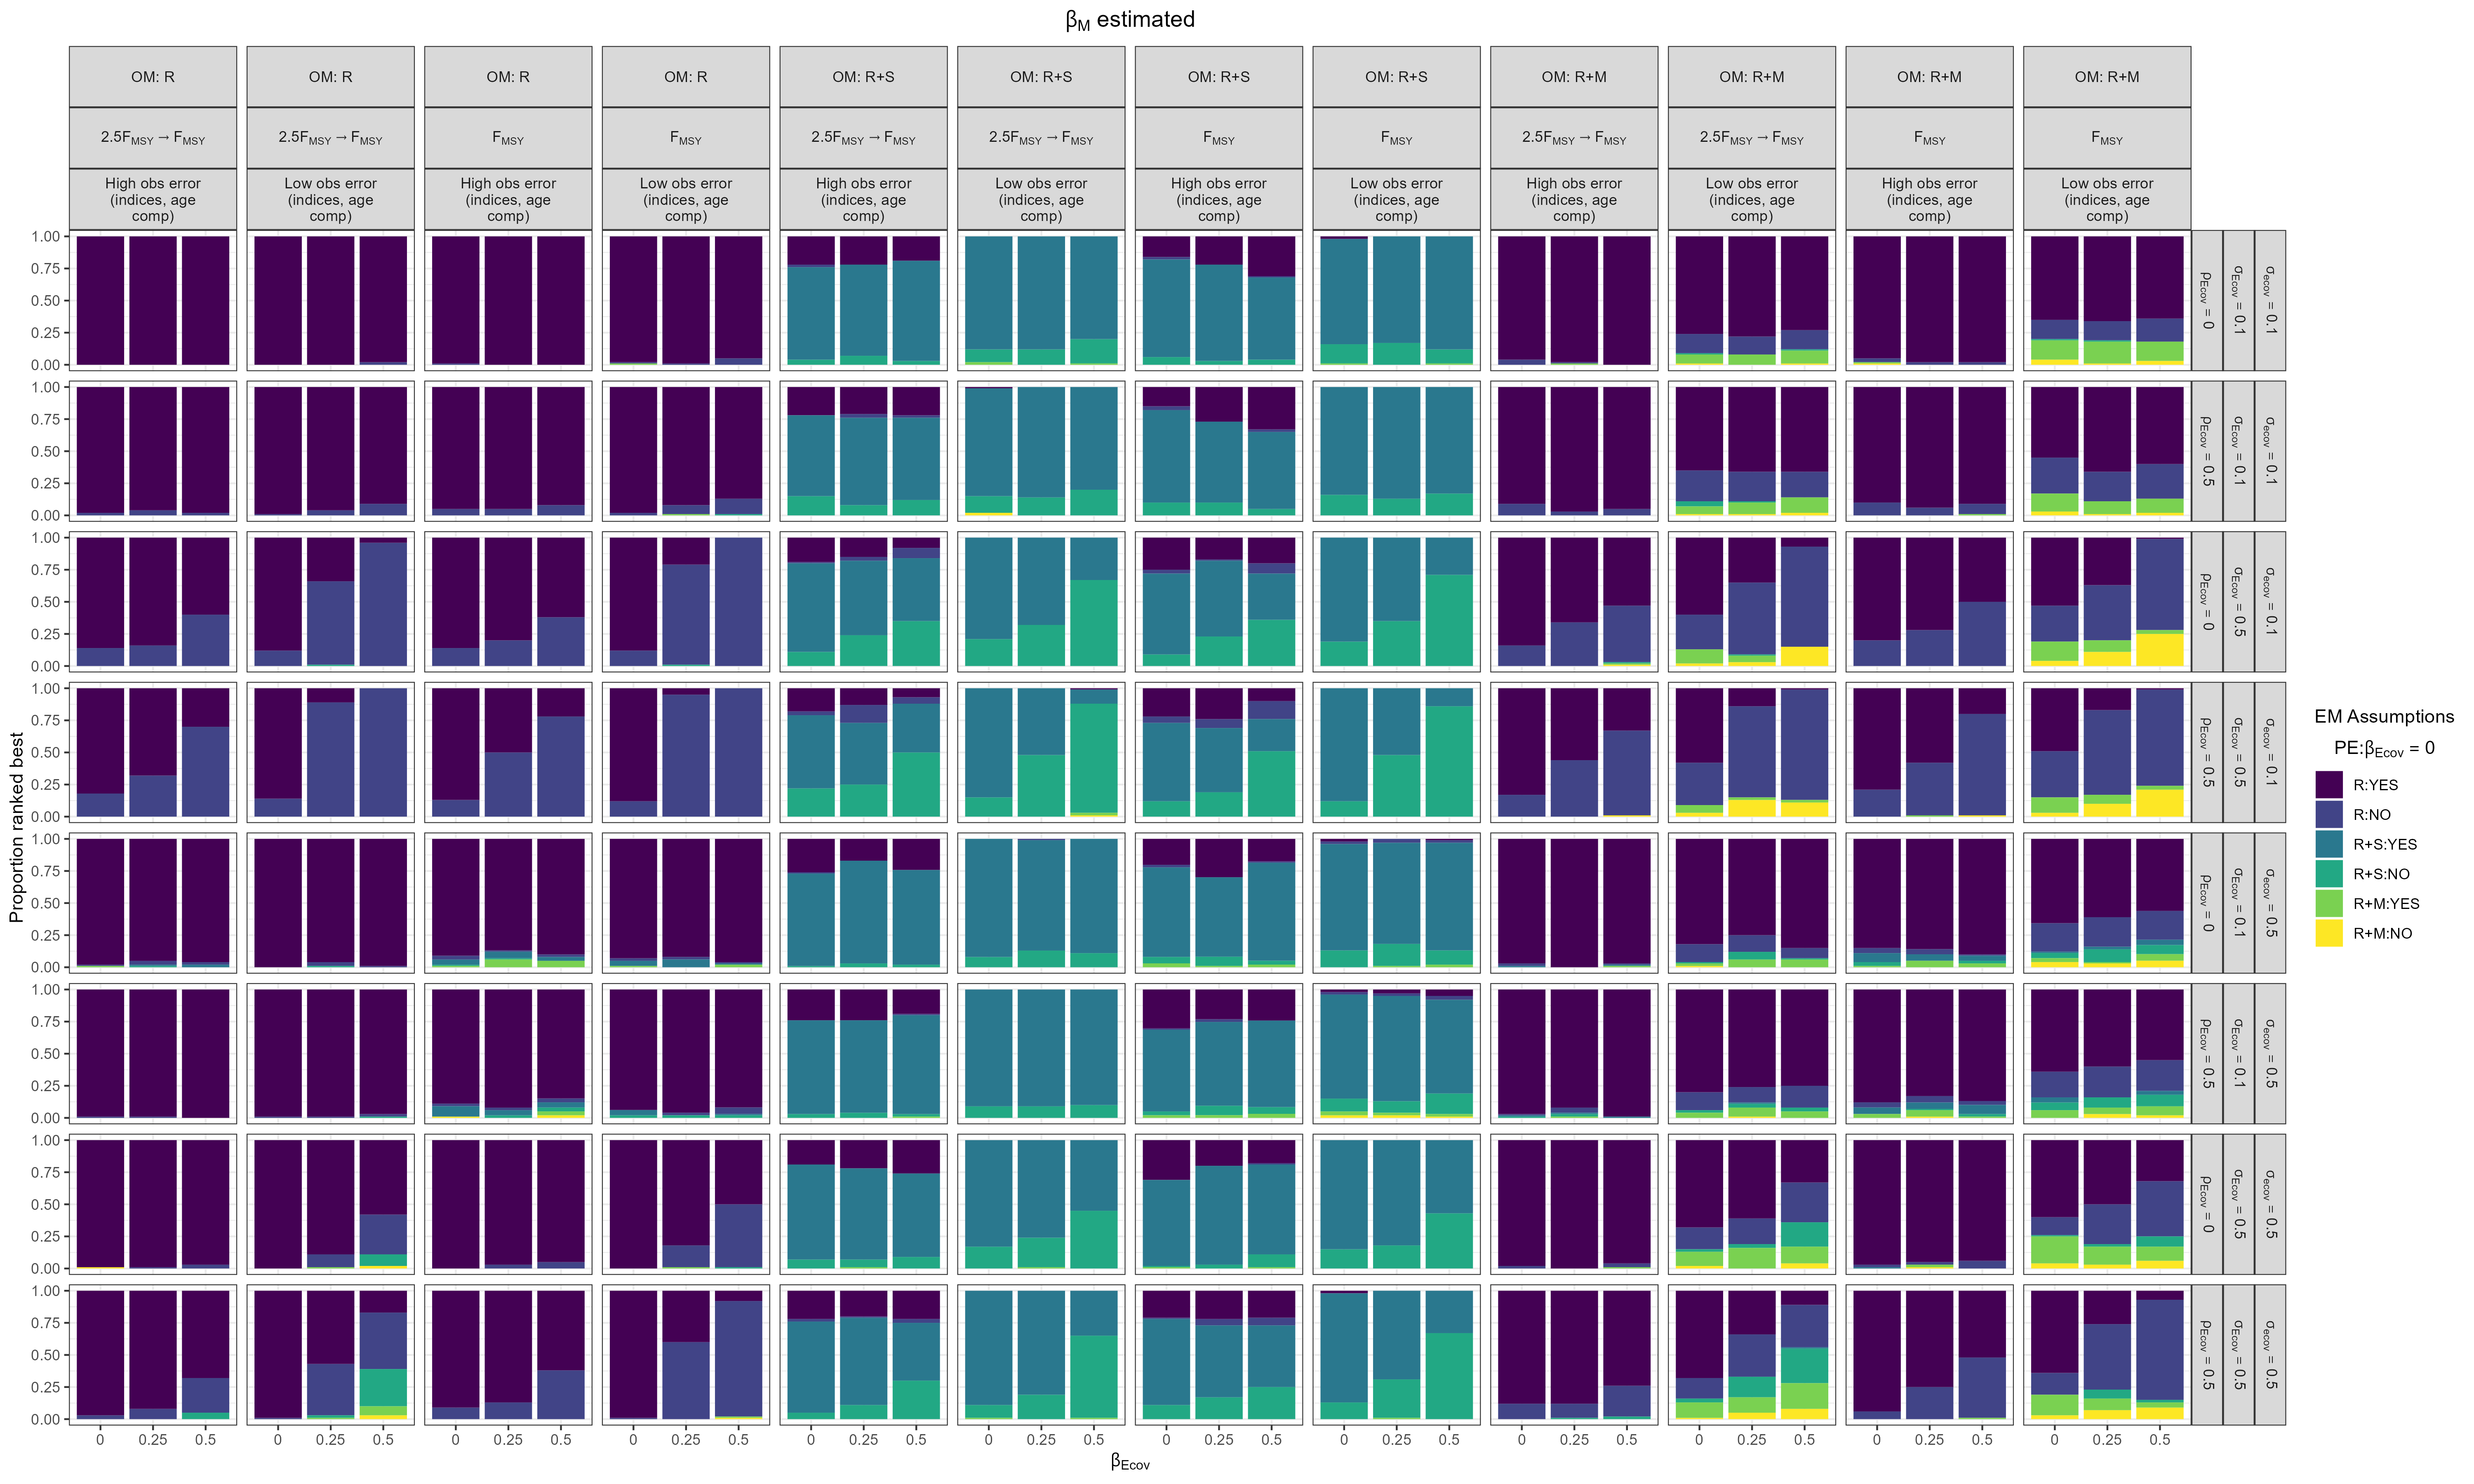
\includegraphics[height = \textheight]{proportion_best_AIC_M_estimated.png}
\end{center}
\end{figure}
\end{landscape}

\begin{landscape}
\begin{figure}
\caption{Median relative error of the estimated environmental effect on natural mortality $\beta_\text{Ecov}$ from fitting simulated observations from each operating model with alternative process error assumptions in the estimating model. All estimating models assumed the mean mortality parameter $\beta_\text{M} = \log 0.2$.}\label{Ecov_beta_bias_M_fixed}
\begin{center}
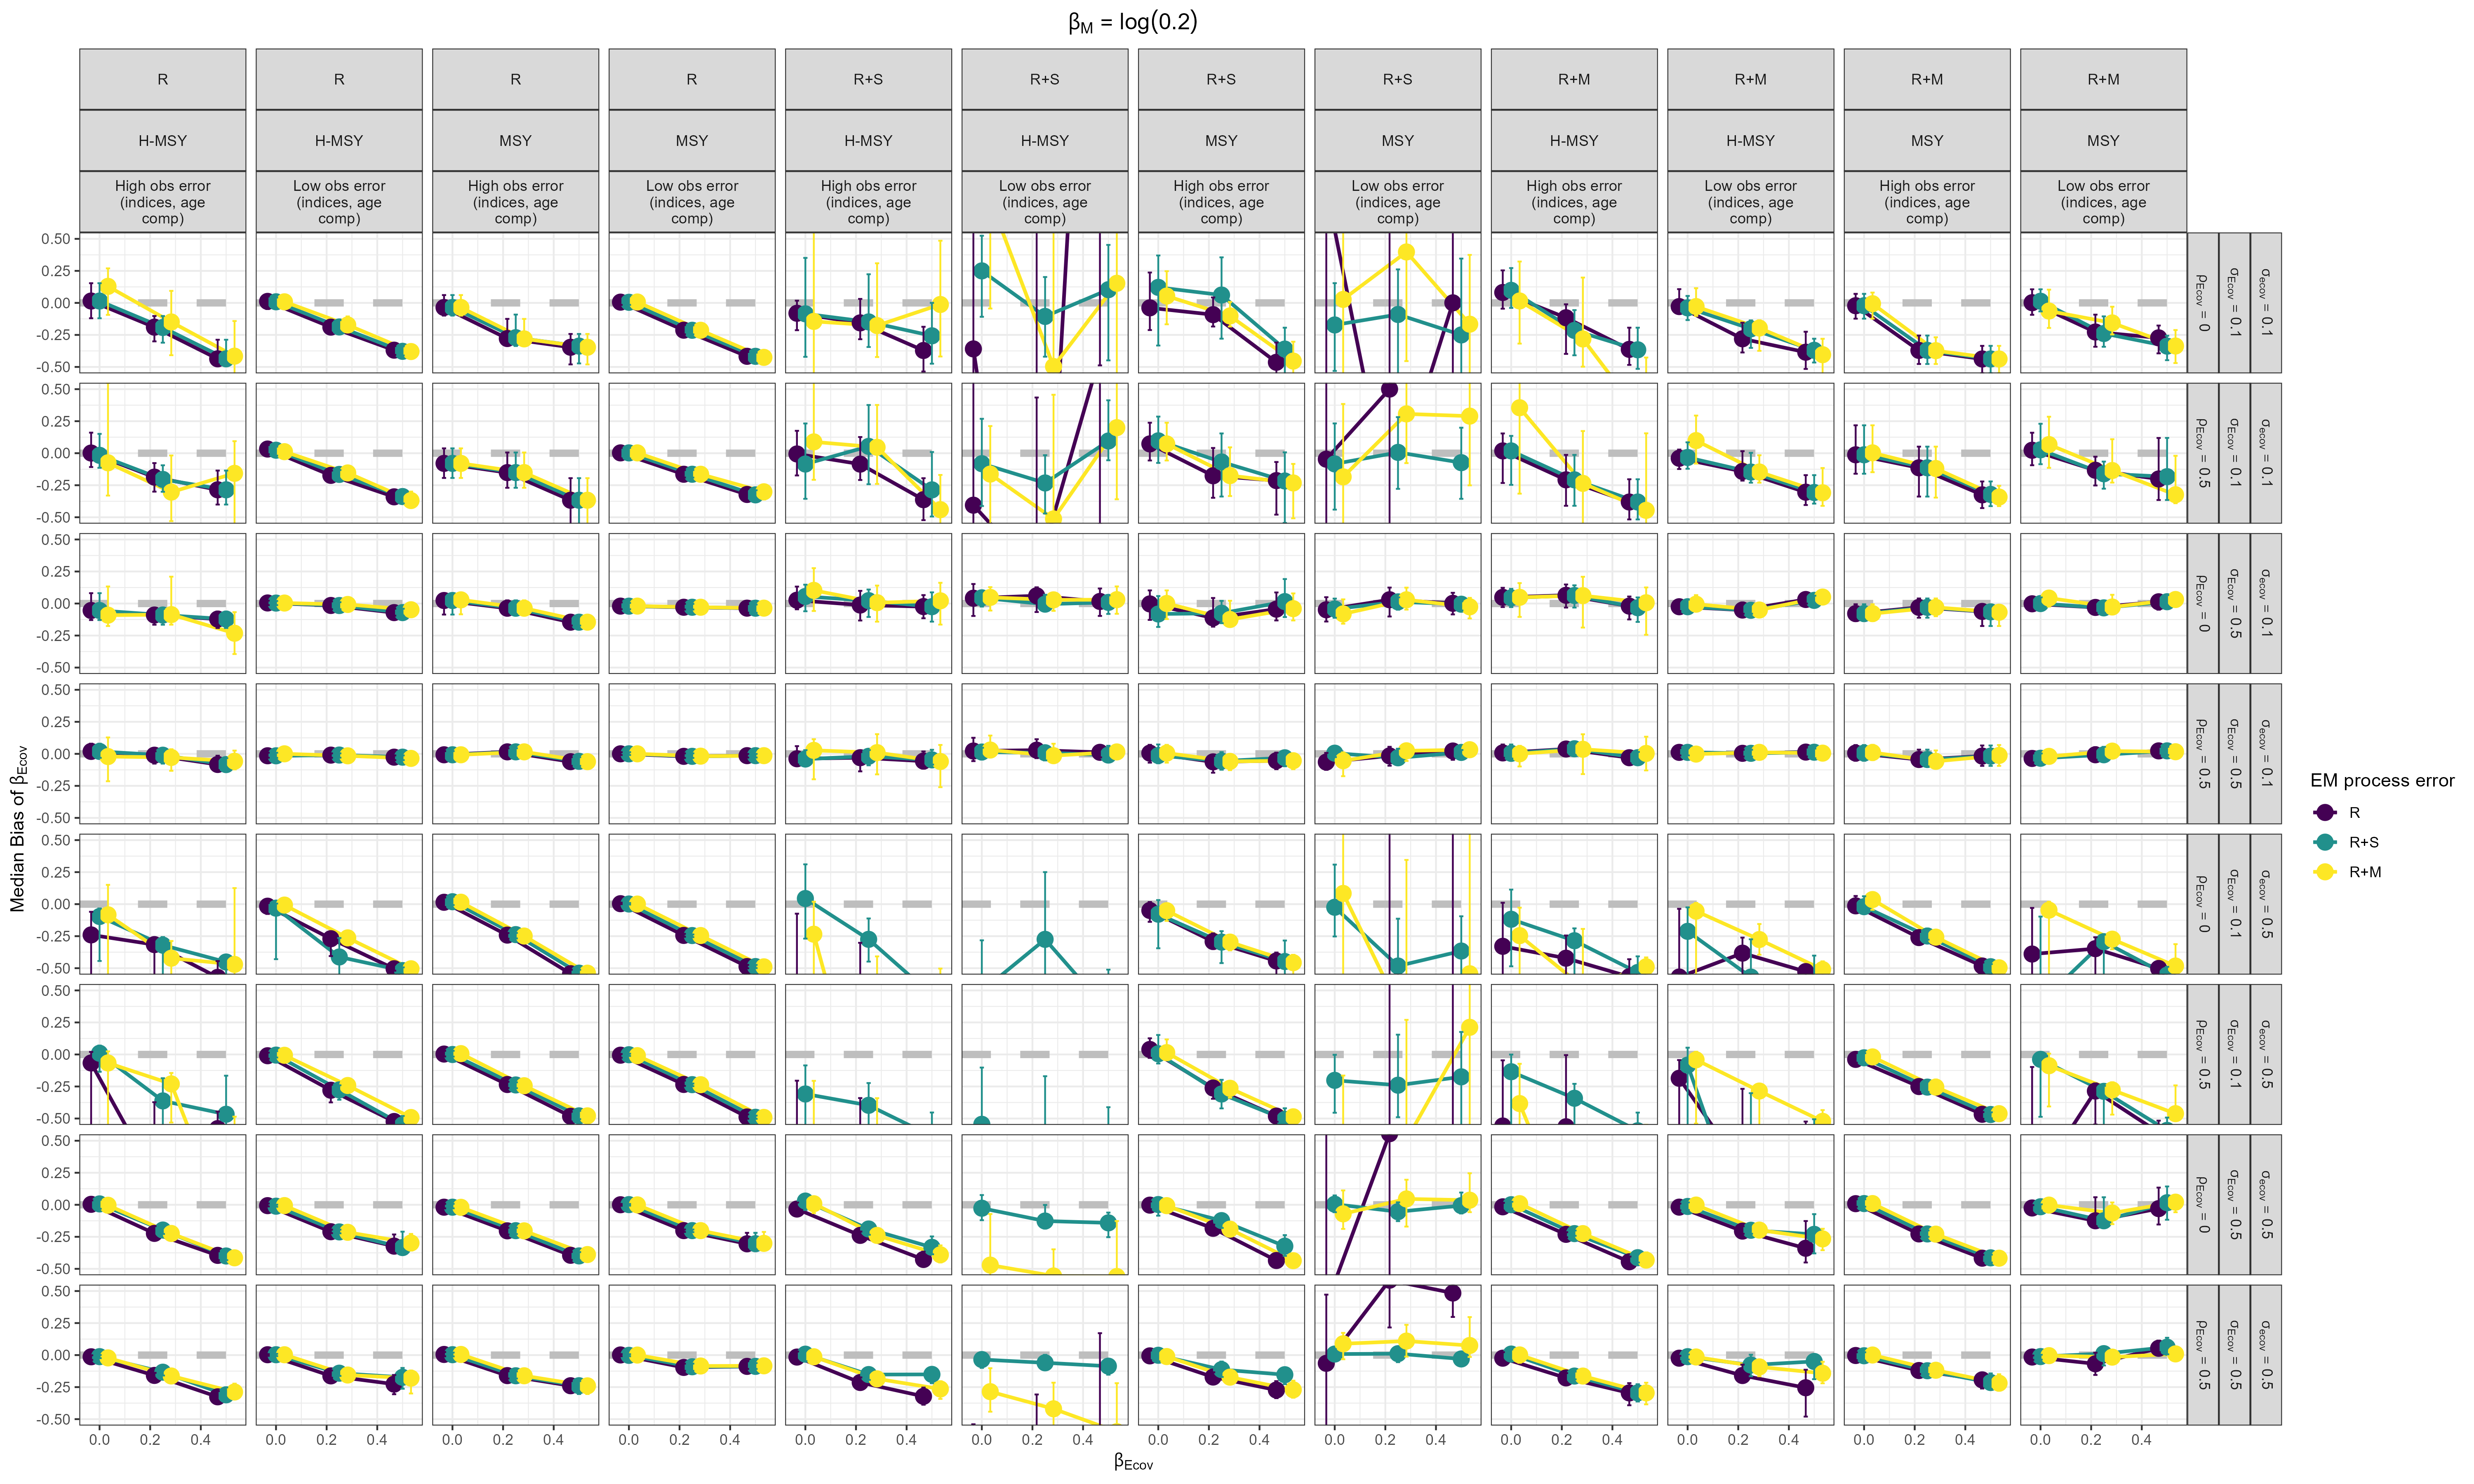
\includegraphics[height = \textheight]{Ecov_beta_bias_all_PE_effect_M_fixed.png}
\end{center}
\end{figure}
\end{landscape}

\begin{landscape}
\begin{figure}
\caption{Median relative error of the estimated environmental effect on natural mortality $\beta_\text{Ecov}$ from fitting simulated observations from each operating model with alternative process error assumptions in the estimating model. All estimating models assumed the mean mortality parameter $\beta_\text{M}$ is also estimated.}\label{Ecov_beta_bias_M_estimated}
\begin{center}
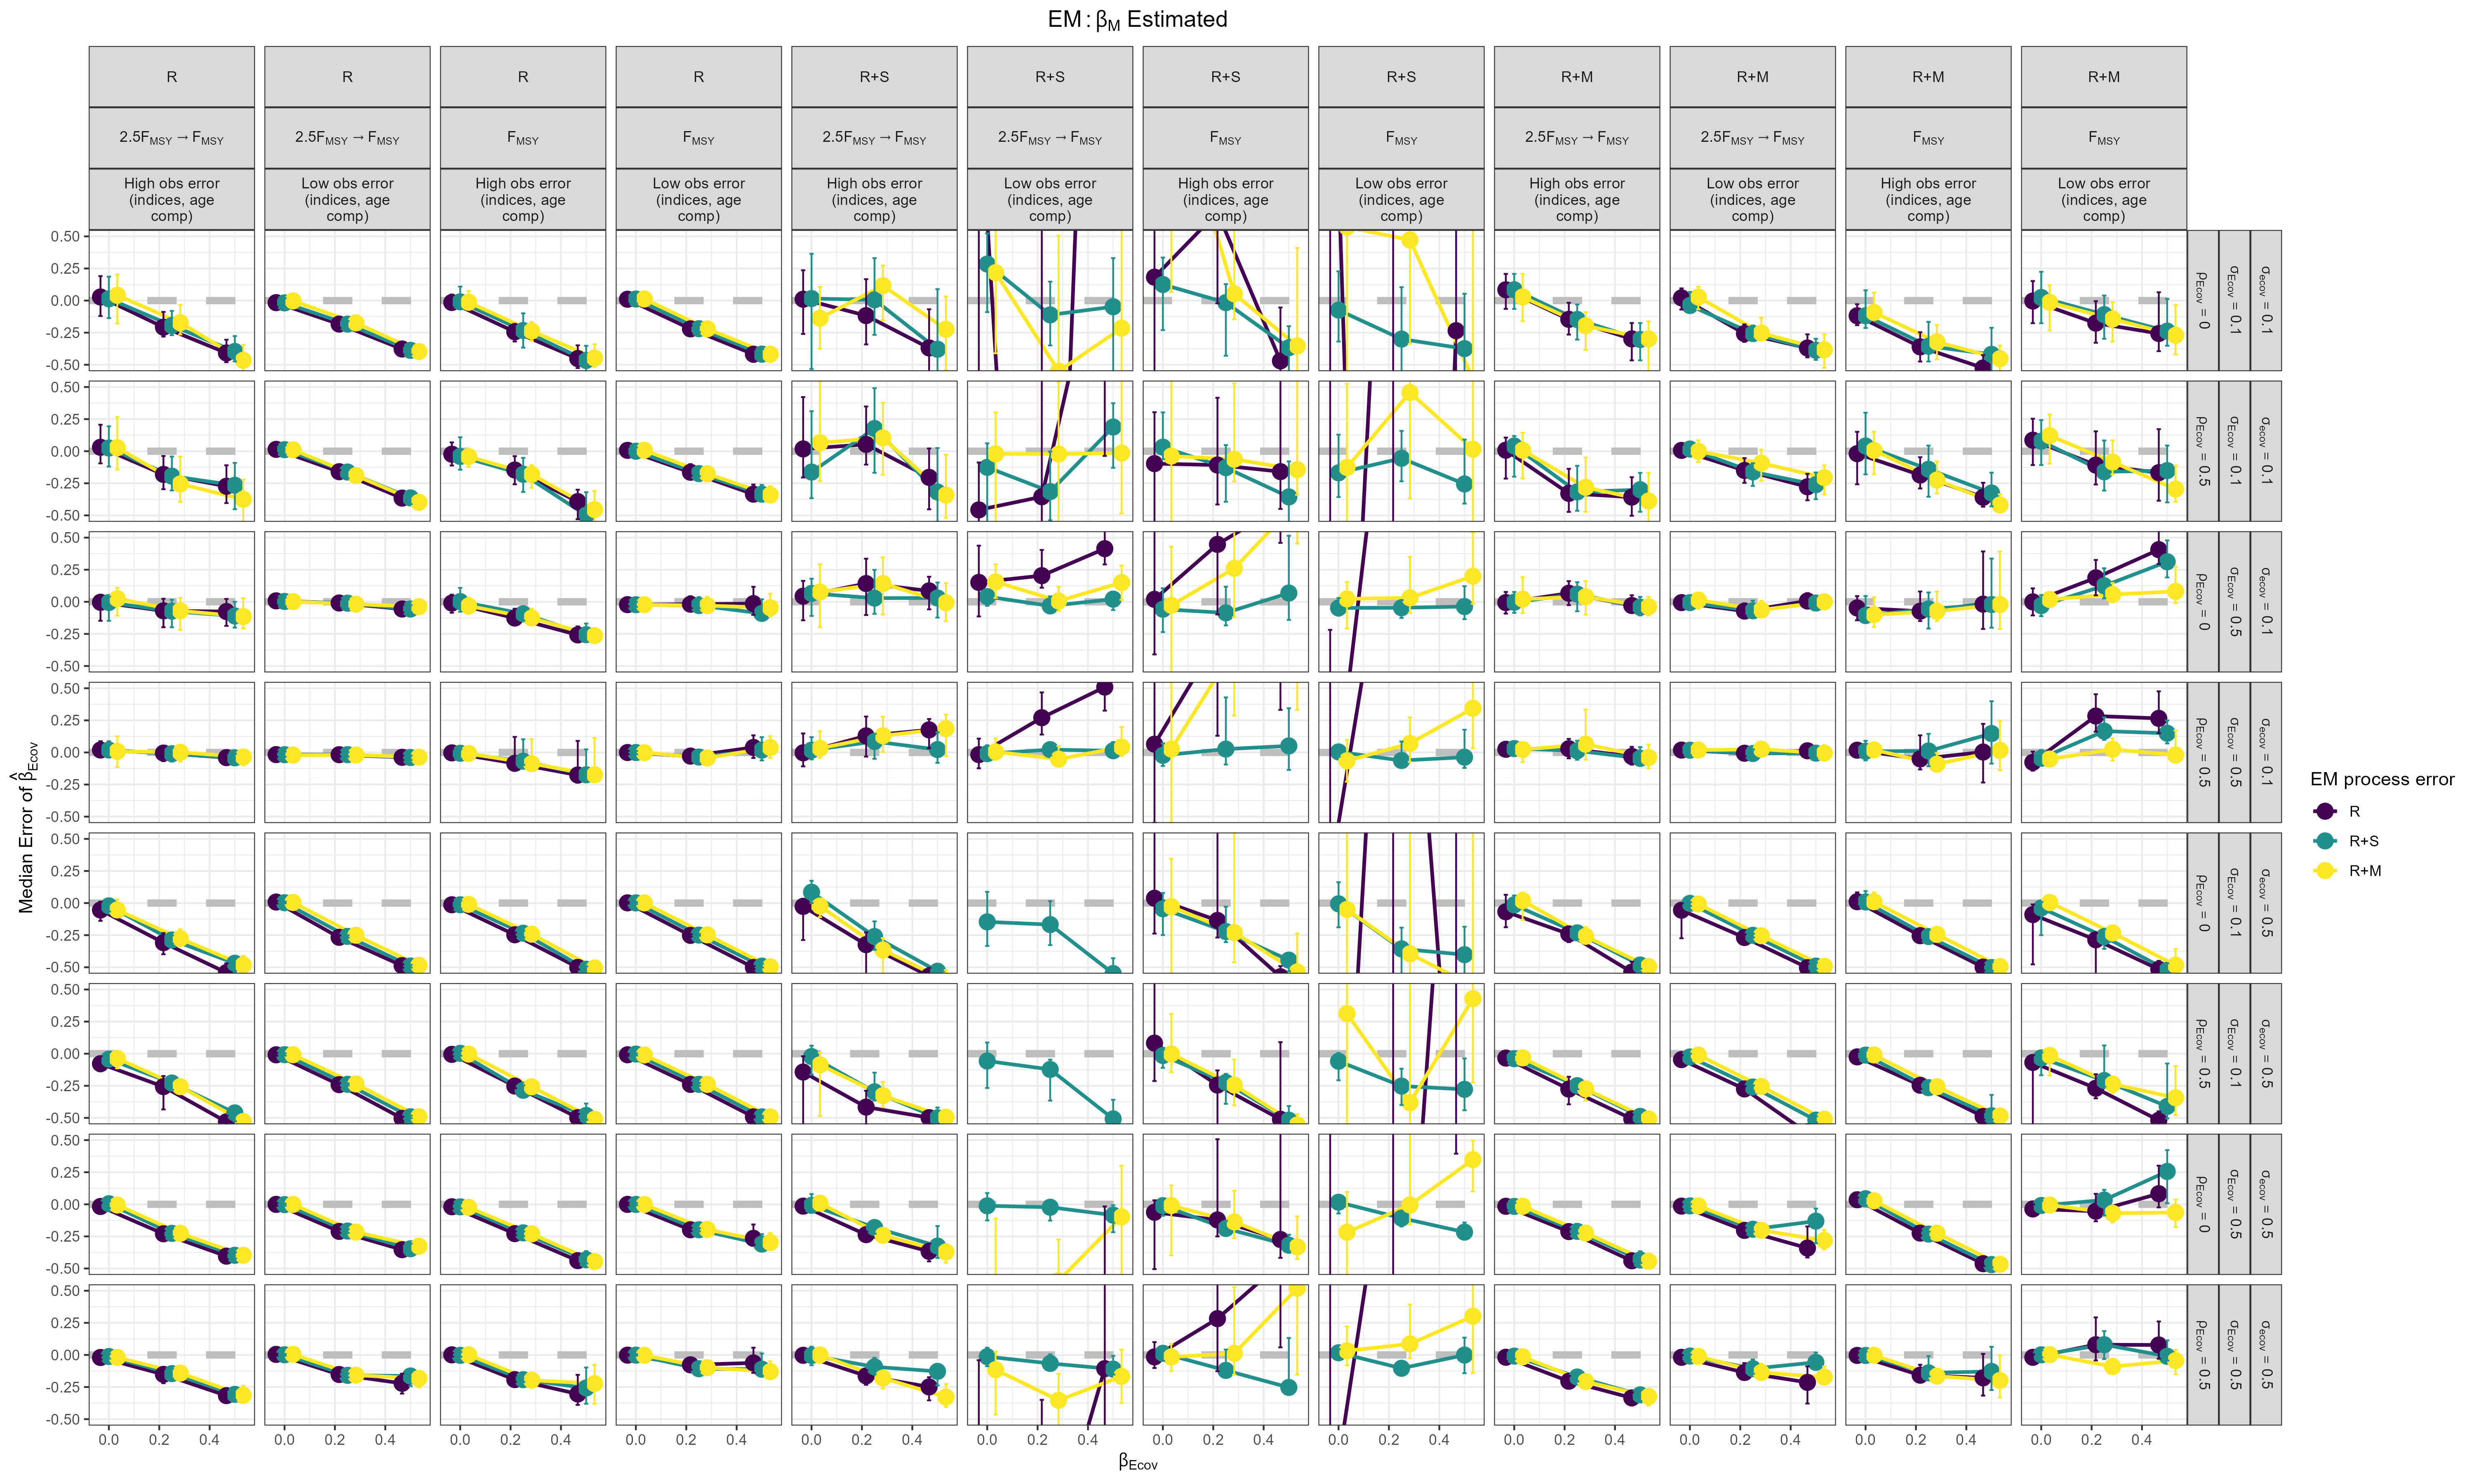
\includegraphics[height = \textheight]{Ecov_beta_bias_all_PE_effect_M_estimated.png}
\end{center}
\end{figure}
\end{landscape}

\begin{landscape}
\begin{figure}
\caption{Median relative error of the estimated mean natural mortality parameter $\beta_\text{M}$ from fitting simulated observations from each operating model with the estimating model assuming $\beta_\text{Ecov} = 0$ under alternative process error assumptions.}\label{mean_M_bias_Ecov_beta_fixed}
\begin{center}
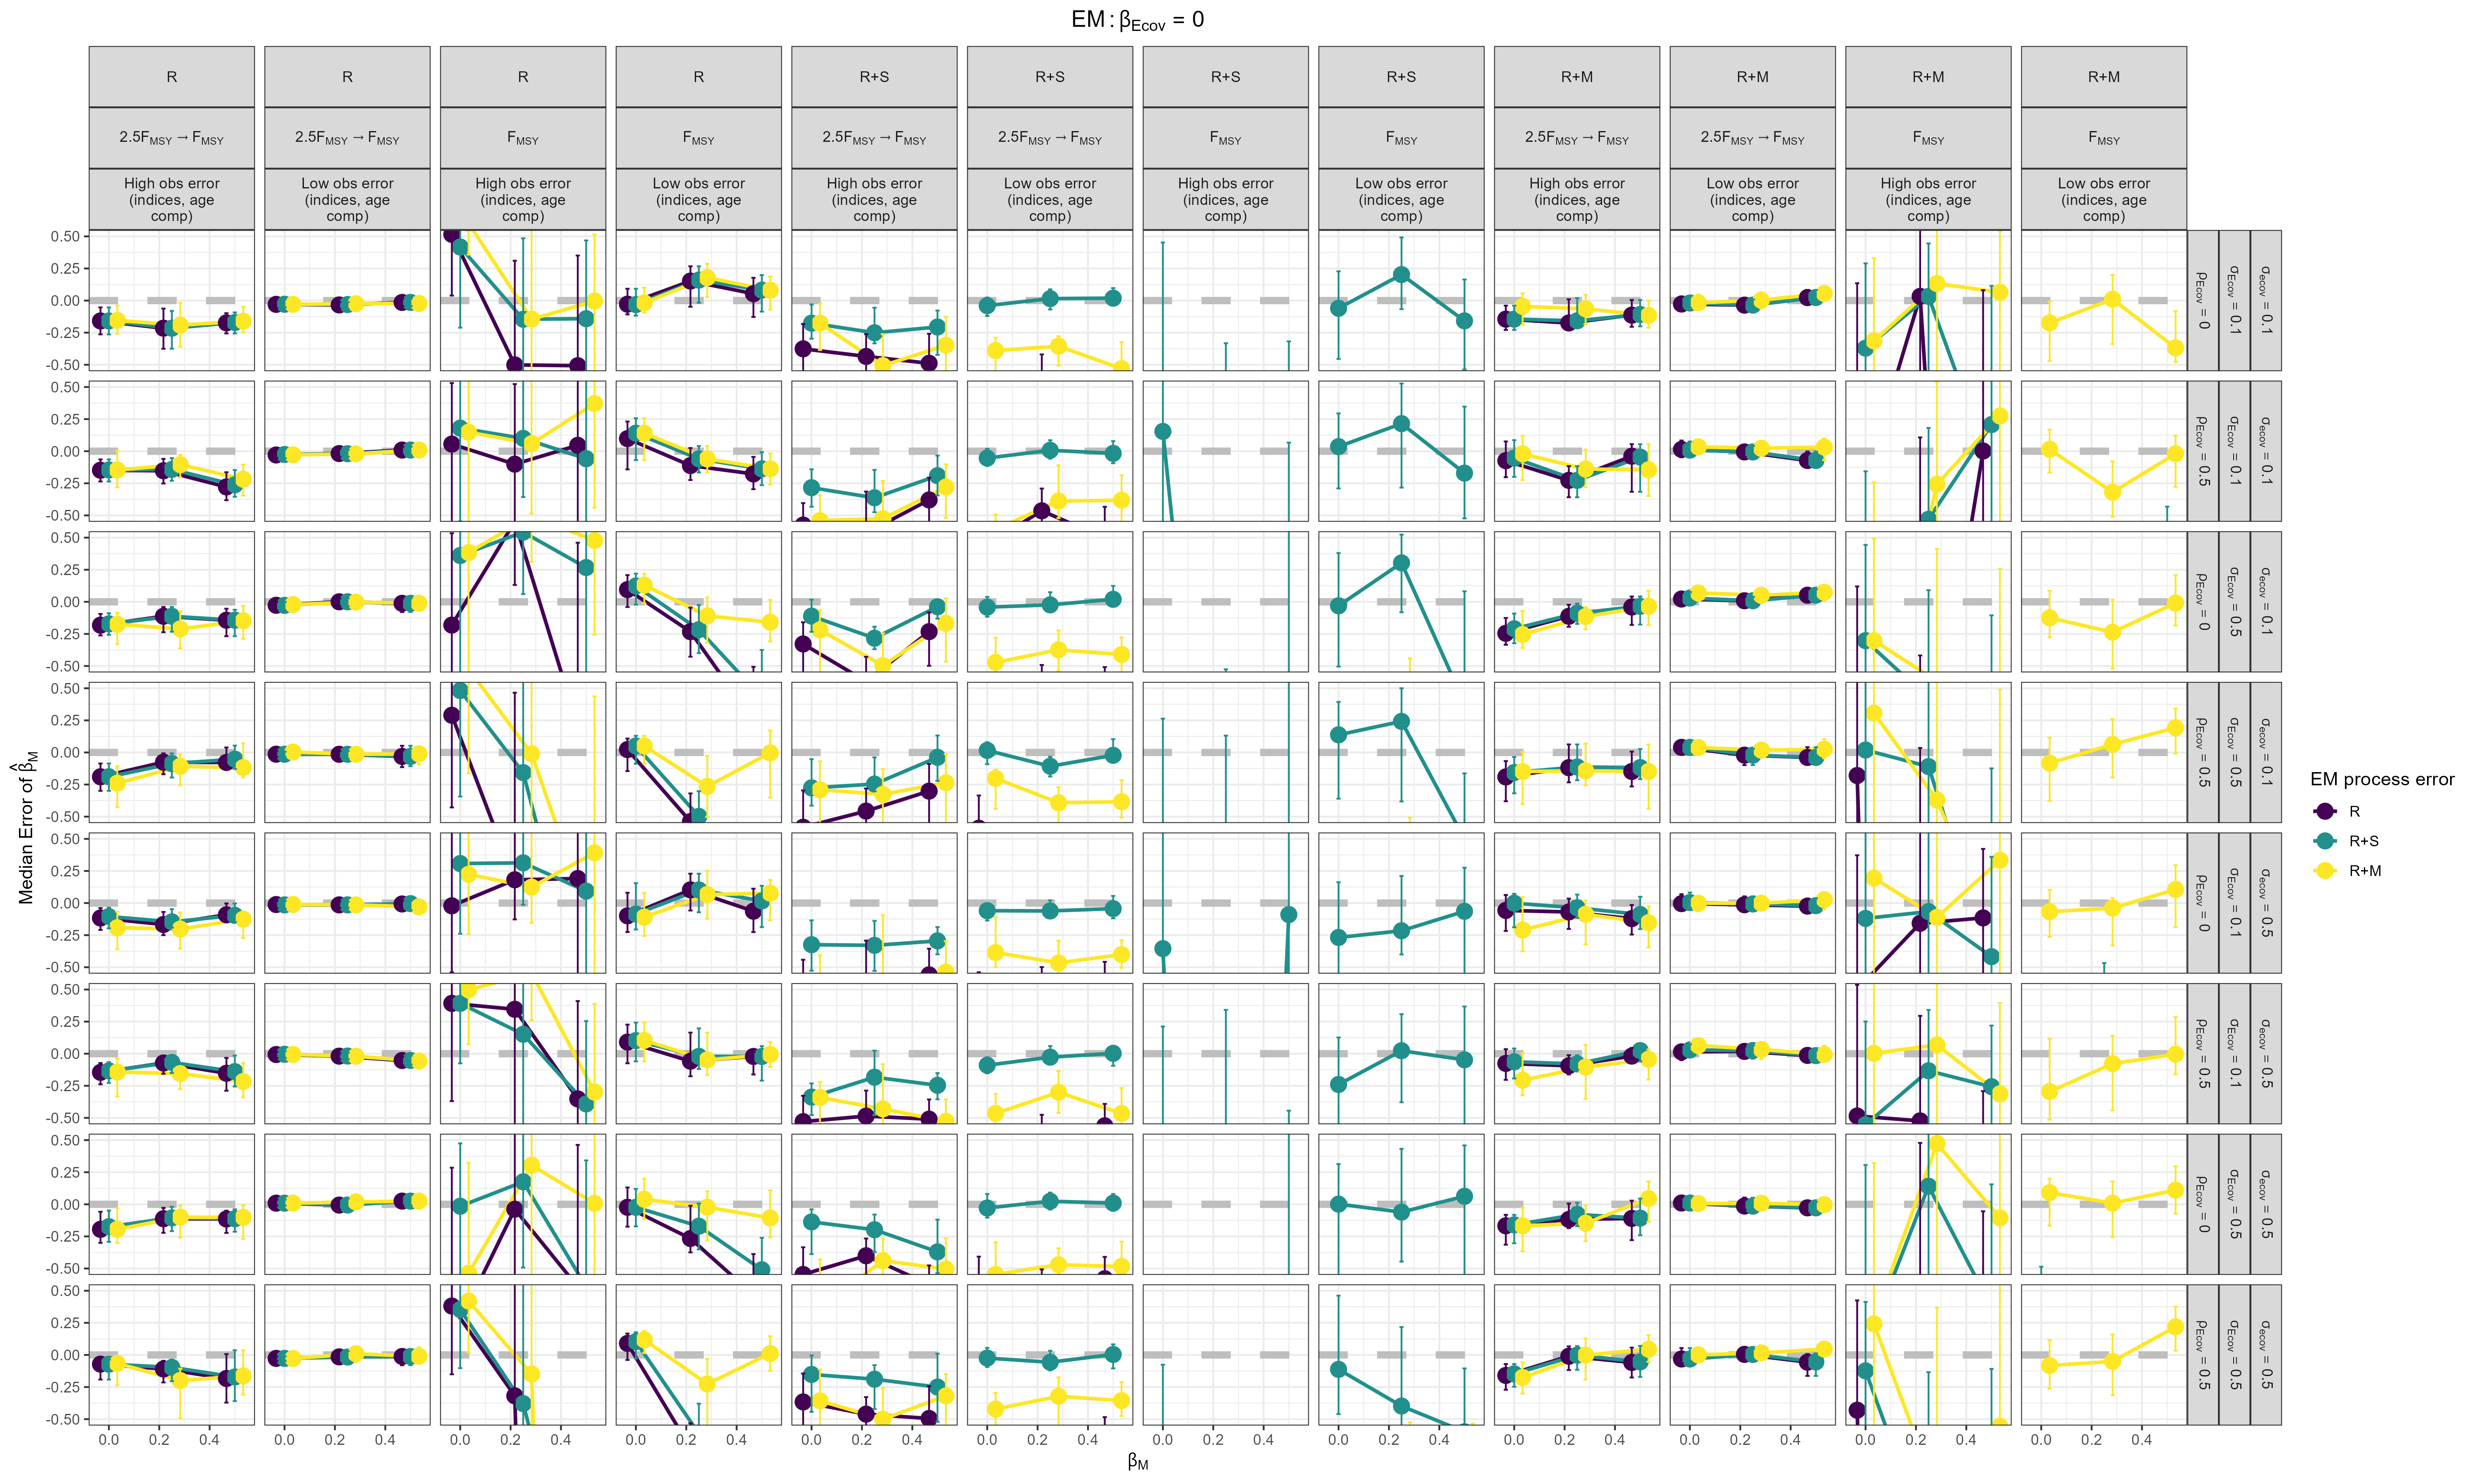
\includegraphics[height = \textheight]{mean_M_bias_all_PE_effect_Ecov_beta_fixed.png}
\end{center}
\end{figure}
\end{landscape}

\begin{landscape}
\begin{figure}
\caption{Median relative error of the estimated mean natural mortality parameter $\beta_\text{M}$ from fitting simulated observations from each operating model with the estimating model estimating $\beta_\text{Ecov} = 0$ under alternative process error assumptions.}\label{mean_M_bias_Ecov_beta_estimated}
\begin{center}
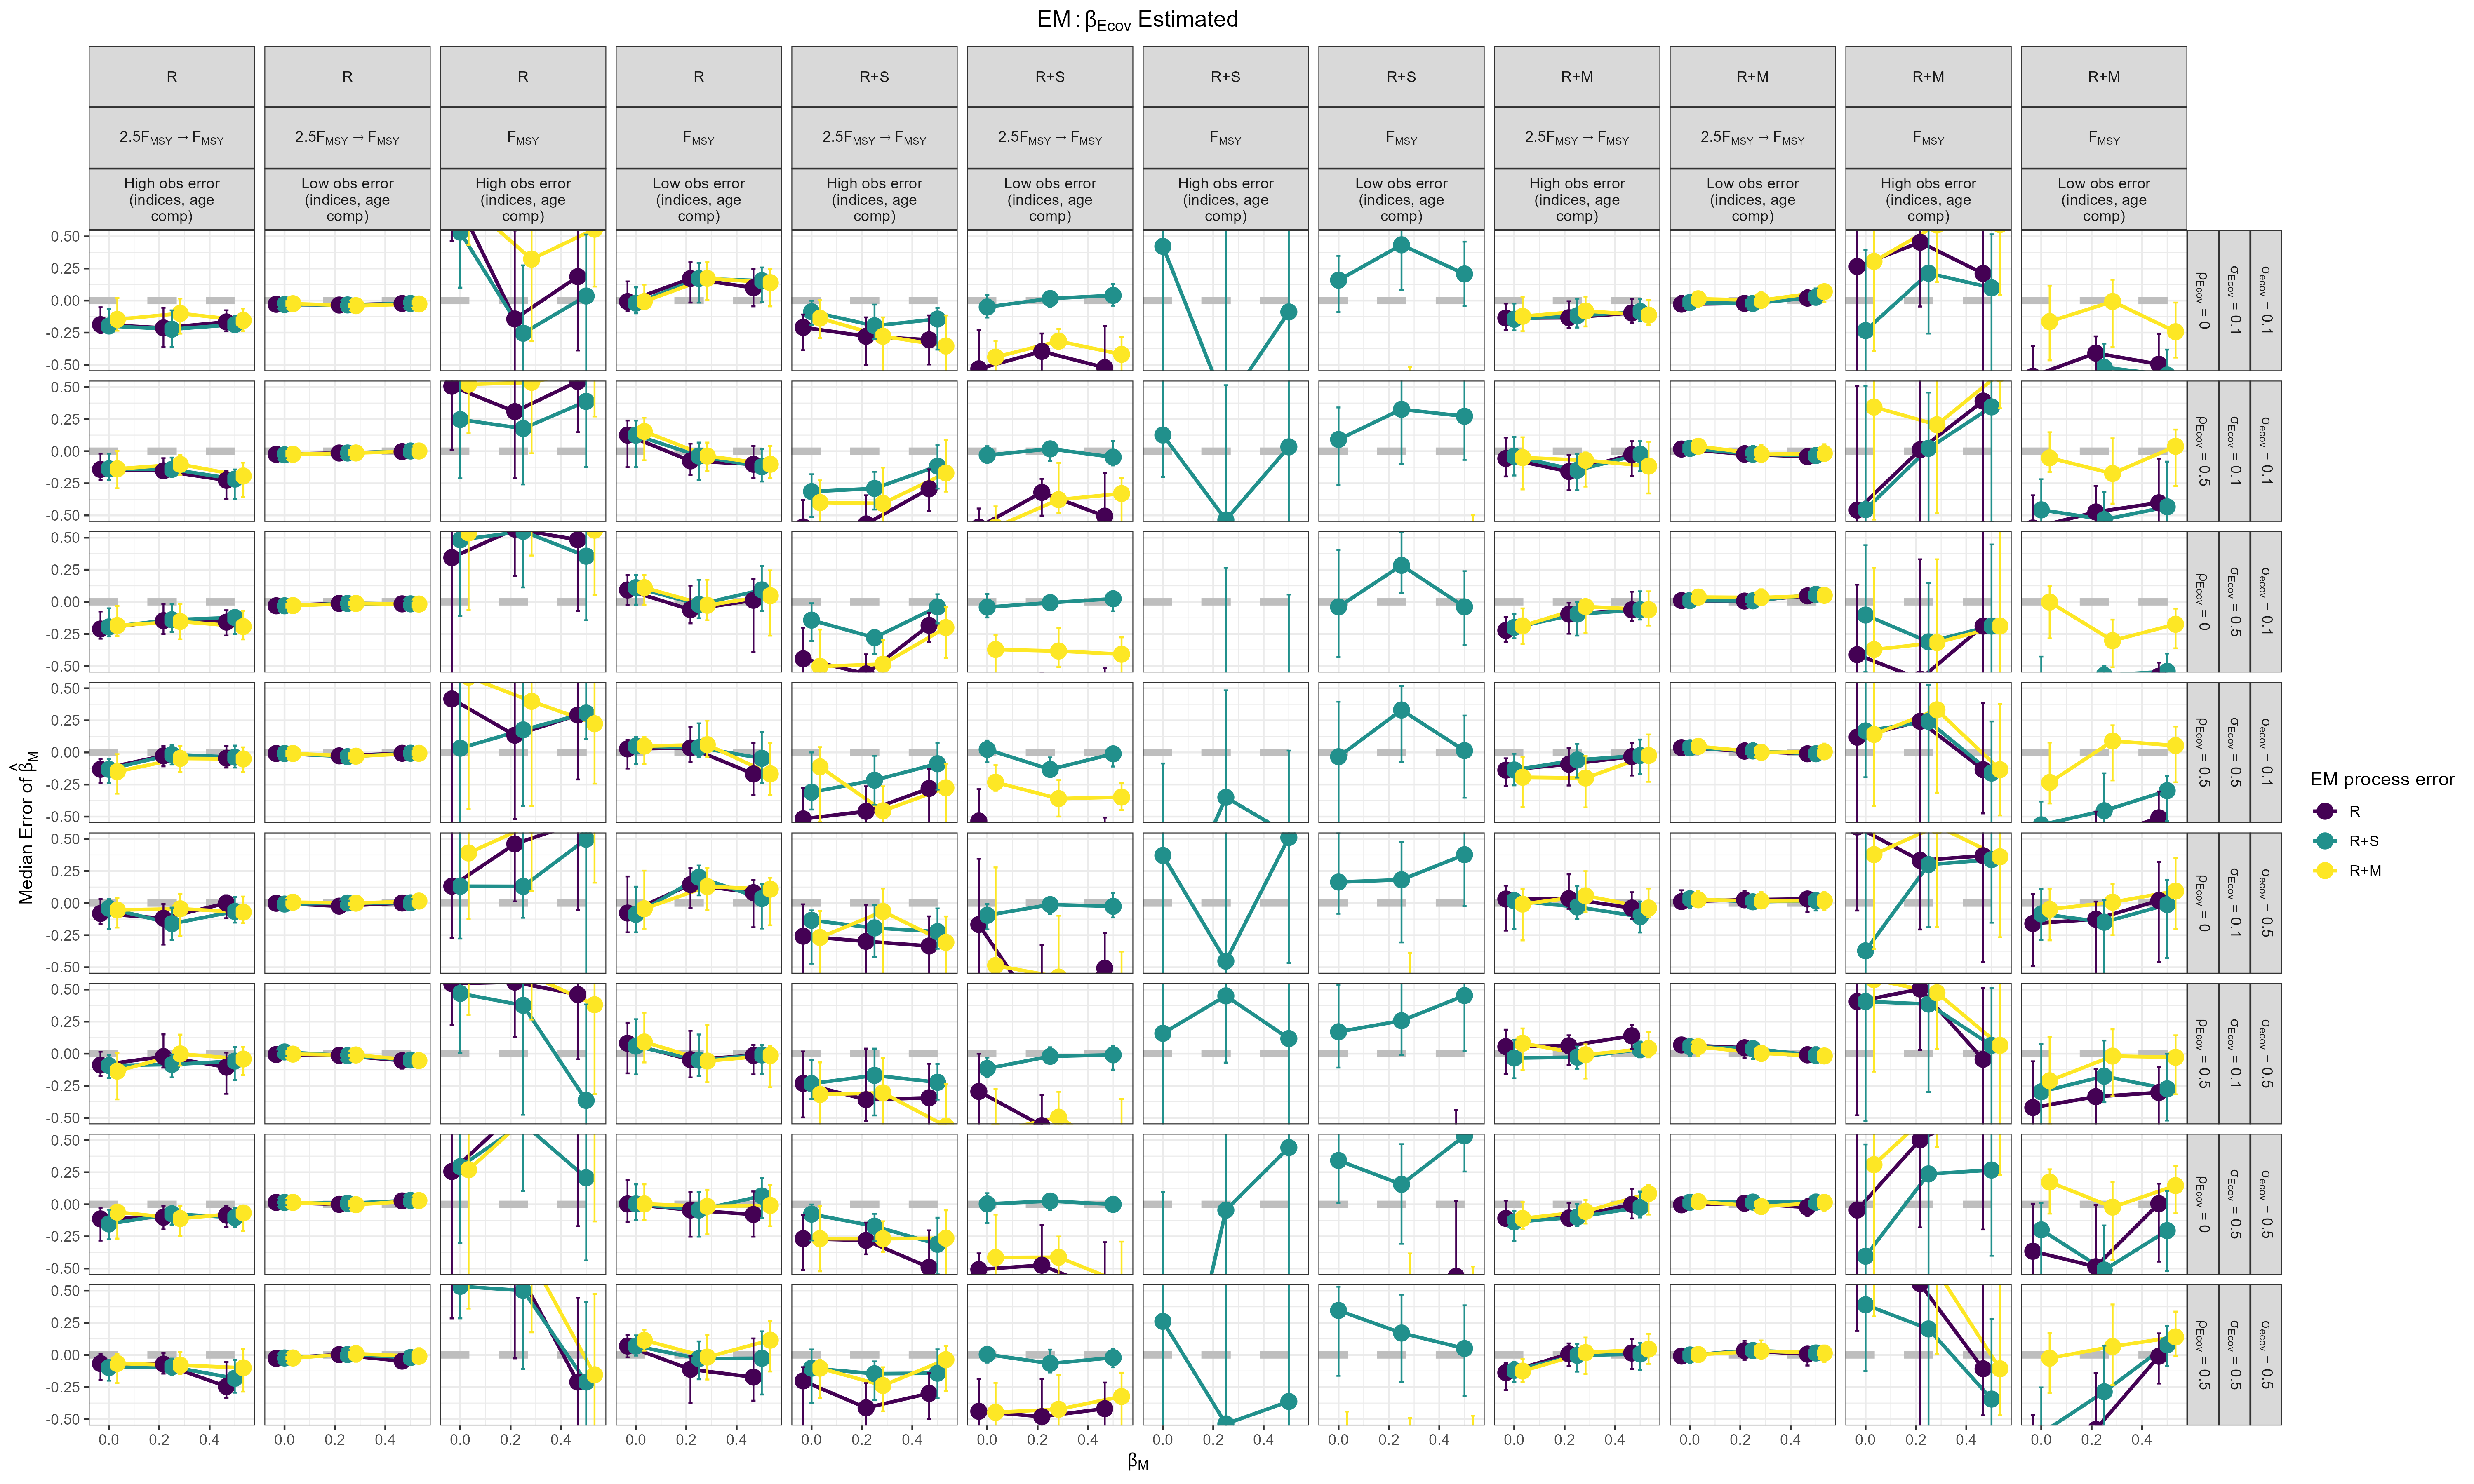
\includegraphics[height = \textheight]{mean_M_bias_all_PE_effect_Ecov_beta_estimated.png}
\end{center}
\end{figure}
\end{landscape}

\begin{landscape}
\begin{figure}
\caption{Median relative error of annual natural mortality rate in years 1 (Start), 21 (Middle), and 40 (End) from fitting simulated observations from each operating model with alternative process error assumptions in the estimating model. Estimating models also assume the mean natural mortality parameter $\beta_\text{M} = \log 0.2$ and no environmental covariate effect $\beta_\text{Ecov} = 0$.}\label{annual_M_bias_M_fixed_beta_fixed}
\begin{center}
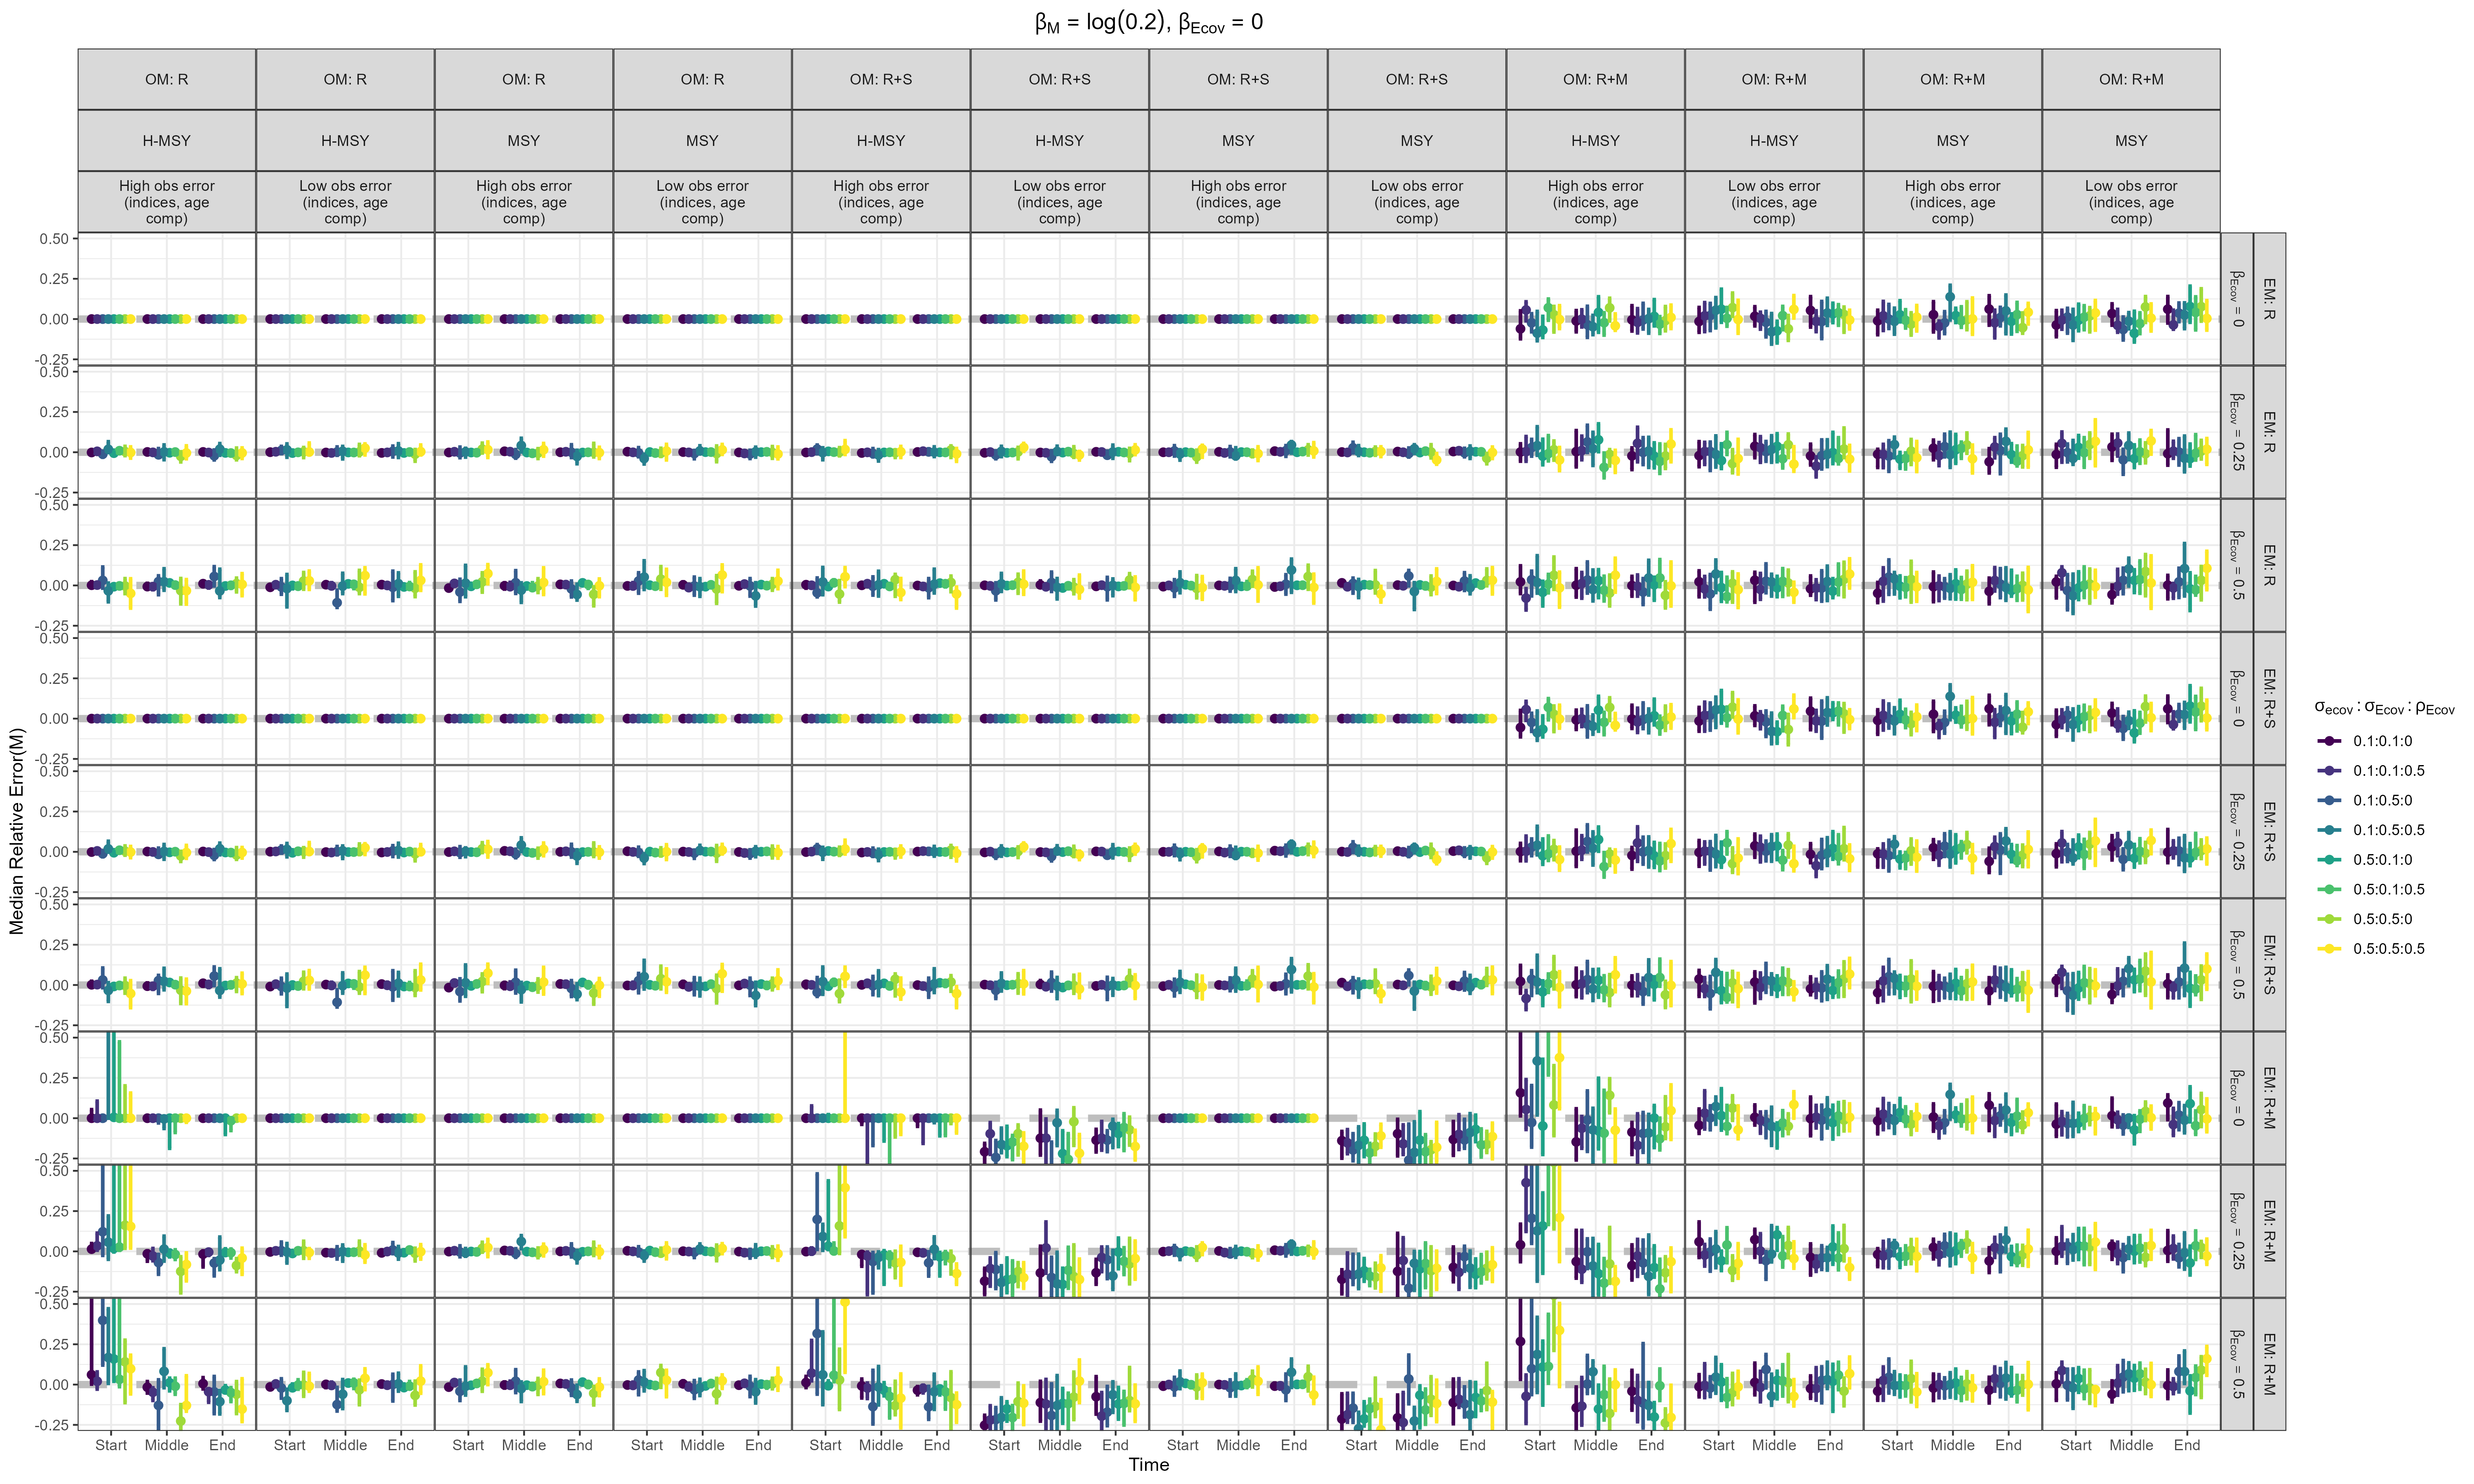
\includegraphics[height = \textheight]{annual_M_bias_all_PE_effect_M_fixed_beta_fixed.png}
\end{center}
\end{figure}
\end{landscape}

\begin{landscape}
\begin{figure}
\caption{Median relative error of annual natural mortality rate in years 1 (Start), 21 (Middle), and 40 (End) from fitting simulated observations from each operating model with alternative process error assumptions in the estimating model. Estimating models also assume the mean natural mortality parameter $\beta_\text{M} = \log 0.2$ and the environmental covariate effect $\beta_\text{Ecov}$ is estimated.}\label{annual_M_bias_M_fixed_beta_estimated}
\begin{center}
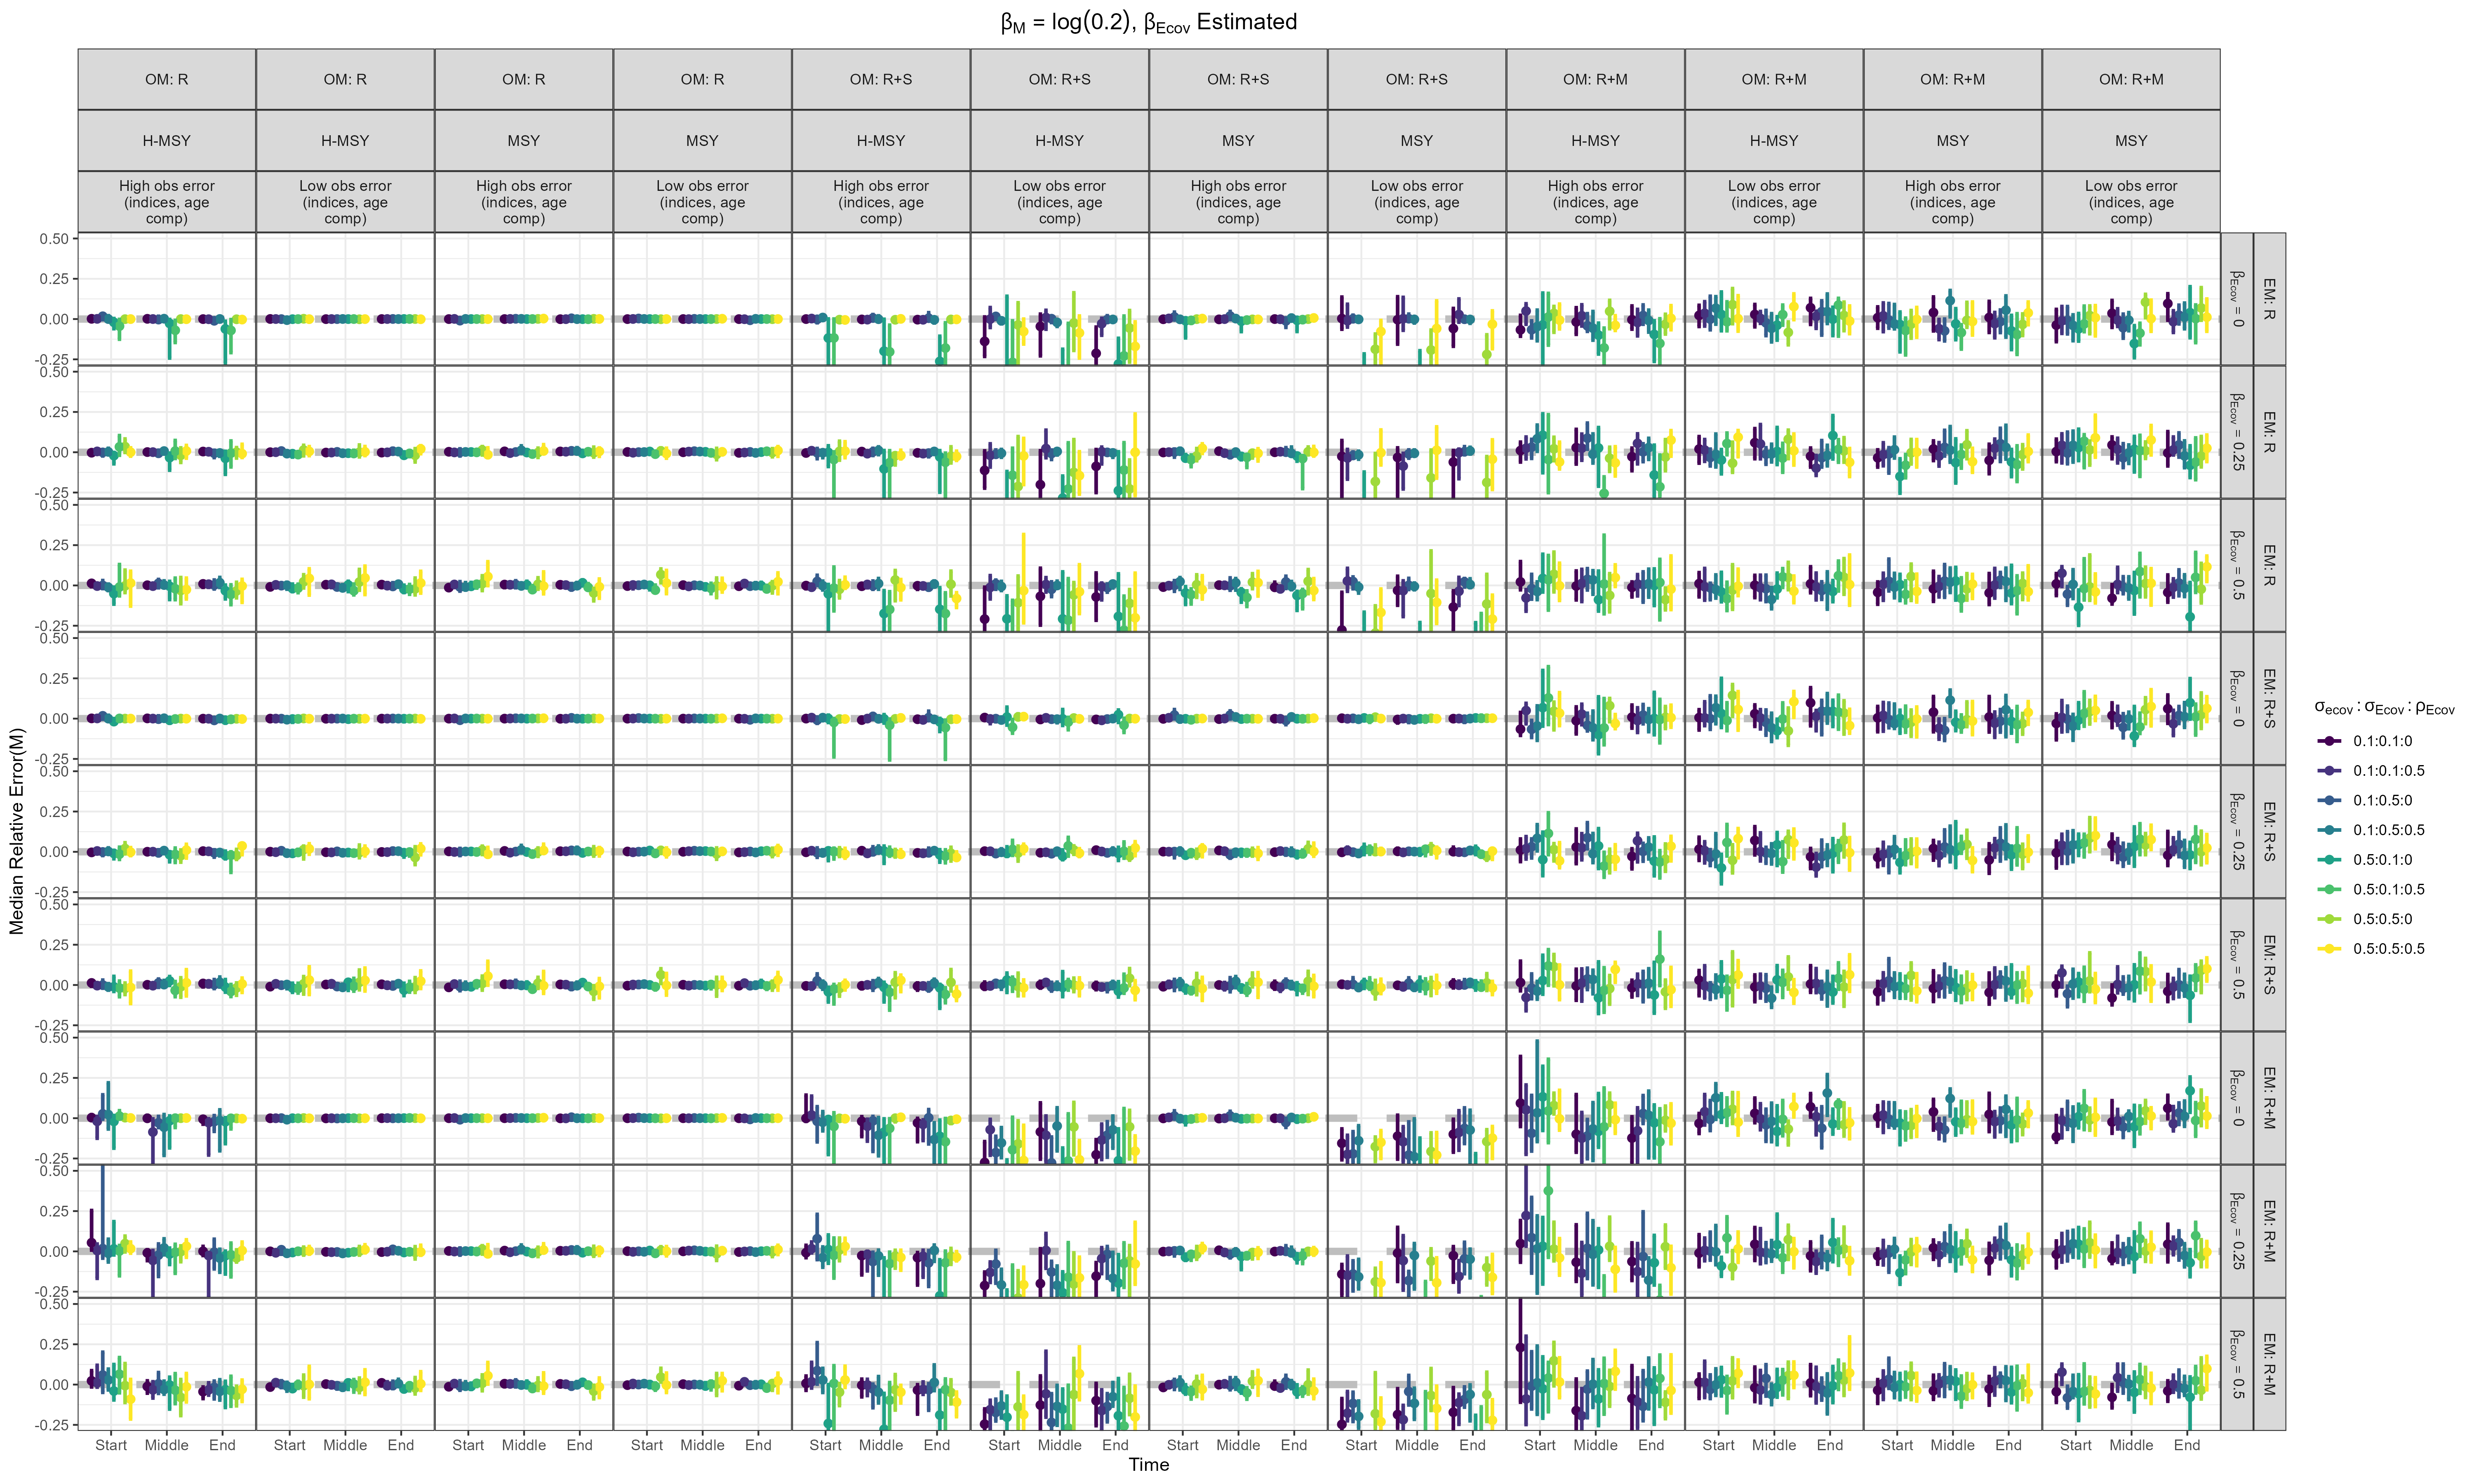
\includegraphics[height = \textheight]{annual_M_bias_all_PE_effect_M_fixed_beta_estimated.png}
\end{center}
\end{figure}
\end{landscape}

\begin{landscape}
\begin{figure}
\caption{Median relative error of annual natural mortality rate in years 1 (Start), 21 (Middle), and 40 (End) from fitting simulated observations from each operating model with alternative process error assumptions in the estimating model. Estimating models also assume both the mean natural mortality parameter $\beta_\text{M}$ and the environmental covariate effect $\beta_\text{Ecov}$ are estimated.}\label{annual_M_bias_M_estimated_beta_estimated}
\begin{center}
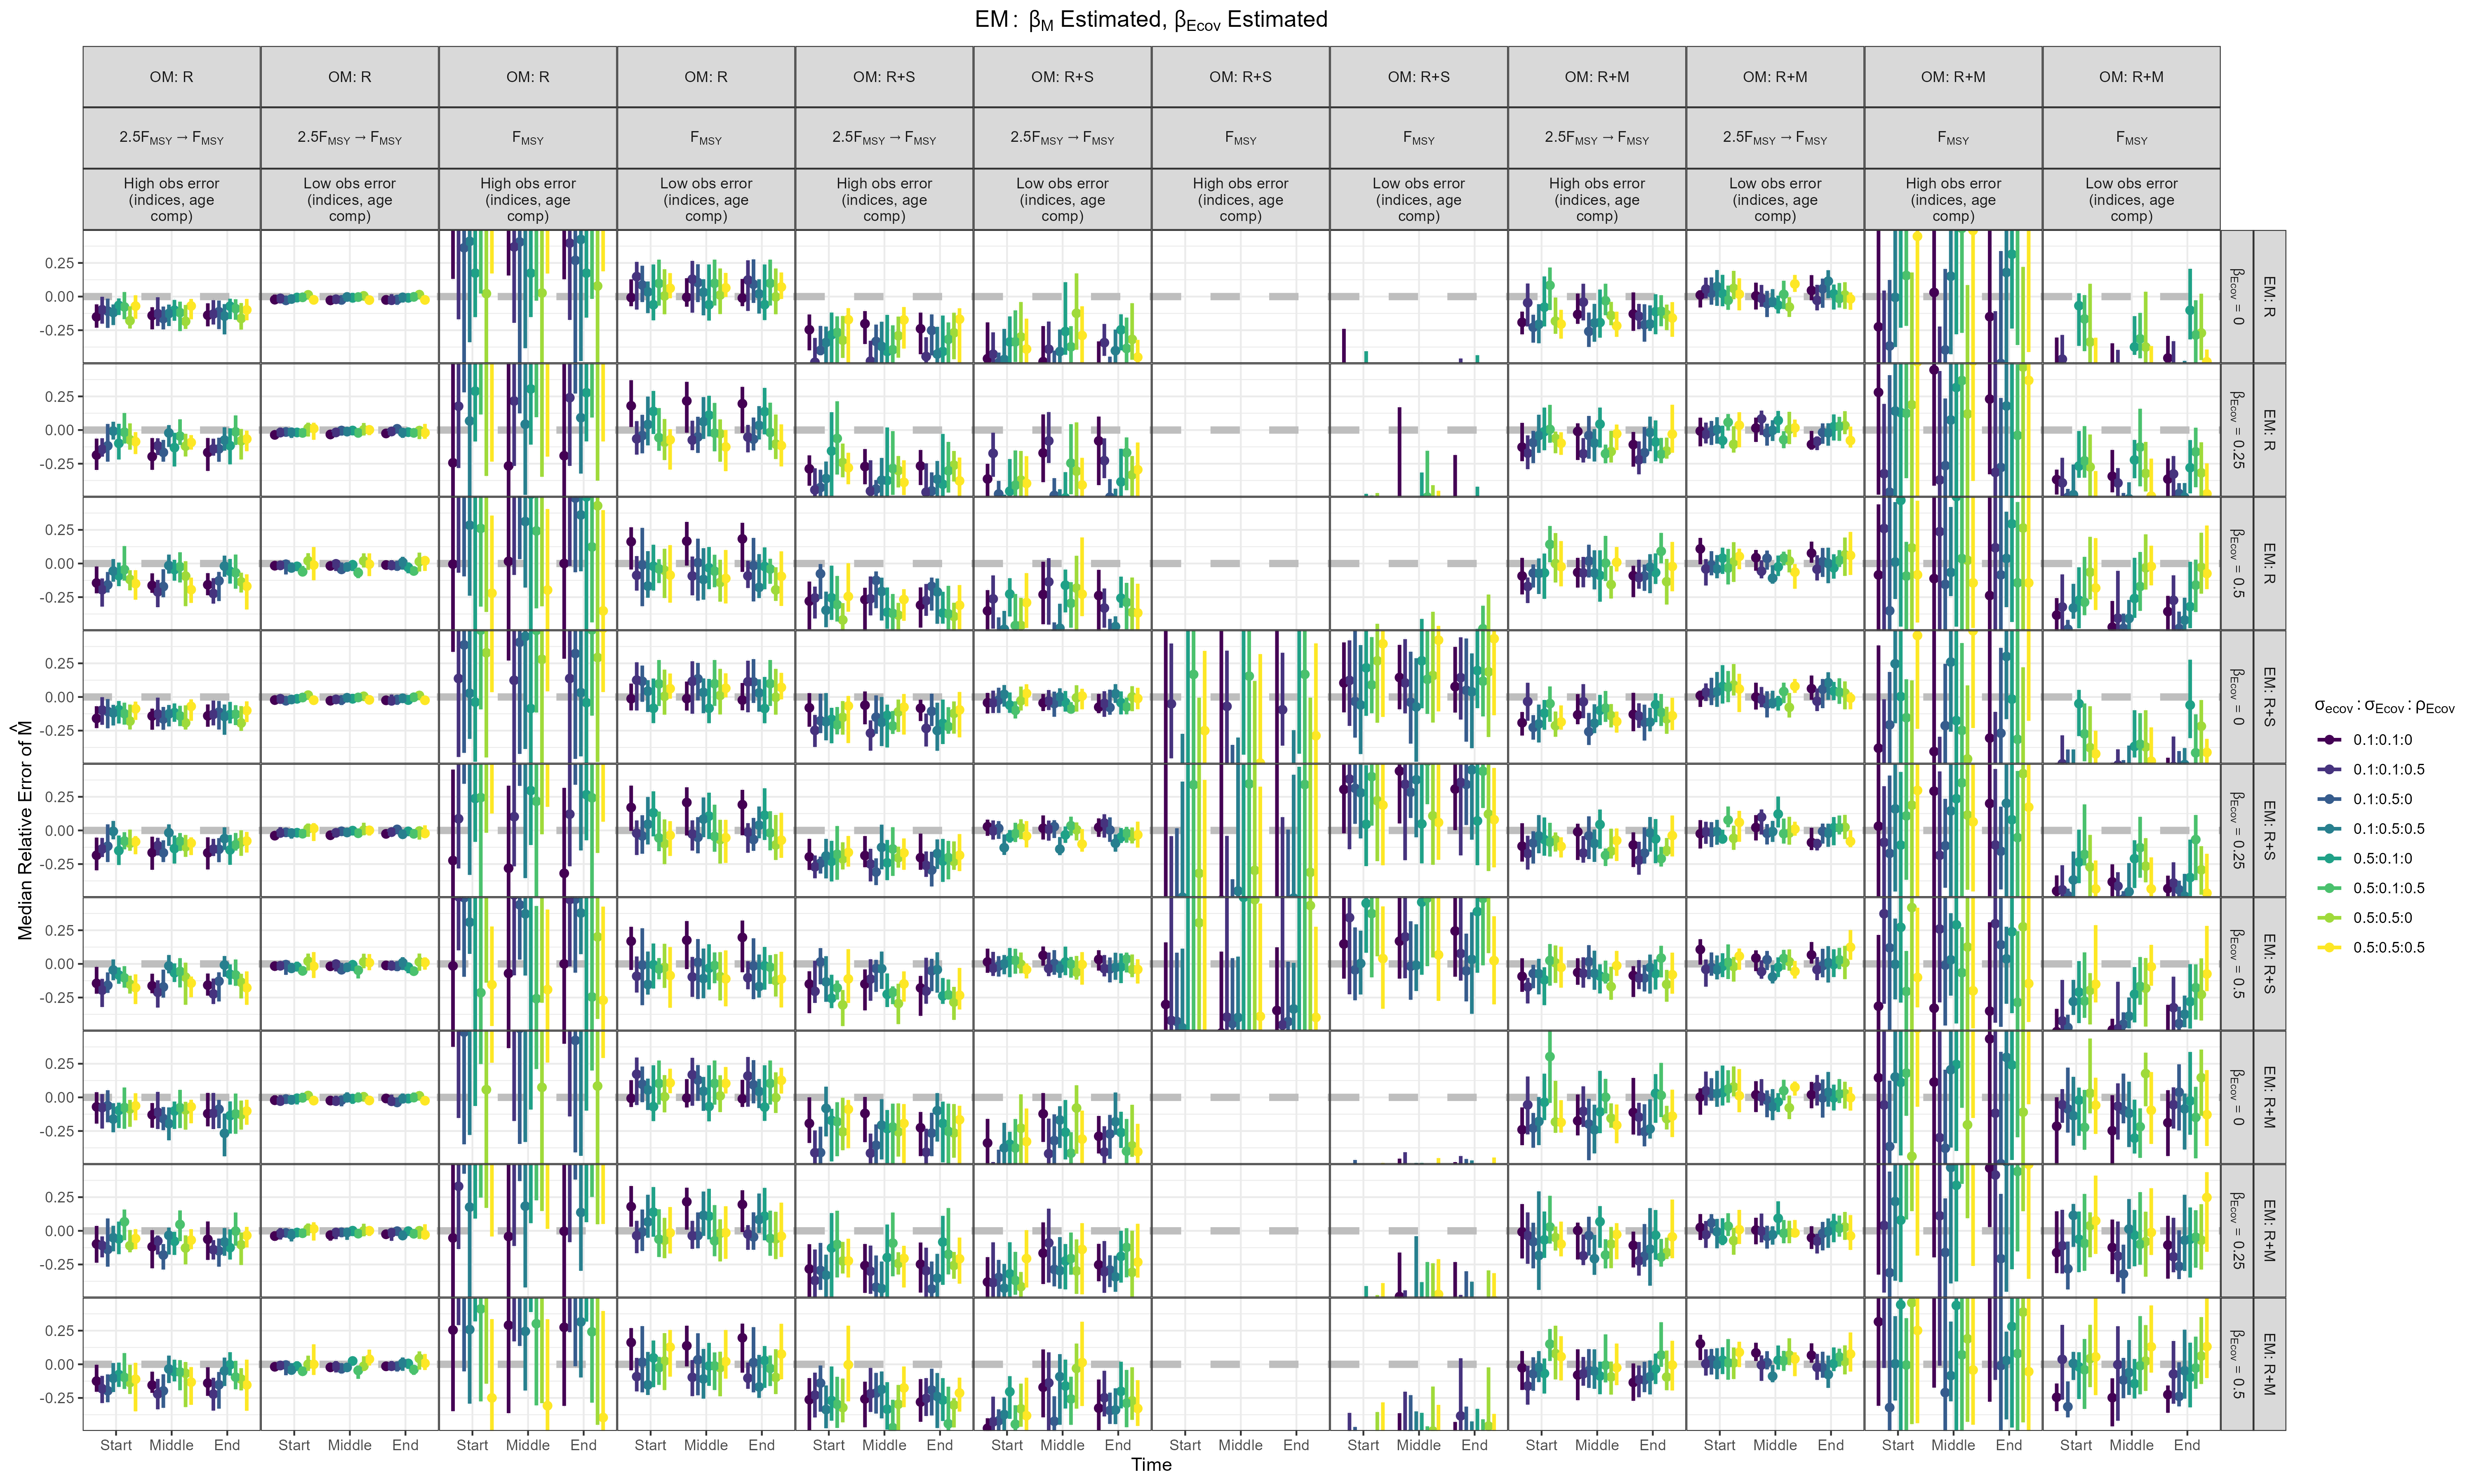
\includegraphics[height = \textheight]{annual_M_bias_all_PE_effect_M_estimated_beta_estimated.png}
\end{center}
\end{figure}
\end{landscape}

\begin{landscape}
\begin{figure}
\caption{Median relative error of annual SSB in years 1 (Start), 21 (Middle), and 40 (End) from fitting simulated observations from each operating model with alternative process error assumptions in the estimating model. Estimating models also assume the mean natural mortality parameter $\beta_\text{M} = \log 0.2$ and no environmental covariate effect $\beta_\text{Ecov} = 0$.}\label{SSB_bias_M_fixed_beta_fixed}
\begin{center}
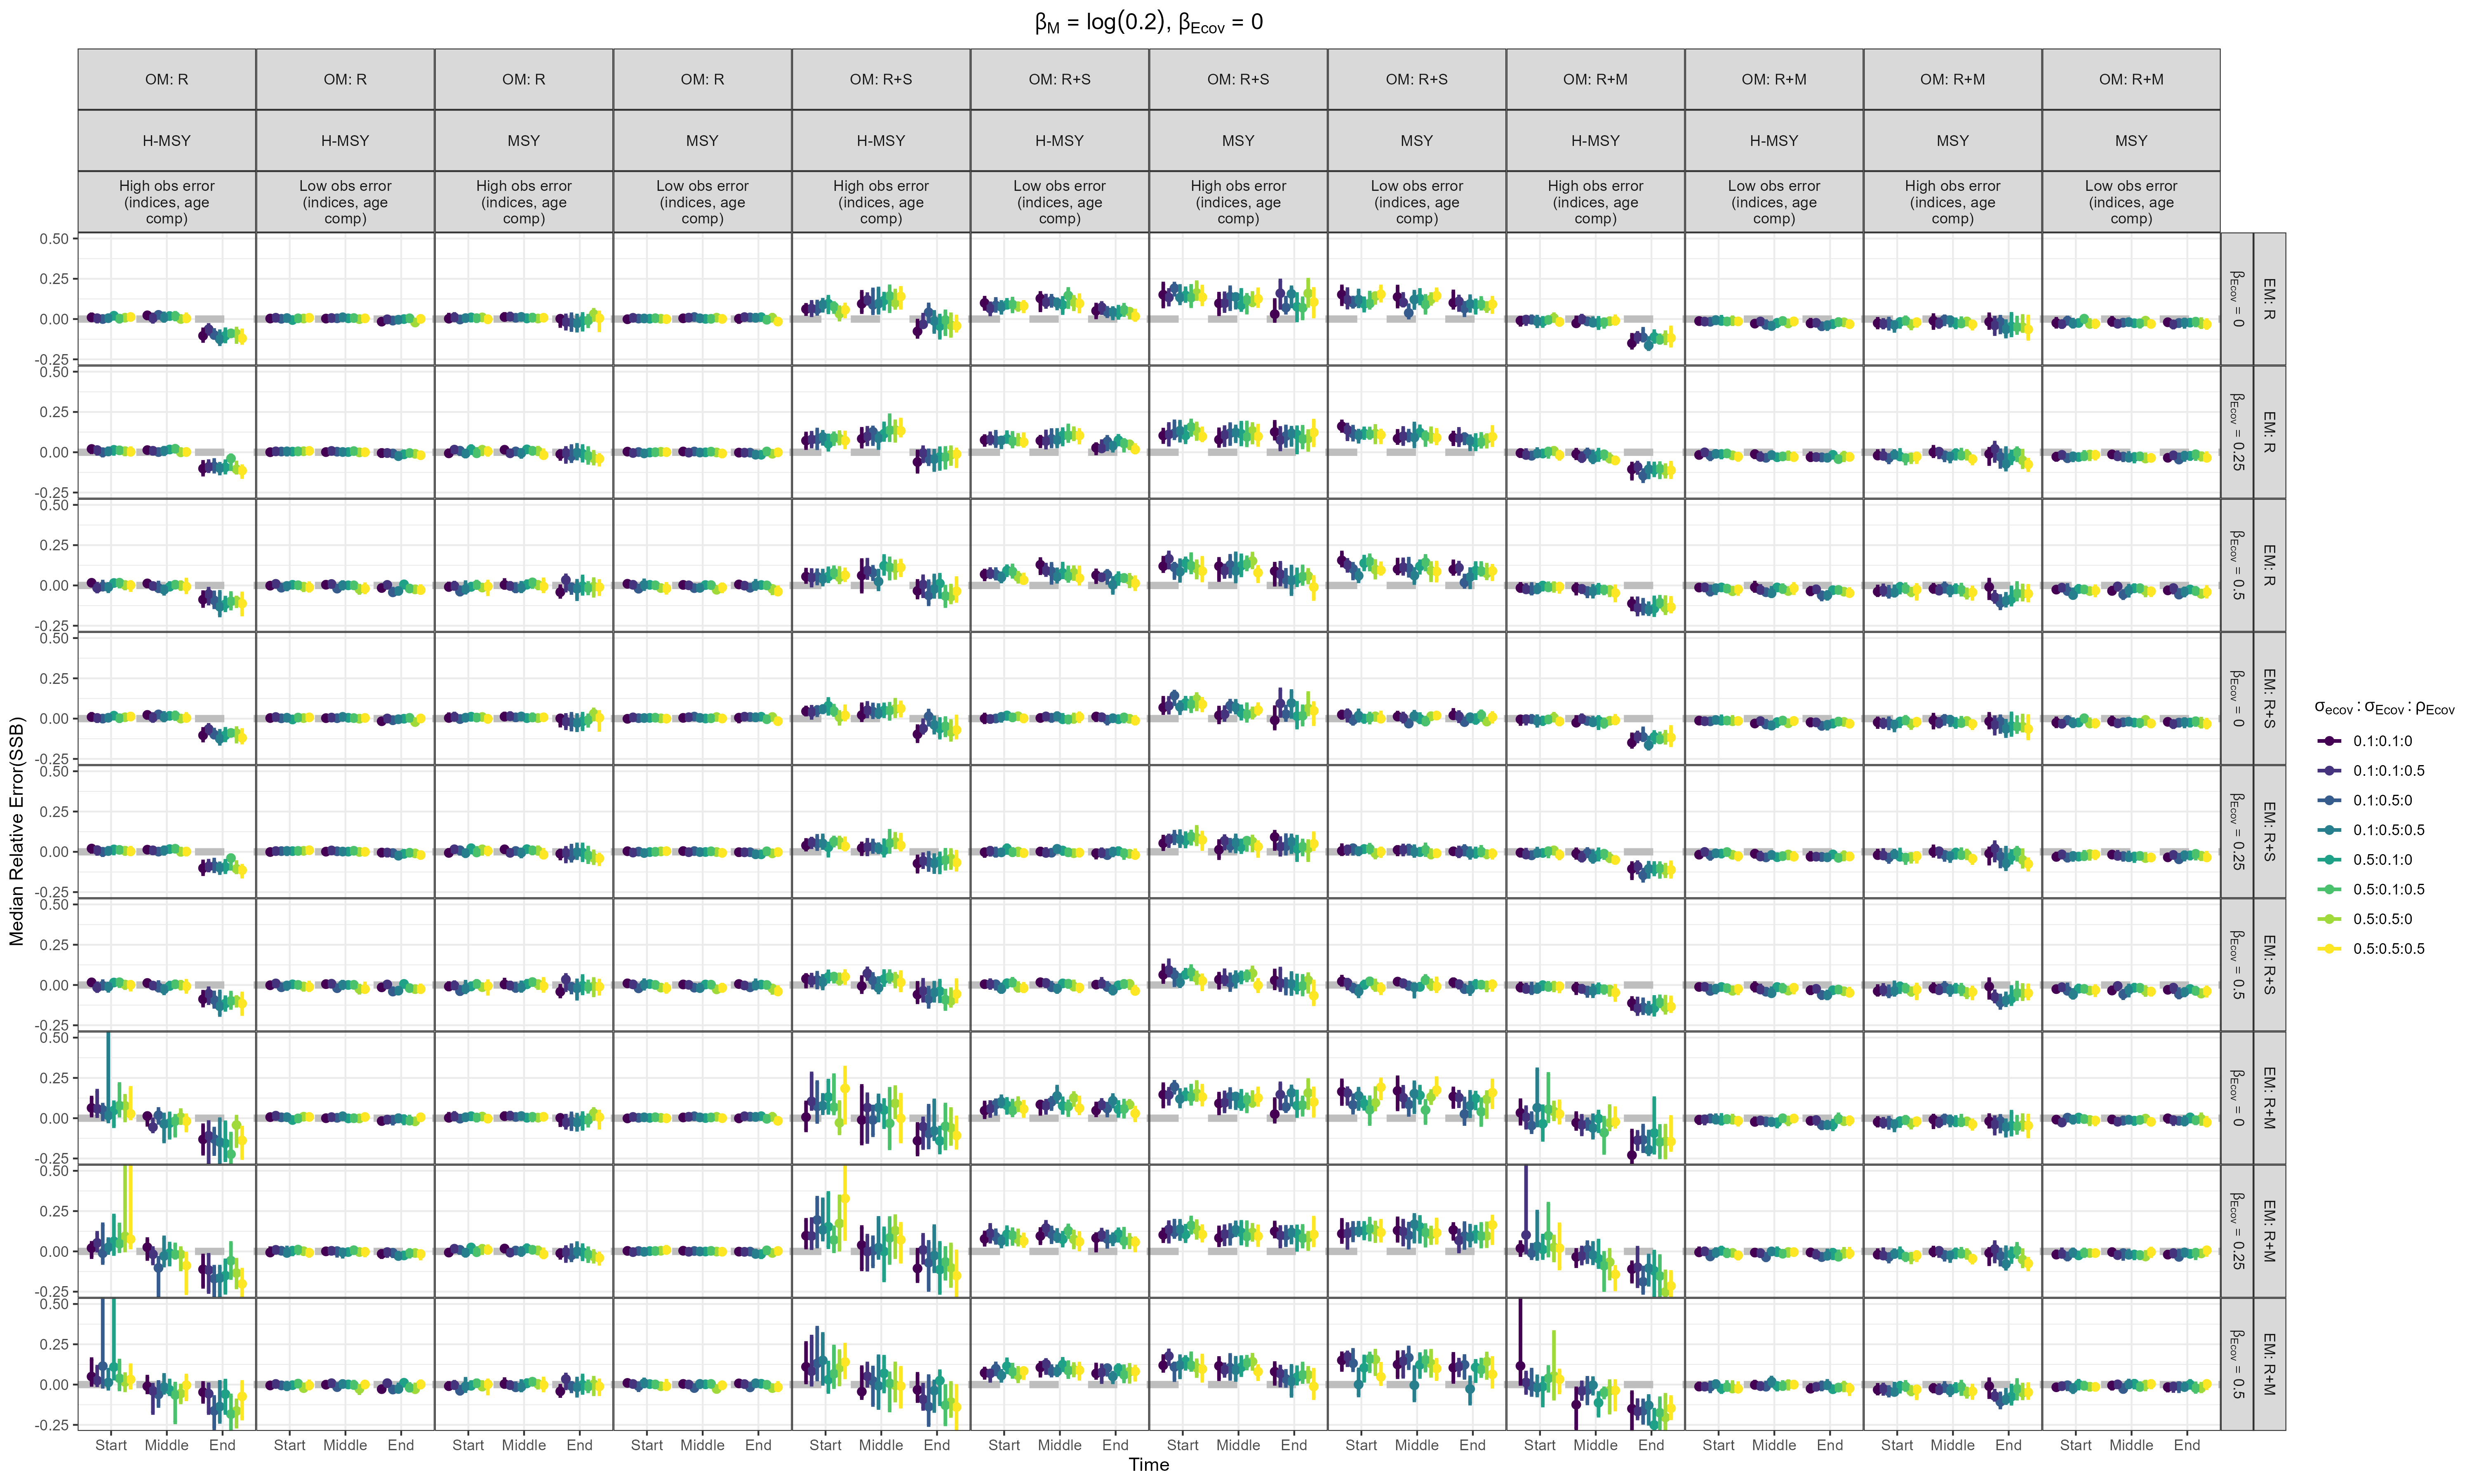
\includegraphics[height = \textheight]{SSB_bias_all_PE_effect_M_fixed_beta_fixed.png}
\end{center}
\end{figure}
\end{landscape}

\begin{landscape}
\begin{figure}
\caption{Median relative error of annual SSB in years 1 (Start), 21 (Middle), and 40 (End) from fitting simulated observations from each operating model with alternative process error assumptions in the estimating model. Estimating models also assume the mean natural mortality parameter $\beta_\text{M} = \log 0.2$ and the environmental covariate effect $\beta_\text{Ecov}$ is estimated.}\label{SSB_bias_M_fixed_beta_estimated}
\begin{center}
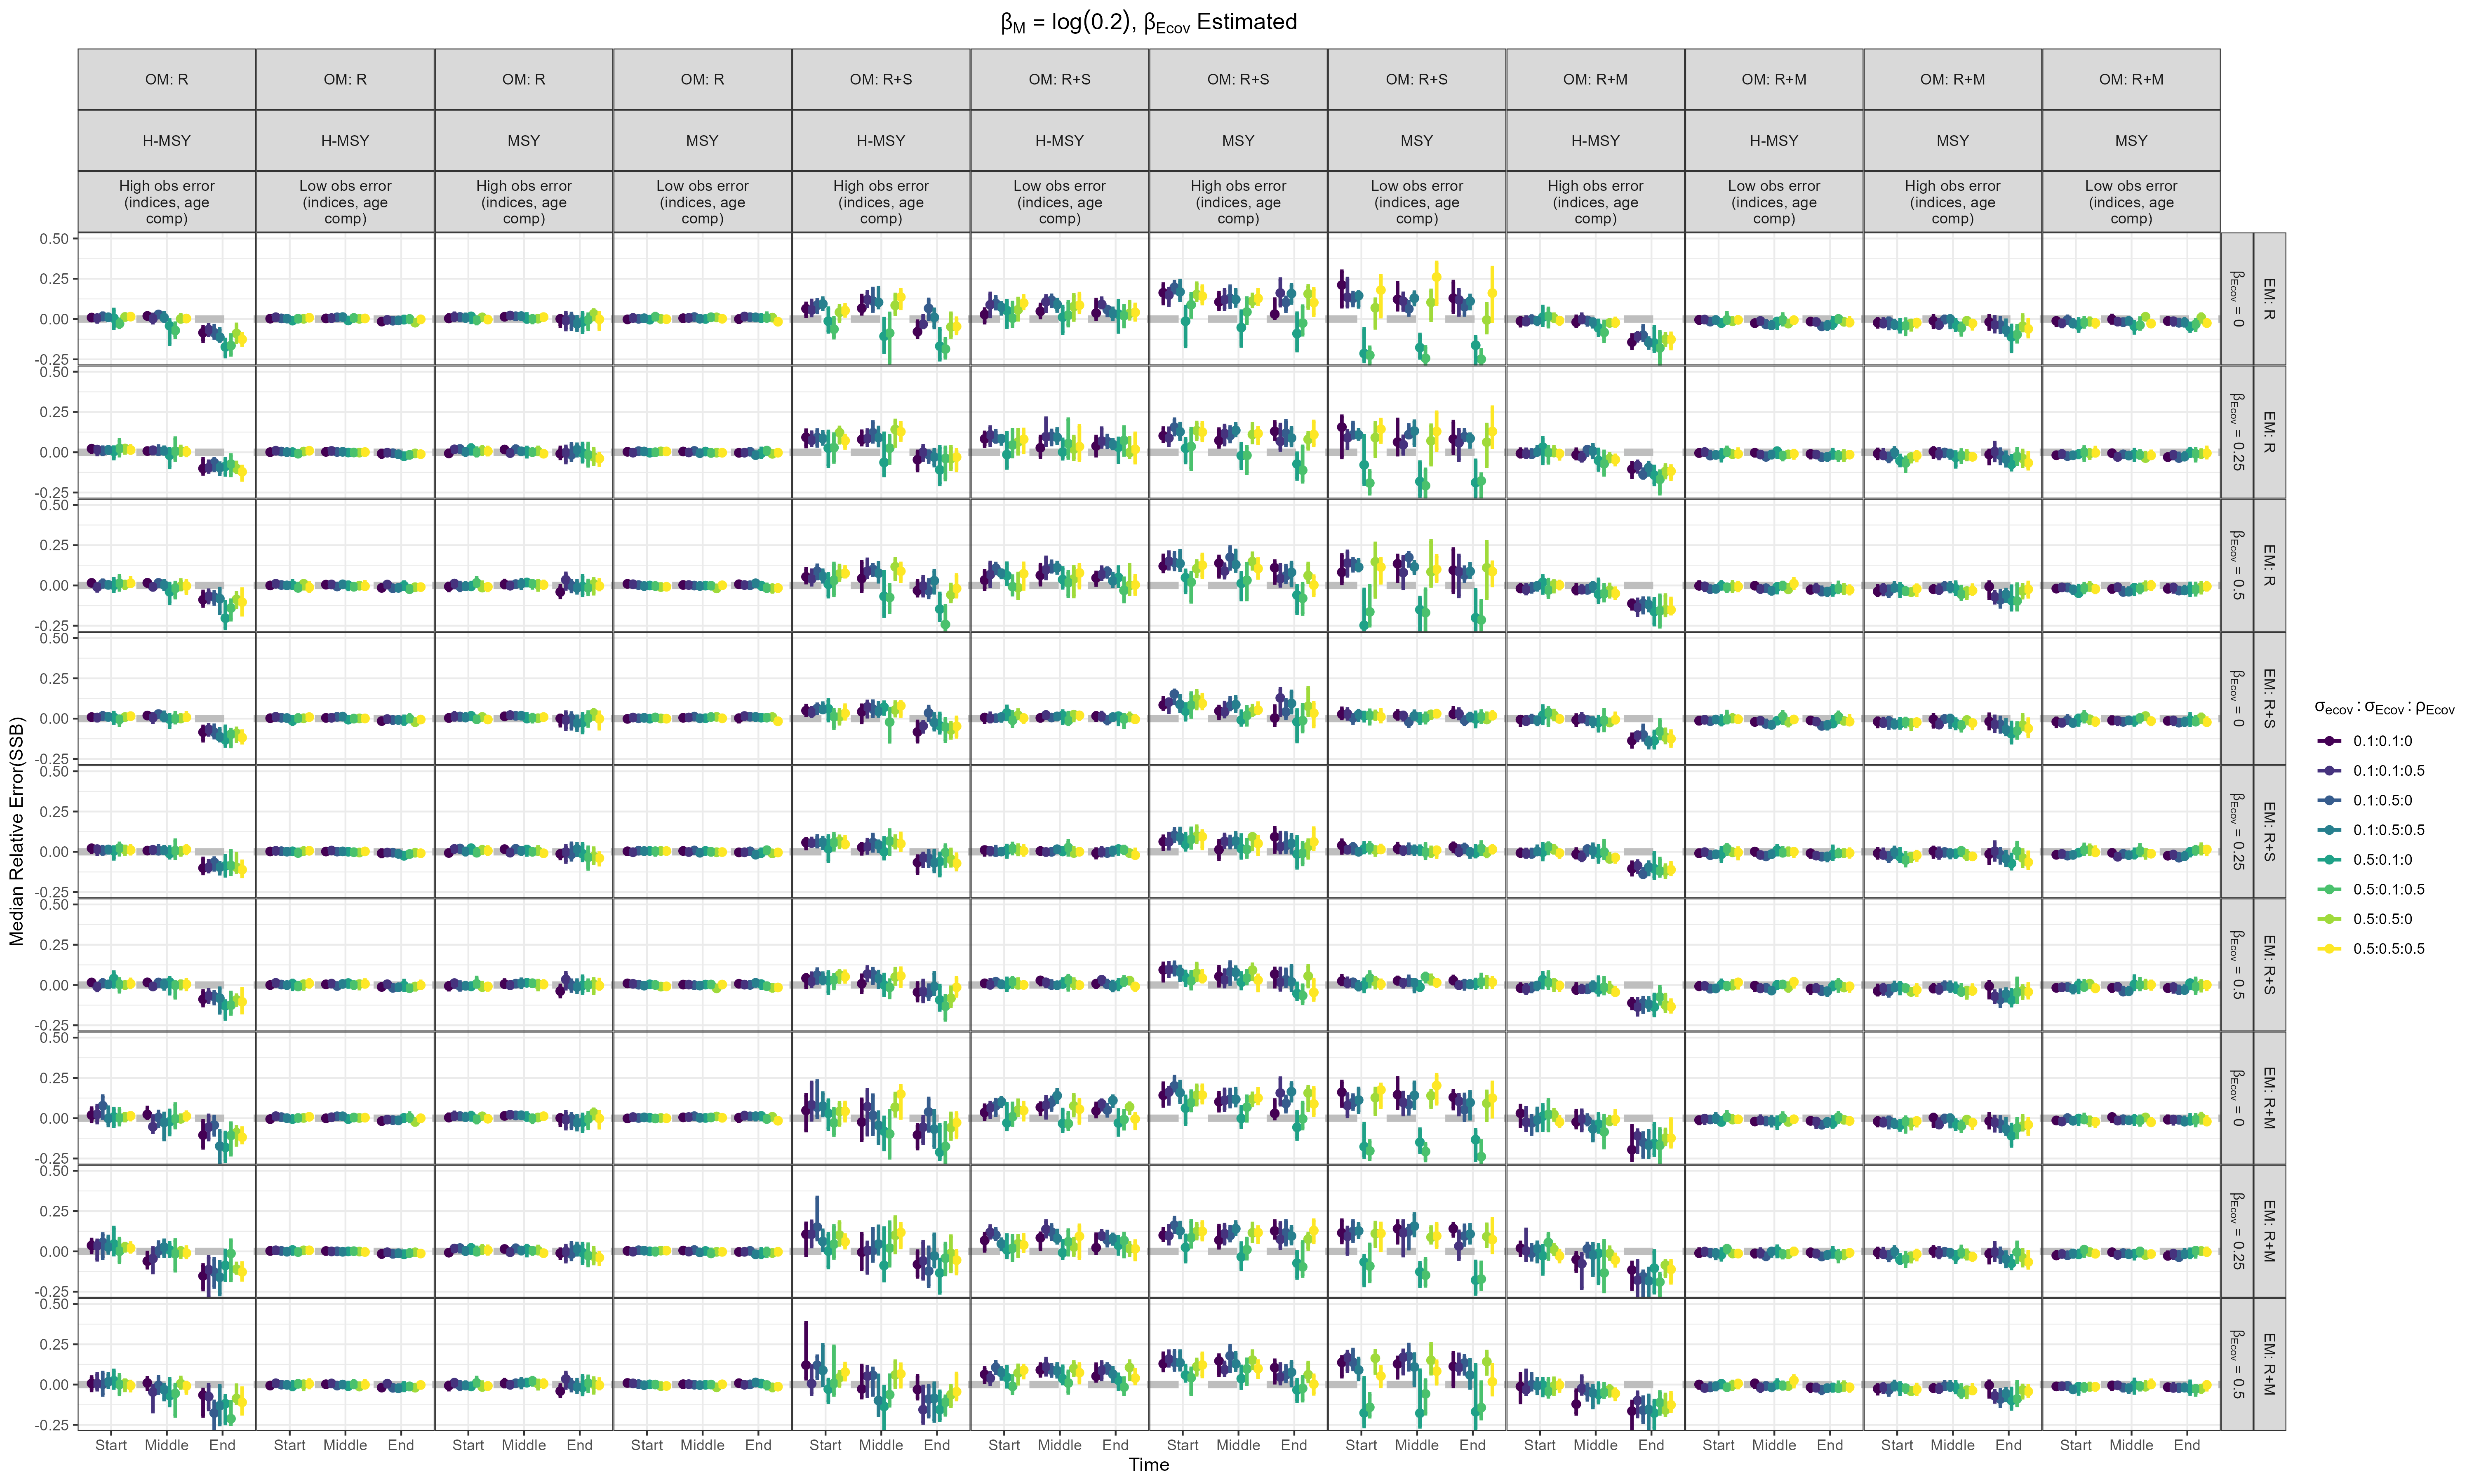
\includegraphics[height = \textheight]{SSB_bias_all_PE_effect_M_fixed_beta_estimated.png}
\end{center}
\end{figure}
\end{landscape}

\begin{landscape}
\begin{figure}
\caption{Median relative error of annual SSB in years 1 (Start), 21 (Middle), and 40 (End) from fitting simulated observations from each operating model with alternative process error assumptions in the estimating model. Estimating models also assume both the mean natural mortality parameter $\beta_\text{M}$ and the environmental covariate effect $\beta_\text{Ecov}$ are estimated.}\label{SSB_bias_M_estimated_beta_estimated}
\begin{center}
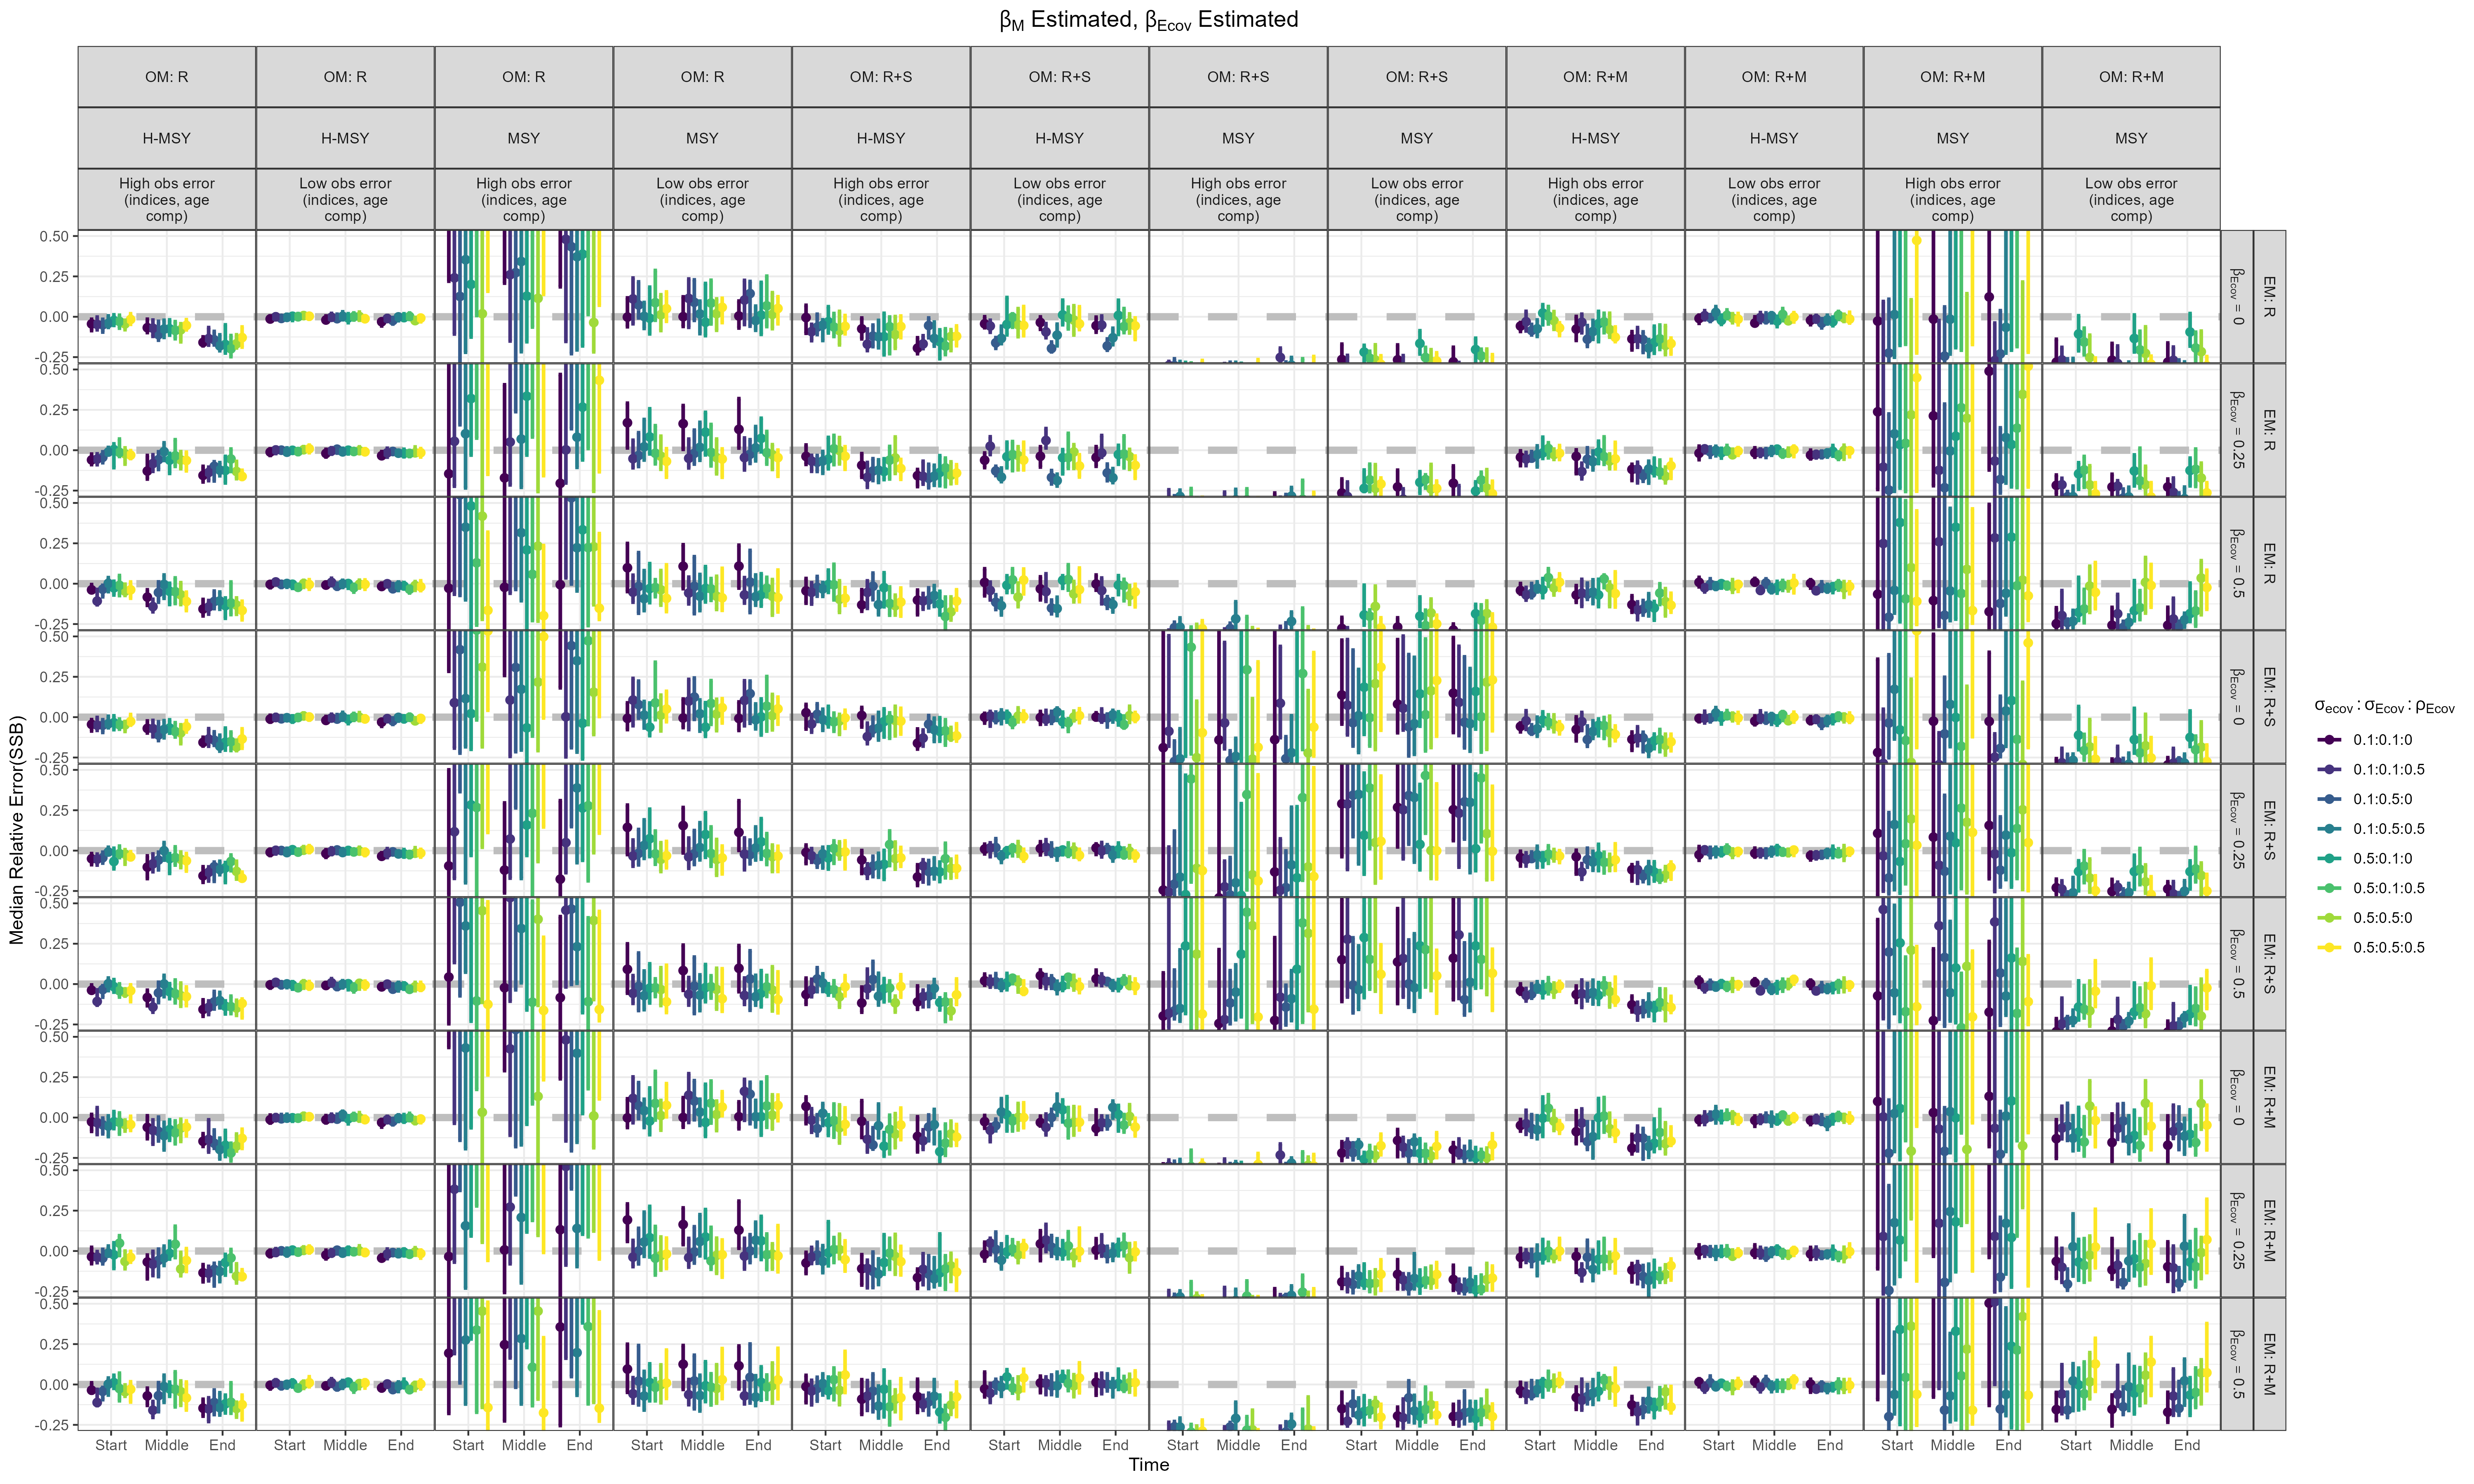
\includegraphics[height = \textheight]{SSB_bias_all_PE_effect_M_estimated_beta_estimated.png}
\end{center}
\end{figure}
\end{landscape}

\hypertarget{supplemental-materials}{%
\section*{Supplemental Materials}\label{supplemental-materials}}
\addcontentsline{toc}{section}{Supplemental Materials}

\begin{landscape}
\begin{figure}
\caption{Median relative error of annual fully-selected fishing mortality rate in years 1 (Start), 21 (Middle), and 40 (End) from fitting simulated observations from each operating model with alternative process error assumptions in the estimating model. Estimating models also assume the mean natural mortality parameter $\beta_\text{M} = \log 0.2$ and no environmental covariate effect $\beta_\text{Ecov} = 0$.}\label{F_bias_M_fixed_beta_fixed}
\begin{center}
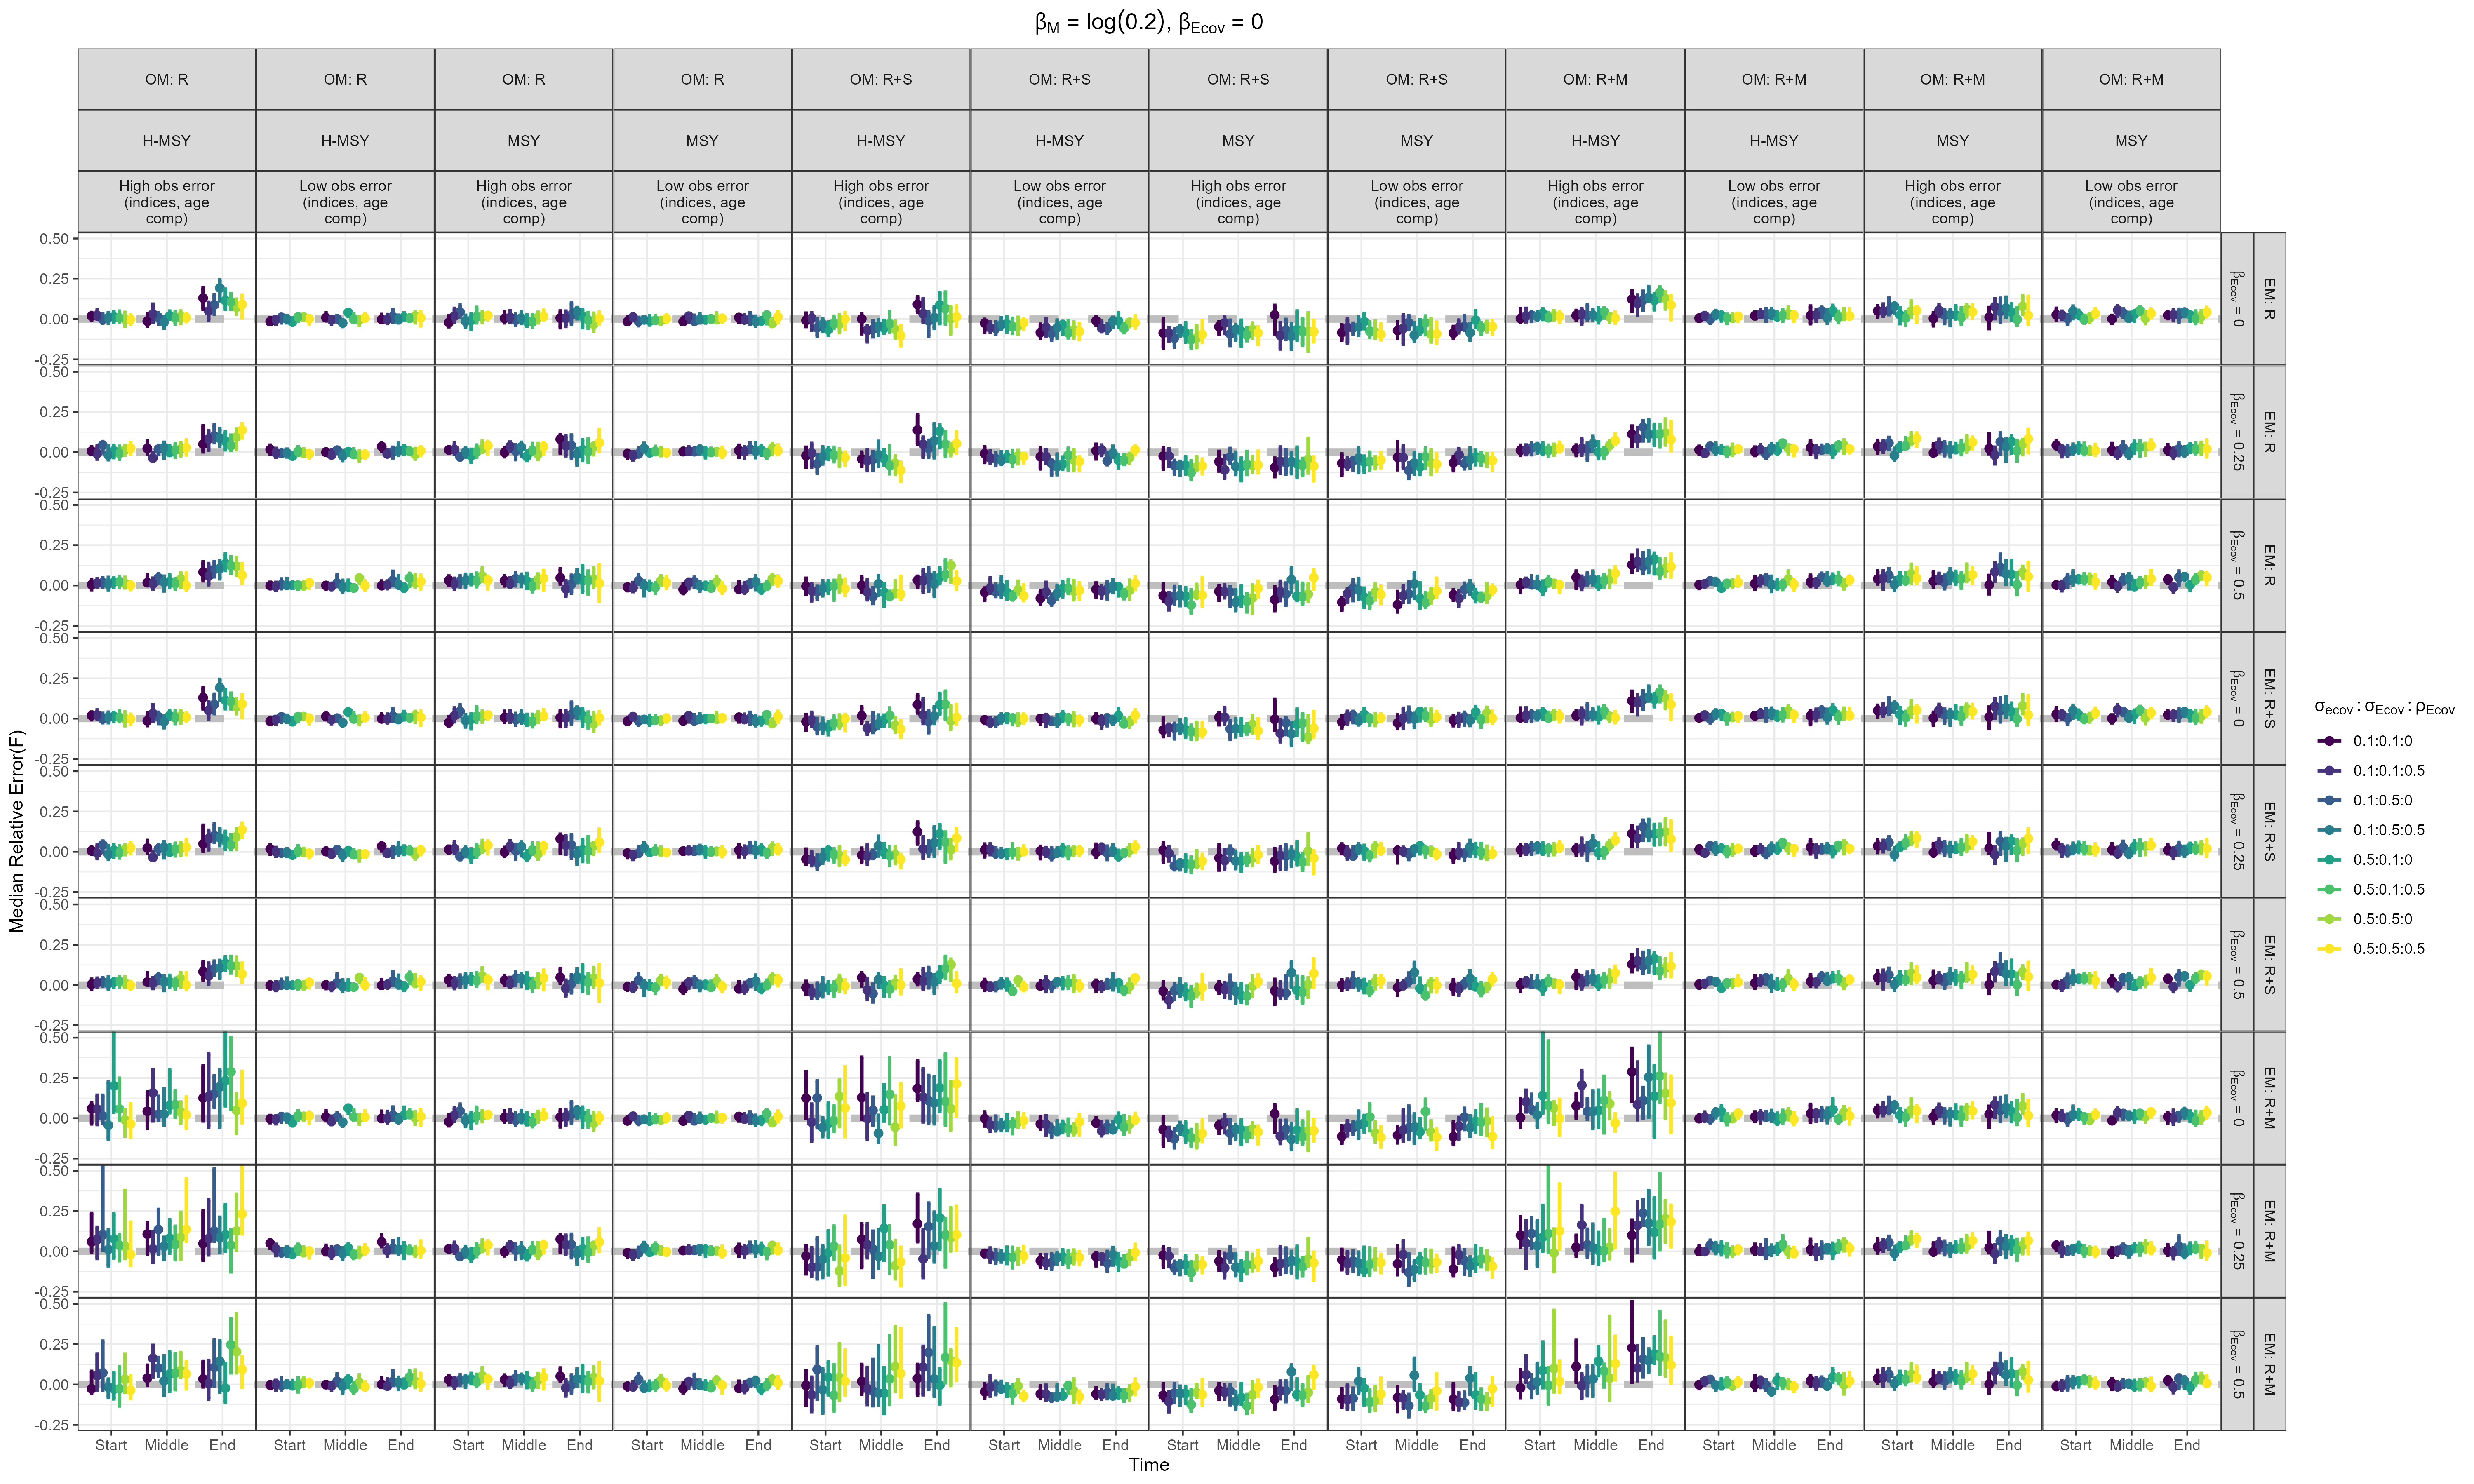
\includegraphics[height = \textheight]{F_bias_all_PE_effect_M_fixed_beta_fixed.png}
\end{center}
\end{figure}
\end{landscape}

\begin{landscape}
\begin{figure}
\caption{Median relative error of annual fully-selected fishing mortality rate in years 1 (Start), 21 (Middle), and 40 (End) from fitting simulated observations from each operating model with alternative process error assumptions in the estimating model. Estimating models also assume the mean natural mortality parameter $\beta_\text{M} = \log 0.2$ and the environmental covariate effect $\beta_\text{Ecov}$ is estimated.}\label{F_bias_M_fixed_beta_estimated}
\begin{center}
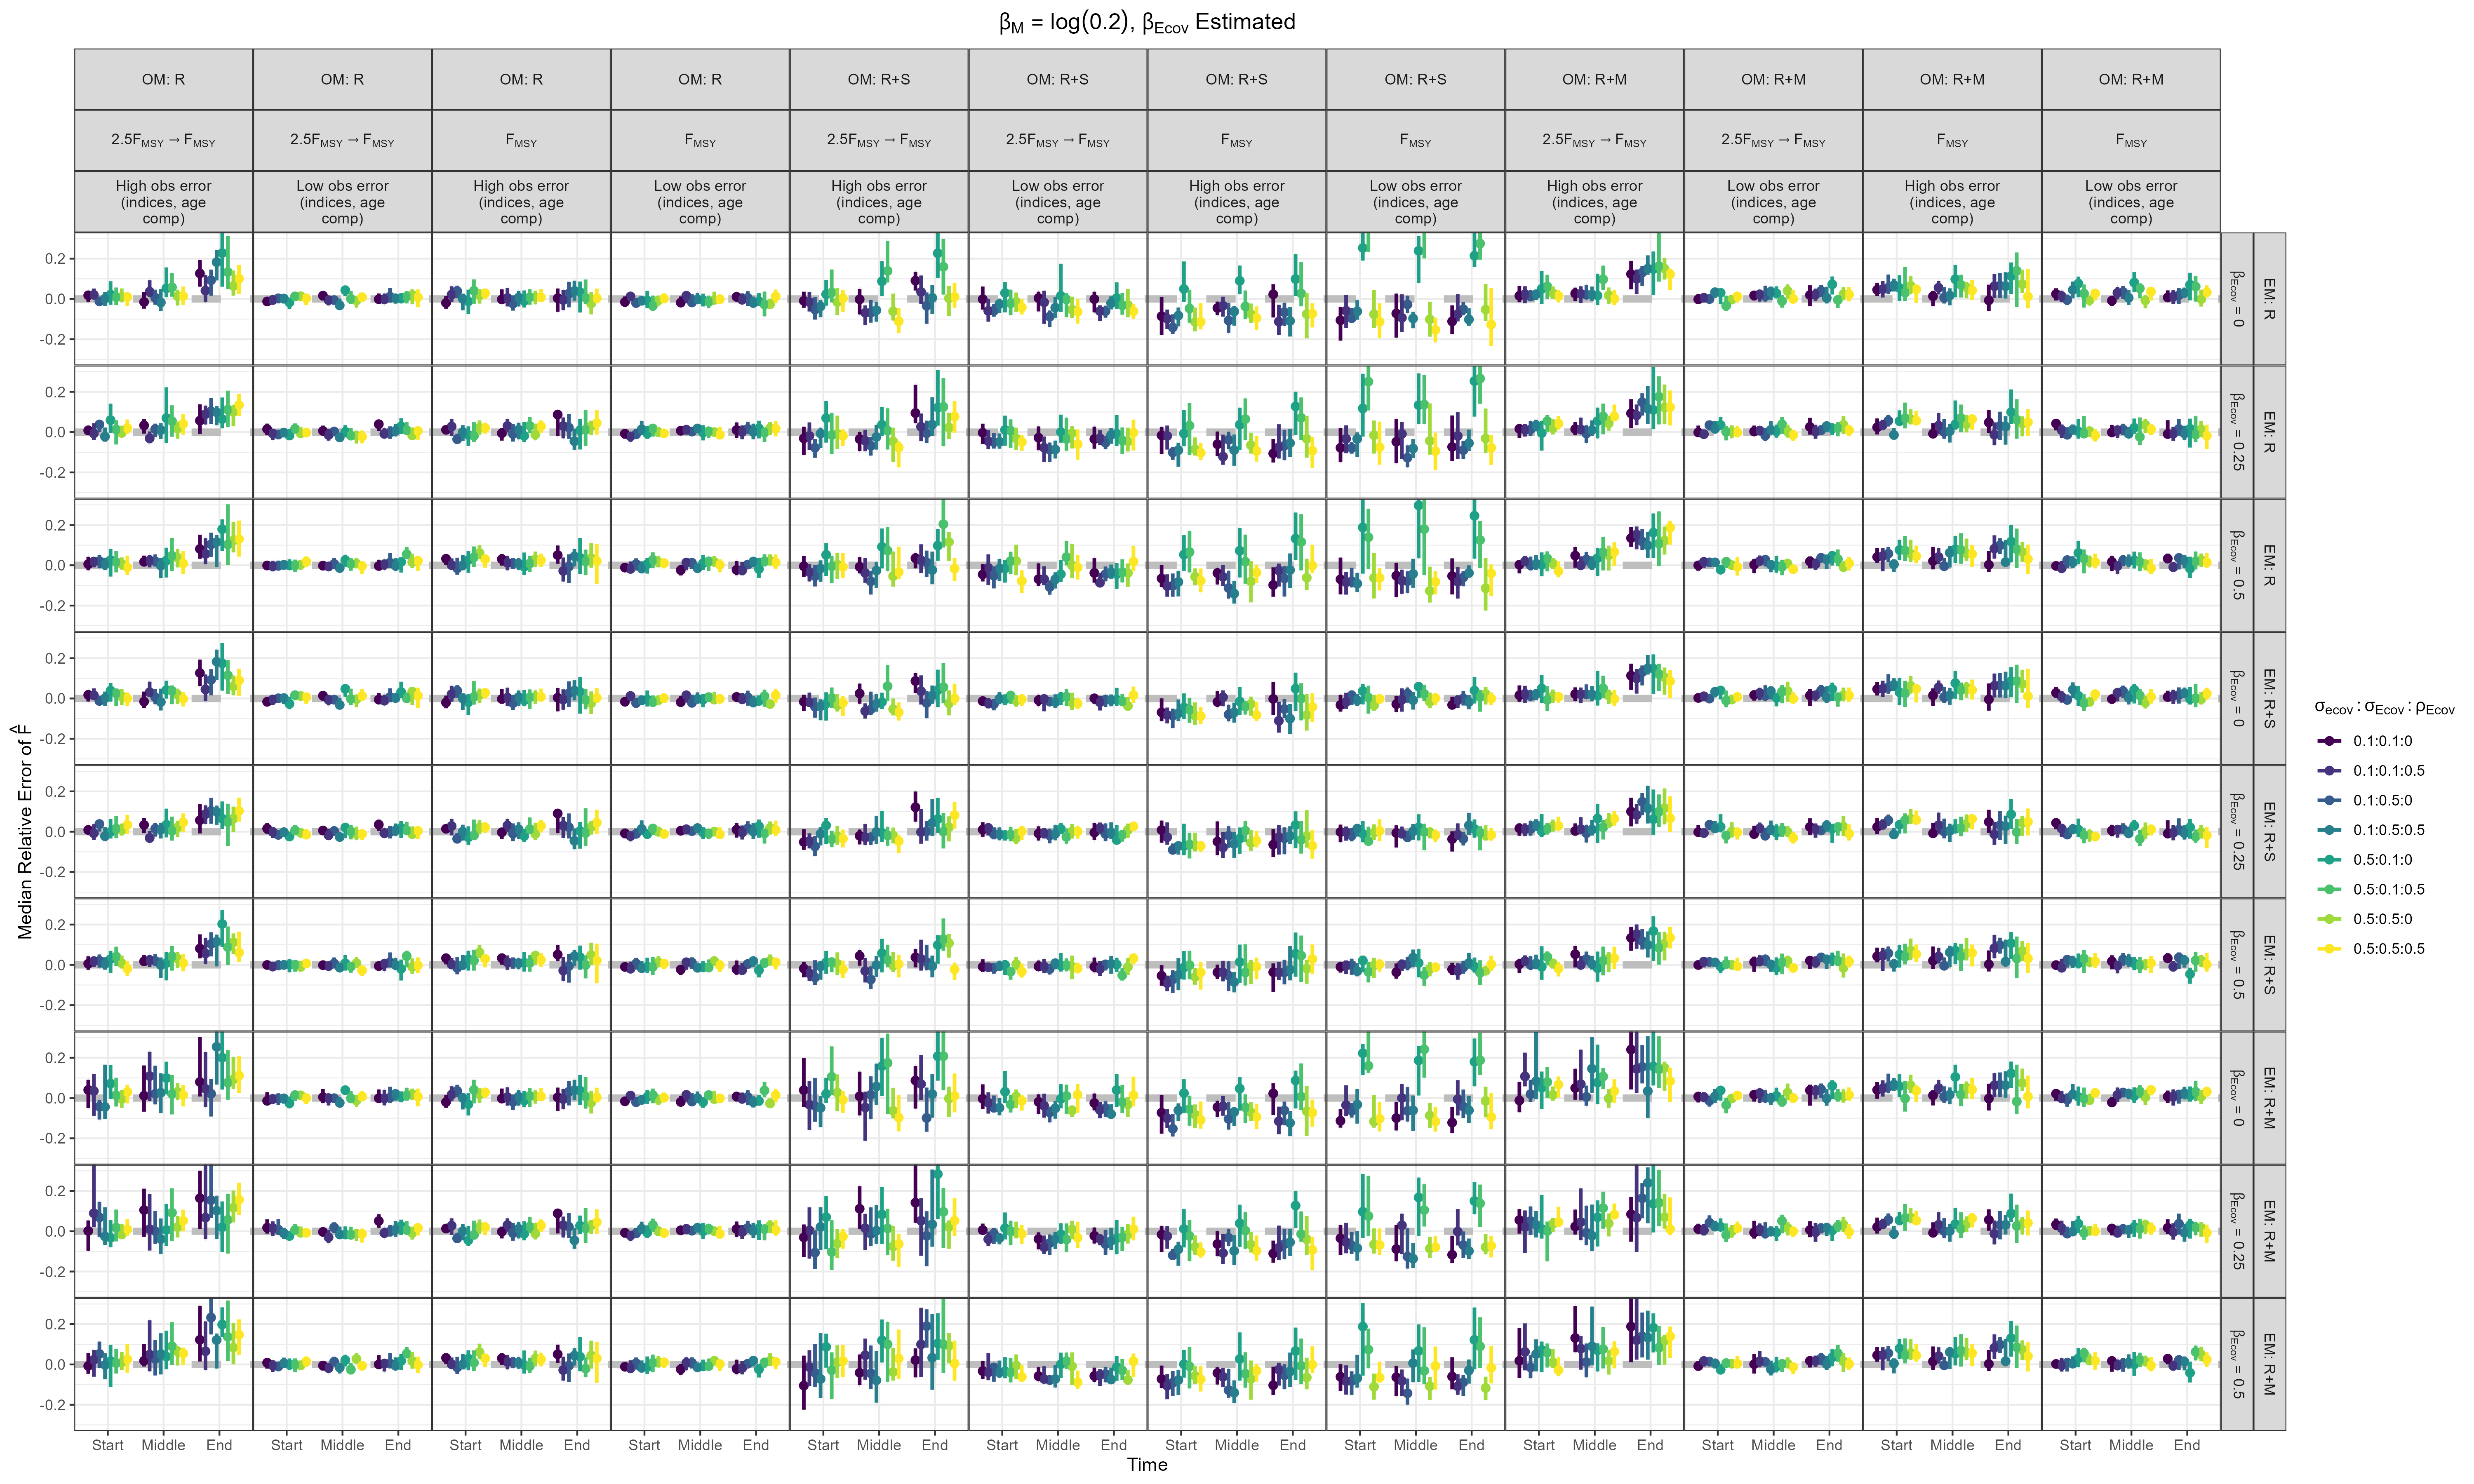
\includegraphics[height = \textheight]{F_bias_all_PE_effect_M_fixed_beta_estimated.png}
\end{center}
\end{figure}
\end{landscape}

\begin{landscape}
\begin{figure}
\caption{Median relative error of annual fully-selected fishing mortality rate in years 1 (Start), 21 (Middle), and 40 (End) from fitting simulated observations from each operating model with alternative process error assumptions in the estimating model. Estimating models also assume both the mean natural mortality parameter $\beta_\text{M}$ and the environmental covariate effect $\beta_\text{Ecov}$ are estimated.}\label{F_bias_M_estimated_beta_estimated}
\begin{center}
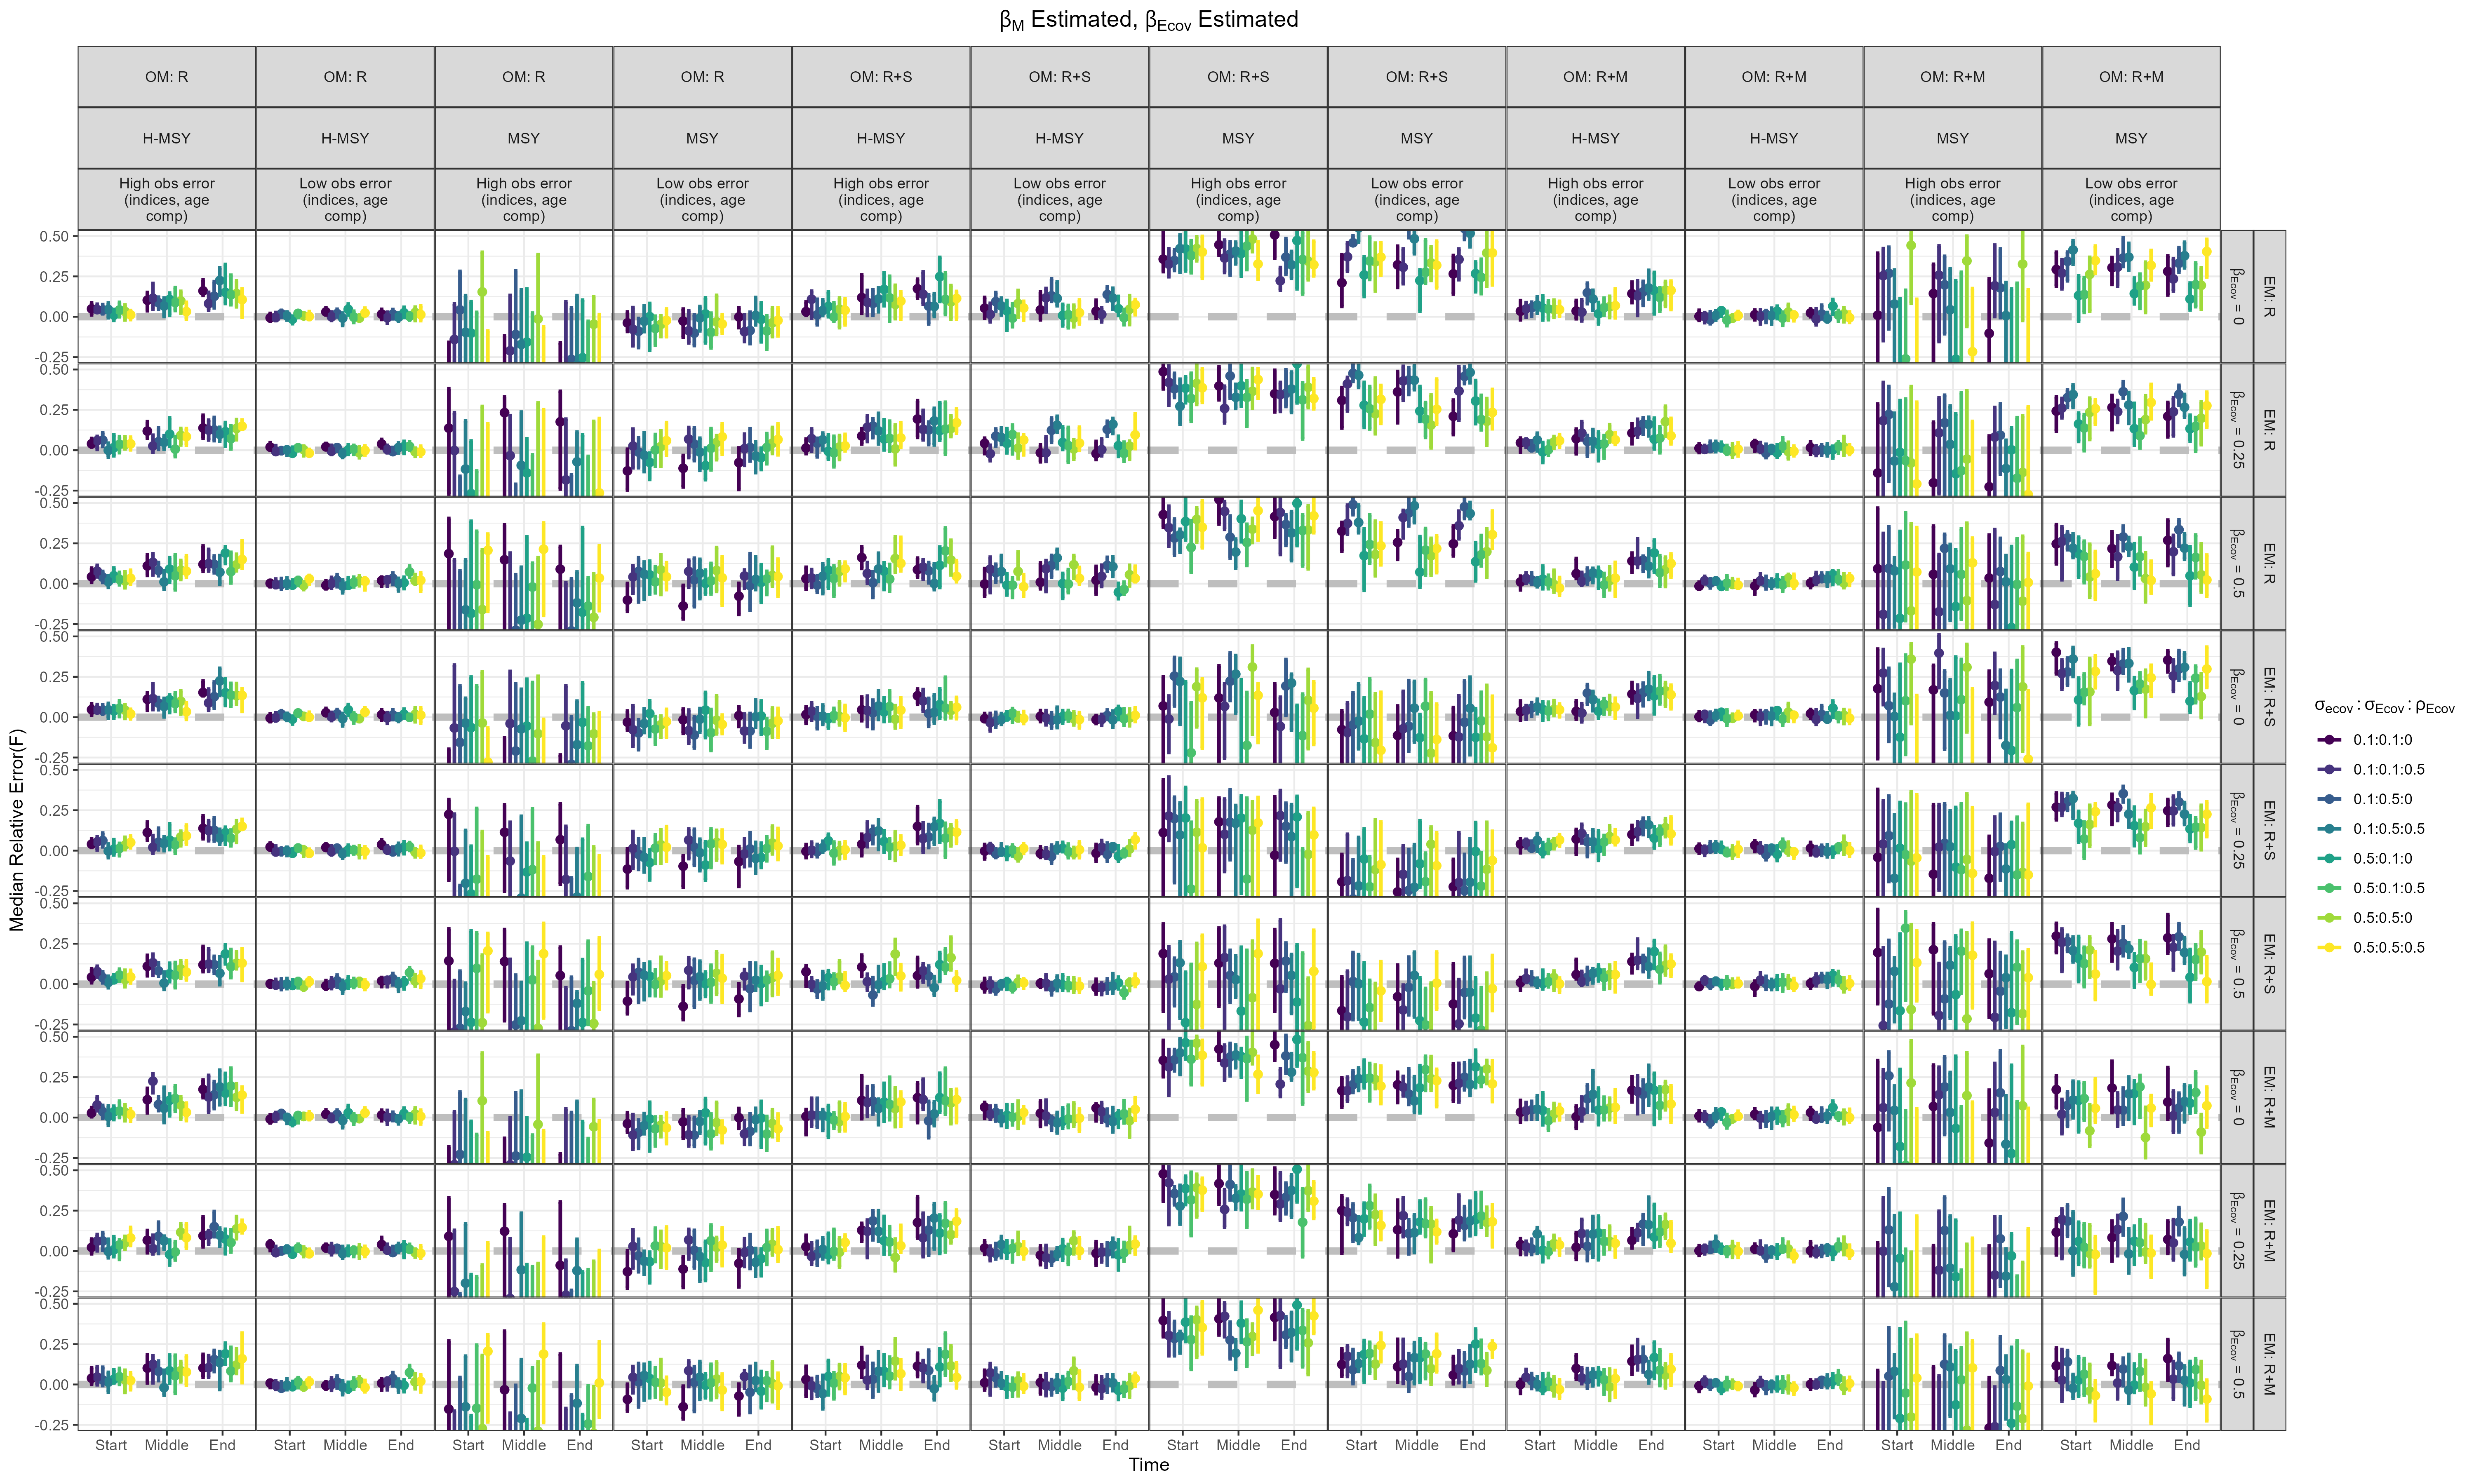
\includegraphics[height = \textheight]{F_bias_all_PE_effect_M_estimated_beta_estimated.png}
\end{center}
\end{figure}
\end{landscape}

\end{document}
